\documentclass[11pt,a4paper,headings=small,dvips]{scrbook}
\setcounter{secnumdepth}{3}
\setcounter{tocdepth}{3}
% This is used to create the cover and to plot trees
\usepackage{pst-tree}
\usepackage{pstricks,pstricks-add,multido}
%
\usepackage{geometry}
\usepackage{moresize}
%
%\usepackage{algorithmic}
% 
\usepackage{fancyvrb}
\usepackage{listings}
\usepackage{alltt}
\usepackage{gensymb}
%
\usepackage[section]{placeins}
% 
\usepackage{pbox}
% http://en.wikibooks.org/wiki/LaTeX/Indexing
\usepackage{makeidx} 
\makeindex
%
%\usepackage{subfigure}
% Figure caption settings
\usepackage[textfont=it,margin=10pt,font=small,labelfont=bf,labelsep=endash]{caption}
\usepackage{subcaption}
%
\usepackage{bm}
% Landscape package
\usepackage{lscape}
%
\usepackage{hyperref} 
\hypersetup{colorlinks=true}
\hypersetup{breaklinks=true}
% package for multiline comments
\usepackage{verbatim}
%
% Package to create a glossary - It must be uploaded after hyperref
% to produce the glossary: makeglossaries OQB
%\usepackage[toc,acronym,nonumberlist,style=altlist]{glossaries}
\usepackage[toc,nonumberlist,style=altlist]{glossaries}
\glstoctrue
\makeglossaries
%
% - - - - - - - - - - - - - - - - - - - - - - - - - - - - - - - - Setting Fonts
% \renewcommand{\encodingdefault}{OT1}
\renewcommand{\encodingdefault}{OT1}
\renewcommand{\familydefault}{ppl}
% \renewcommand{\familydefault}{cmss}
% \renewcommand{\seriesdefault}{m}
% \renewcommand{\shapedefault}{up}

% - - - - - - - - - - - - - - - - - - - - - - - - - - - - - - - - - - - - - - -
\usepackage{amsmath}
% - - - - - - - - - - - - - - - - - - - - - - - - - - - - - - - - - - - - - - -
\usepackage{titlesec}
\usepackage[dvips]{graphicx}
% - - - - - - - - - - - - - - - - - - - - - - - - - - - - - - - - - - - - - - -
\usepackage{type1cm,eso-pic,color}

%\makeatletter
%\AddToShipoutPicture{
%    \setlength{\@tempdimb}{.5\paperwidth}
%    \setlength{\@tempdimc}{.5\paperheight}
%    \setlength{\unitlength}{1pt}
%    \put(\strip@pt\@tempdimb,\strip@pt\@tempdimc){
%        \makebox(0,0){\rotatebox{55}{
%        	\textcolor[gray]{0.85}{
%        		\fontsize{5cm}{5cm}
%        		\selectfont{DRAFT}}
%        	}
%        }
%	}
%}
%\makeatother

%
% Solves problems with margin notes
\usepackage{mparhack} 
	\setlength{\marginparwidth}{1.1in}
	\let\oldmarginpar\marginpar
	\renewcommand\marginpar[1]{\-\oldmarginpar[\raggedright\color{red01}
	\footnotesize #1]%
	{\raggedright\footnotesize #1}}
% Define some colors
	\definecolor{azure}{RGB}{240,255,255}
	\definecolor{honeydew}{RGB}{240,255,240}
	\definecolor{blue01}{RGB}{4,64,116}
	\definecolor{blue02}{RGB}{0,62,113}
	\definecolor{gray01}{rgb}{0.1,0.1,0.1}
	\definecolor{gray02}{rgb}{0.8,0.8,0.8}
	\definecolor{red01}{rgb}{0.5,0.0,0.0}
	\definecolor{orange00}{rgb}{1.0,0.74,0.53}
	\definecolor{orange01}{rgb}{0.9137,0.5882,0.0980}
	\definecolor{orange02}{rgb}{0.7608,0.4157,0.1804}
	\definecolor{orange03}{rgb}{0.6941,0.1843,0.1333}
\usepackage[english]{babel}
% Bibliography settings
\usepackage[square,colon]{natbib} % Extend bibligraphy functions
% Page numbering by Chapter
%\usepackage[auto]{chappg} 
%\pagenumbering{bychapter}
% 
% Define page properties
\usepackage{scrpage2}
	\pagestyle{scrheadings}
	\lofoot[]{
\includegraphics[width=2.0cm]{./figures/openquake_logo1.eps}}
	\refoot[]{
\includegraphics[width=2.0cm]{./figures/openquake_logo1.eps}}
	%\renewcommand{\partpagestyle}{empty}
% - - - - - - - - - - - - - - - - - - - - - - - - - -  Reformatting PART Titles
\titleformat{\part}[display]
{\filleft\normalfont\sffamily}
{\textcolor{blue01}{\bfseries\large PART}\hspace{4pt}
	\bfseries\Huge\textcolor{blue01}{\thepart}}
{1pc}
{\Huge\bfseries\textcolor{blue01}}
[]
% - - - - - - - - - - - - - - - - - - - - - - - - - Reformatting CHAPTER Titles
% Titles: CHAPTER
\titleformat{\chapter}
	[display] % shape
	{\filleft\normalfont\sffamily} % format
	{\textcolor{blue01}{\bfseries\MakeUppercase{\chaptertitlename}} % label
	\hspace{4pt}\huge\bfseries\textcolor{blue01}{\thechapter}} 
	{1pc} % sep
	{\huge\bfseries\textcolor{blue01}} % Before
	[]
% - - - - - - - - - - - - - - - - - - - - - - - - - Reformatting SECTION Titles
% Titles: SECTION
\titleformat{\section}
	[hang] % shape
	{\vspace{.8ex}\Large\bfseries\color{blue01}} % format 
	{\textcolor{blue01}{\thesection.}} % label
	{.5em} % sep
	{} % before
	[] % after
% - - - - - - - - - - - - - - - - - - - - - - -  Reformatting SUBSECTION Titles
% Title: SUBSECTION
\titleformat{\subsection}
	[hang] % shape
	{\vspace{.8ex}\large\bfseries\color{blue01}} % format 
	{\textcolor{blue01}{\thesubsection.}} % label
	{.5em} % sep
	{} % before
	[] % after
%  - - - - - - - - - - - - - - - - - - - - -  Reformatting SUBSUBSECTION Titles 
% Title: SUBSUBSECTION
\titleformat{\subsubsection}
	[hang] % shape
	{\vspace{.8ex}\normalfont\bfseries\color{blue01}} % format 
	{\textcolor{blue01}{\thesubsubsection.}} % label
	{.5em} % sep
	{} % before
	[] % after
% - - - - - - - - - - - - - - - - - - - - - - -  Reformatting PARAGRAPH Titles 
% Title: PARAGRAPH
\titleformat{\paragraph}
	[hang] % shape
	{\vspace{.2ex}\normalfont\color{blue01}} % format 
	{} % label
	{} % sep
	{} % before
	[] % after
%

\usepackage{xcolor}
\usepackage{framed}
\usepackage[utf8]{inputenc}
\usepackage{listings}

\newenvironment{myfancybox}{%
  \def\FrameCommand{\fboxsep=\FrameSep \fcolorbox{blue01}{honeydew}}%
  \color{black}\MakeFramed {\FrameRestore}}%
 {\endMakeFramed}

\setlength{\parskip}{2.5mm}
\setlength{\parindent}{0.0mm}

\begin{document}
\setcounter{page}{1}
\lstset{language=Python}

\begin{titlepage}
	\title{ \textcolor{blue01}{\textsf{\bfseries\Huge 
        Hazard Modeller's Toolkit
        }}}
	\subtitle{ \textcolor{blue01}{\textsf{\bfseries\LARGE
        Documentation \& Tutorial}}}
	\date{June 2014}
 
	\publishers{GEM Foundation, Pavia}
\end{titlepage}
\pagestyle{scrheadings}
\maketitle
% - - - - - - - - - - - - - - - - - - - - - - - - - - - - - -  Load the glossary
%\input{glossary.tex}
% -----------------------------------------------------------------------------
% -----------------------------------------------------------------------------
%\chapter*{Introduction}
%\cleardoublepage
% -----------------------------------------------------------------------------
% -----------------------------------------------------------------------------
\tableofcontents
\cleardoublepage
% 
% % -----------------------------------------------------------------------------
\chapter{Introduction to the Hazard Modeller's Toolkit}
\begin{myfancybox}
The objectives of this chapter are:
\begin{itemize}
    \item Outline the purpose and creation of the Hazard Modeller's Toolkit 
    \item Setup and installation of the software
    \item Introduction to the visualisation and mapping functions
\end{itemize}
\end{myfancybox}
  The Hazard Modeller's Toolkit (or ''hmtk'') is a Python 2.7 library of functions written by scientists at the GEM Model Facility, which is intended to provide 
scientists and engineers with the tools to help create the seismogenic 
input models that go into the OpenQuake hazard engine. The process of 
developing building the hazard model is a complex and often challenging 
one, and whilst many aspect of the practice are relatively common, the 
choice of certain methods or tools for undertaking each step can be a 
matter of judgement. The intention of this software is to provide 
scientists and engineers with the means to apply many of the most 
commonly used algorithms for preparing seismogenic source models 
using seismicity and geological data. It is still in an early 
stage of development and the current versions contain only a preliminary
set of tools for undertaking the necessary workflows. In forthcoming 
versions will hope to make available more tools for the current processes
indicated here, and to integrate new functionalities for i) merging and
homogenisation of earthquake catalogues, ii) calculation of activity 
rates from geological and geodetic data, iii) testing and interpretation
of Ground Motion Prediction Equations, and iv) integration of 
seismological and geological data and treatment of uncertainty 
in the construction of seismogenic source zones.

\section{The Development Process}

The Hazard Modeller's Toolkit is an activity that has been under development in GEM and has followed different stages. The present decision to make the modelling tools available as a library reflects the general trend in the OpenQuake development process toward having a modular software framework. This means that the modelling - hazard - risk process is separated into libraries (e.g. oq-hazardlib, oq-risklib) that can be utilised as standalone tools, in addition to being integrated within the OpenQuake engine and platform. This is designed to allow for flexibility in the process, to allow the user to begin to utilise (possibly in other contexts) functions and classes that are intended to address particular stages of the calculation. Such an approach ensure that each sub-component of the toolkit is fully tested, with a minimal degree of duplication in the testing process. In the HMTK this is taken a step further as we are aiming to provide the hazard modeller as much control over the modelling process as possible, whilst retaining as complete a level of code testing as is practical to implement given the development resources available. 

The change in the HMTK development process that leads towards the current version is designed to address particular objectives:

\begin{description}
\item[Portability] Reduction in the number of python dependencies to allow for a greater degree of cross-platform deployment than is currently feasible with the main OpenQuake engine

\item[Adaptability] Cleaner separation of methods into self-contained components that can be implemented and tested within requiring adaption of the remainder of the code.

\item[Abstraction] This concept is often a critical component object-oriented development. It describes the specification of a core behaviour of a method, which implementations (by means of the subclass) must follow. For example, a declustering algorithm must follow the common behaviour path, in this instance i) reading and earthquake catalogue and some configurable parameters, ii) identifying the clusters of events, iii) identifying the mainshocks from within each cluster,iv) returning this information to the user. The details of the implementation are then dependent on the algorithm, providing that the core flow is met. This is designed to allow the algorithms to be \emph{interchangeable} in the sense that different methods for  particular task could be selected with no (or at least minimal) modification to the rest of the code.

\item[Usability] The creation of a library which could itself be embedded within larger applications (e.g. as part of a graphical user interface).
 
\end{description}



\section{Getting Started and Running the Software}

The Modeller's Toolkit and associated software are designed for execution 
from the command line. As with OpenQuake, the preferred environment is 
Ubuntu Linux (11.04 or later). A careful effort has been made to keep 
the number of additional dependencies to a minimum. No packaged version of the software has been released at the time of writing, so the user must install the dependencies manually. More information regarding the current dependencies of the toolkit can be found at \hfill \\
\href{http://github.com/GEMScienceTools/hmtk}{http://github.com/GEMScienceTools/hmtk}. 

The current dependencies are:
\begin{itemize}
\item Numpy and Scipy (included in the standard OpenQuake installation)
\item Shapely (included in the standard OpenQuake installation)
\item Openquake nrmllib (included in the standard OpenQuake installation) 
    \hfill \\ (\href{http:/github.com/gem/oq-nrmllib}{http:/github.com/gem/oq-nrmllib}) 
\item Openquake hazardlib (included in the standard OpenQuake installation) 
    \hfill \\ (\href{http:/github.com/gem/oq-hazardlib}{http:/github.com/gem/oq-hazardlib})
\item Matplotlib (\href{http://matplotlib.org/}{http://matplotlib.org/})
\item PyYaml
\item Python Decorator
\end{itemize}

If the OpenQuake Hazard Library (oq-hazardlib) and the OpenQuake Nrml library are already installed on your system (as would be the case if a full installation of the OpenQuake-engine has already been successfully installed) then both dependencies are already available. If this is not the case, however, you will need to install the packages manually. For Linux and OSX users, the recommended approach is to run:

\begin{Verbatim}[frame=single, commandchars=\\\{\}, fontsize=\scriptsize]

~\$ sudo pip install -e https://github.com/gem/oq-hazardlib.git
~\$ sudo pip install -e https://github.com/gem/oq-nrmllib.git

\end{Verbatim}

As of April 2013, the packages have not been tested in a Windows environment, so the recommended approach for windows users would be to use Ubuntu Linux 12.04 within a Virtual Machine.

The Matplotlib, Pyyaml and Decorator dependencies are installed in the library for the demos, but can be installed easy from the command line by:

\begin{Verbatim}[frame=single, commandchars=\\\{\}, fontsize=\scriptsize]

~\$ sudo pip install matplotlib
~\$ sudo pip install pyyaml
~\$ sudo pip install decorator

\end{Verbatim}

To enable usage of the hmtk within any location in the operating system, OSX and Linux users should add the folder location manually to the command line profile file. This can be done as follows:

\begin{enumerate}
\item Using a command line text editor (e.g. VIM), open the \verb=~/.profile= folder as follows:

\begin{Verbatim}[frame=single, commandchars=\\\{\}, fontsize=\scriptsize]
~\$ vim ~/.profile
\end{Verbatim}

\item At the bottom of the profile file (if one does not exist it will be created) add the line:

\begin{Verbatim}[frame=single, commandchars=\\\{\}, fontsize=\scriptsize]
export PYTHONPATH=/path/to/hmtk/folder/:\$PYTHONPATH
\end{Verbatim}

Where \verb=/path/to/hmtk/folder/ is the system path to the location of the hmtk folder (use the command \verb=pwd= from within the hmtk folder to view the full system path).

\item Re-source the bash shell via the command

\begin{Verbatim}[frame=single, commandchars=\\\{\}, fontsize=\scriptsize]
~\$ source ~/.profile
\end{Verbatim}
 
\end{enumerate}

\subsubsection{Windows Installation}

Although this installation has been primarily tested in a Linux/Unix environment it may be possible to install natively in Windows using the following process. This assumes that no other version of Python is installed in your windows environment.

The easiest way to install the OpenQuake hazardlib and nrmllib is by virtue of the PythonXY program \href{http://code.google.com/p/pythonxy/}{http://code.google.com/p/pythonxy/}. This is a free and open python user interface, which will bring in almost all of the dependencies the openquake libraries need. The an installer for the latest version of PythonXY can be downloaded from here: \href{http://code.google.com/p/pythonxy/wiki/Downloads?tm=2}{http://code.google.com/p/pythonxy/wiki/Downloads?tm=2}.

Click on the executable and follow the instructions (the installation may take up to half an hour or more, depending on the system). It is strongly recommended that the use opt for the ``\textbf{FULL}'' installation, which should bring in almost all of the dependencies needed for installing the OpenQuake hazard library. 

For the oq-nrmllib it is necessary to install the Lxml library (\href{http://lxml.de}{http://lxml.de}). This is not officially supported for Windows, so it is recommended (by Python developers themselves!) to install the unofficial Lxml binding from here: \footnote{\href{http://www.lfd.uci.edu/~gohlke/pythonlibs/}{http://www.lfd.uci.edu/~gohlke/pythonlibs/}}. Download and then run the 32-bit package named ``lxml-\#.\#.\#.win32-py2.7.exe''.

Next you will need to install the op-hazardlib and oq-nrmllib. From the web repositories listed previously click the button ``Download Zip'', then extract contents to the folders \verb=C:/oq-hazardlib= and \verb=C:/oq-nrmllib= respectively.

Now open up an enhanced IPython console. Go to Start $->$ Python(xy) $->$ Enhanced Consoles $->$ Ipython (sh). This will open up an Ipython console terminal. To install the oq-hazardlib, at the console prompt type:

\begin{Verbatim}[frame=single, commandchars=\\\{\}, fontsize=\scriptsize]
~\$: cd C:/oq-hazardlib/
~\$: python setup.py install build --compiler=mingw32
\end{Verbatim}

This will install the oq-hazardlib with the full C-extensions, which speed up some of the geometry calculations. Then do the same with the oq-nrmllib.

\begin{Verbatim}[frame=single, commandchars=\\\{\}, fontsize=\scriptsize]
~\$: cd C:/oq-hazardlib/
~\$: python setup.py install
\end{Verbatim}

Then close the console by typing \verb=exit=. 

Finally, download the zipped folder of the hmtk from the github repository and unzip to a folder of your choosing. To allow for usage of the hmtk throughout your operating system, do the following: 

\begin{enumerate}
\item From the desktop, right-click \textbf{My Computer} and open \textbf{Properties}
\item In the ``System Properties'' window click on the \textbf{Advanced} tab.
\item From the ``Advanced'' section open the \textbf{Environment Variables}.
\item In the ``Environment Variables'' you sill see a list of ``System Variables'', select ``Path'' and ``Edit''.
\item Add the path to the hmtk directory to the list of folders then save.
\end{enumerate}

After this process it may be necessary to restart PythonXY.



%\textbf{For the purposes of the current exercises all of the Modeller's Toolkit dependencies have been installed in both the OpenQuake .ova files and on the OATS server - so no installation is necessary! For instructions on how to install OpenQuake and the Modeller's Toolkit, please refer to the appendix of this document}

\subsection{Current Features}

The Hazard Modeller's Toolkit is currently divided into three sections, which can be used interactively: 

\begin{enumerate}
\item \textbf{Earthquake Catalogue and Seismicity Analysis}
    These functions are intended to address the needs of defining seismic activity rate from an earthquake catalogue. They algorithms for identification of Non-Poissonian events (declustering), analysis of catalogue completeness, calculation of activity rate and b-value and, finally, estimation of maximum magnitude using statistical analyses of the earthquake catalogue. Also included in these tools is an initial implementation of a smoothed seismicity algorithm using the \cite{frankel1995} approach.
     
\item \textbf{Active Faults Source Models from Geological Data}

    These functions are intended to address the Modeller needs for defining earthquake activity rates on fault sources from the geological slip rate, including support for some epistemic uncertainty analysis on critical parameters in the process.

\item \textbf{Seismic Source Models from Geodetic Data}

    These functions are intended to address the use of geodetic data to derive seismic activity rates from a strain rate model for a region, implementing the Seismic Hazard Inferred from Tectonics (SHIFT) methodology developed by \cite{BirdLiu2007} and applied on a global scale by\cite{Bird_etal2010}.
\end{enumerate}

A summary of the algorithms available in the present version (V0.1) is given in Table 
\begin{table}
\begin{tabular}{|c|c|} \hline
Feature & Algorithm\\ \hline
\textbf{Seismicity} & \\ \hline
Declustering & \cite{GardnerKnopoff1974}  \\
    & AFTERAN (\cite{Musson1999}) \\ \hline
Completeness & \cite{Stepp1971}\\ \hline
Recurrence & Maximum Likelihood \cite{Aki1965}\\
 & Time-dependent MLE\\
 & \cite{Weichert1980}\\ \hline
 Smoothed Seismicity & \cite{frankel1995} \\ \hline
 \textbf{Geology} & \\ \hline
 Recurrence & \cite{AndersonLuco1983} ``Arbitrary''\\
  & \cite{AndersonLuco1983} ``Area $M_{MAX}$''\\
  & Characteristic (Truncated Gaussian) \\
  & \cite{YoungsCoppersmith1985} Exponential\\
  & \cite{YoungsCoppersmith1985} Characteristic\\ \hline
 \textbf{Geodetic Strain} & \\ \hline
 Recurrence & Seismic Hazard Inferred from Tectonics (SHIFT) \\
           &  \cite{BirdLiu2007, Bird_etal2010} \\ \hline
\end{tabular}
\end{table}

\subsection{About this Tutorial}

As previously indicated, the Modeller's Toolkit itself is a Python library. This means that its functions can be utilised in many different python applications. It is not, at present, a stand-alone software, and requires some investment of time from the user to understand the functionalities and learn how to link the various tools together into a workflow that will be suitable for the modelling problem at hand.

This manual is designed to explain the various functions in the toolkit and to provide some illustrative examples showing how to implement them for particular contexts and applications. The tutorial itself does not specifically require a working knowledge of Python. However, an understanding of the basic python data types, and ideally some familiarity with the use of Python objects, is highly desirable. A good overview of the features of the python programming language can be found in the standard python documentation (\href{http://docs.python.org/2/tutorial/}{http://docs.python.org/2/tutorial/}). Where necessary particular Python programming concepts will be explained in further detail.

The code snippets (indicated by verbatim text) can be executed from within an ''Interactive Python'' environment, or may form the basis for usage of the hmtk in other python scripts that the user may wish to run construct themselves. If not already installed on your system, ipython can be installed from the python package repository by entering: 

\begin{Verbatim}[frame=single, commandchars=\\\{\}, fontsize=\scriptsize]

~\$ sudo pip install ipython

\end{Verbatim}

%For the current exercise of preparing seismic hazard inputs for sources in Nepal, a "wrapper" script has been prepared that links together a common workflow: 

\begin{enumerate}

\item Starting with a single magnitude-homogenised earthquake catalogue apply a declustering algorithm to identify and remove non-Poissonian events

\item For the declustered catalogue, use a statistical methodology to determine the time variation in completeness. Currently only the methodology of \cite{Stepp1971} is implemented.

\item With the completeness periods of the catalogue known calculate a \cite{GutenbergRichter1944} recurrence model (a- and b-value with uncertainties) for either the catalogue as a whole, or for earthquakes selected within certain area zones.

\item Implementation of a statistical estimator of maximum magnitude from the earthquake catalogue  

\end{enumerate}

An "interactive" session can then be opened by typing \verb=ipython= at the command prompt. If matplotlib is installed and you want to make use of one or two of the plotting functionalities then you should open ipython with \verb=ipython --pylab=. To exit an ipython session at any time simply type \verb=exit=.

The Modeller's Toolkit itself requires no specific installation. In a Unix/Linux environment you can simply download the code as a zipped package from the website shown previously, then unzip and move into the code directory.
Alternatively you can download the code directly into  any current repository with the command

\begin{Verbatim}[frame=single, commandchars=\\\{\}, fontsize=\scriptsize]

~\$ git clone https://github.com/GEMScienceTools/hmtk.git

\end{Verbatim}


%The execution of the Modeller's Toolkit is done from within the main directory in which the code is contained. The selection of the algorithm and the general configuration of the software is done via a configuration file (in this example \verb=Nepal_hmtk_demo_config.yml=. This is a YAML (Yet Another Markup Language) file, which can be opened and edited with any common text editor (e.g. vi, emacs, gedit).
%
%To run the Nepal "wrapper" code for the Modeller's Toolkit simply move into the directory in which the \verb=main.py= file is found. Once the configuration file is correctly set up, execute via the following command:
%\begin{Verbatim}[frame=single, commandchars=\\\{\}, fontsize=\scriptsize]
%~\$ python hmtk_Nepal_Demo.py --input=Nepal_hmtk_demo_config.yml
%\end{Verbatim}

%The \verb=-d= indicates that the program can be run in ''debug'' mode. This will create a log (written automatically to the file \verb=debug.log=) of the processes that are executed inside the toolkit in addition to certain parameters that may be calculated at intermediate steps of the process, but are not written to the output. The \verb=-d= can be omitted if preferred, in which case the program will return only a minimal indication of the progress to the command prompt.

%\subsection{Nepal Demonstration: The Configuration File}
%
%The following demonstration is designed to illustrate how the toolkit could be used to help build a hazard model using current data (and seismogenic sources) for Nepal and the surrounding regions. The data and the study area are shown in Figure \ref{fig:KathGSHAPLabel}
%
%\begin{figure}[htbp]
%	\centering
%		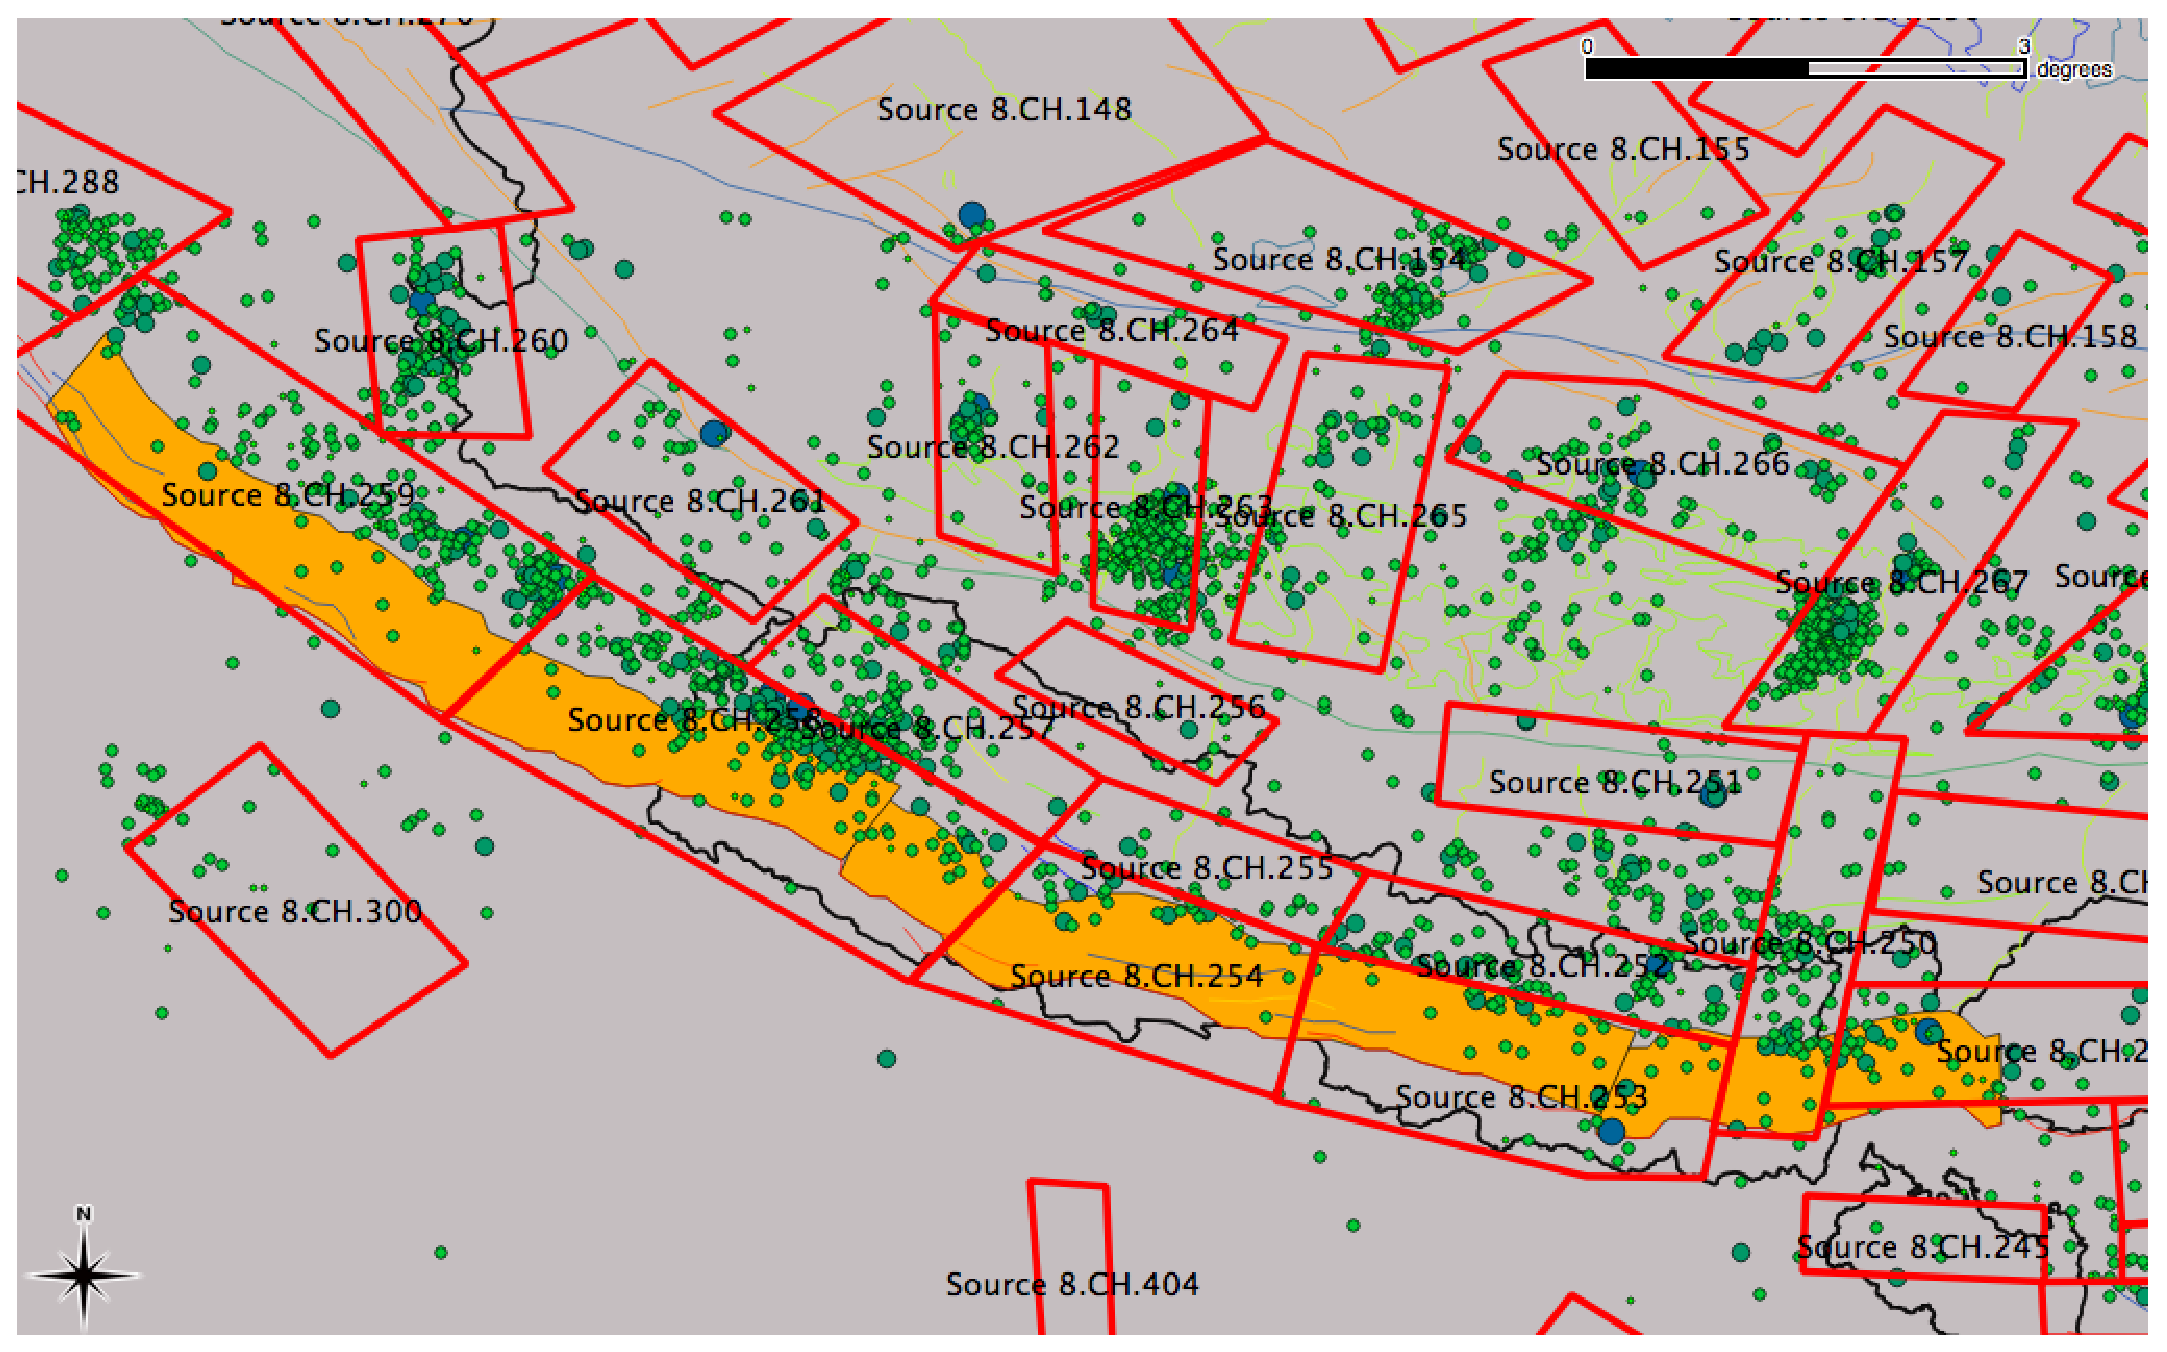
\includegraphics[width=15cm, keepaspectratio=true]{./figures/Kathmandu_plus_GSHAP_sources_labelled.eps}
%	\caption{Seismotectonic Information for Nepal and the Surroundings. Earthquakes catalogue taken from the International Seismological Centre, Area Sources (red) from GSHAP and active fault sources (including surface projections for the Main Boundary Thrust (orange)) from \cite{TaylorYin2009}}
%	\label{fig:KathGSHAPLabel}
%\end{figure}







\cleardoublepage
% % -----------------------------------------------------------------------------
% % -----------------------------------------------------------------------------

\chapter{Seismicity Tools}
\begin{myfancybox}
The objectives of this chapter are:
\begin{itemize}
    \item Describe features of the seismicity tools of the Hazard Modeller's Toolkit 
    \item Run simple calculations using the seismicity tools
\end{itemize}
\end{myfancybox}
  %In the first exercise, the earthquake catalogue will be declustered and the time-variation in completeness analysed. For three of the sources shown in figure \ref{fig:KathGSHAPLabel} (Sources 8.CH.257, 8.CH.258 and 8.CH.259) the recurrence model will be calculated (first using the algorithm of \cite{KijkoSmit2012} - others could be attempted) and maximum magnitude inferred using one of the \cite{Kijko2004} methods 
%
%The configuration file indicates to the toolkit where to look for input files, write output files, which processes and methods to apply and any possible parameters that should be set for given methods. A ''comprehensive'' example of the configuration file is given automatically in the file \verb=config.yml=, which outlines all possible options. The easiest process is to open this file, then edit and delete various options and parameters before saving the configution file to a new file (e.g. \verb=my_config_1.yml=) then executing that in place of the original configuration file.    
%
%The various settings for the different algorithms will be discussed in due course, so the following considers just the main headers (i.e. the control) of the toolkit:
%
%\begin{Verbatim}[frame=single, commandchars=\\\{\}, fontsize=\scriptsize, samepage=false]
%\#*****************************************************************************
%\# HMTK Workflow Configuration File
%\#*****************************************************************************
%
%\#=============================================================================
%\# Input/Output Files
%\#=============================================================================
%
%\# Inputs the Path to the Earthquake Catalogue
%input_catalogue: input/NepalCatalogue_ISC.csv
%\# Inputs the path to the source model (if needed)
%input_model: input/Nepal_3GSHAP_sources.xml
%\# Inputs the path to the output directory
%output_directory: output/
%\# Plotting Folders
%figure_directory: output/plotting/
%
%
%\# Configuration for the Declustering Algorithm (leave blank if not wanted)
%declustering_config: \{\\
%    \# Algorithm choice\\
%    \# 'GardnerKnopoff'  | 'Afteran'\\
%    algorithm: 'GardnerKnopoff',\\
%    \# Choice of magnitude and distance scaling relations\\
%    \# 'GardnerKnopoff' | 'Uhrhammer' | 'Gruenthal'\\
%    time_distance_windows: 'GardnerKnopoff',\\
%    \# Foreshock time as a proportion of aftershock time\\
%    # (GardnerKnopoff only)
%    fs_time_prop: 0.0,\\
%    \# Fixed-width moving time window in days (Afteran only)
%    time_window=60.
%    \}\\
%
%
%\# Configuration for the Completeness Algorithm (only Stepp supported)
%completeness_config: \{
%    \# Choice of algorithm (currently only 'Stepp' supported)
%    algorithm: 'Stepp', 
%    \# Magnitude interval 
%    magnitude_bin: 1.0,
%    \# Time interval (years - as float)
%    time_bin: 5.0,
%    \# Locks the increment to ensure completeness values only increase for
%    \# longer periods 
%    \# True | False
%    increment_lock: True,
%    \# If a plot is wanted (i.e. for Stepp (1971) then set to true
%    include_plot: True,
%    \# If a pre-computed completeness is preferred, define here
%    completeness_table: \}
%
%
%recurrence_config: \{
%    \# Choice of algorithm
%    \# 'Weichert' | 'KijkoSmit' | 'MaxLikelihood'
%    algorithm: 'KijkoSmit',
%    \# Magnitude for calculating rate (if not set will return true a-value
%    reference_magnitude: ,
%    \# Magnitude bin interval
%    magnitude_interval: 0.1,
%    \# Minimum magnitude for sources
%    minimum_magnitude: 4.5\}
%
%
%mmax_config: \{
%    \# Choice of algorithm
%    \# 'KijkoSellevol' | 'KijkoSellevolBayes' | 'KijkoNonparametric | 
%    \# 'CumulativeMoment'
%    algorithm: 'KijkoNonparametric',
%    \# Minimum magniutde (for Kijko & Sellevol methods only)
%    input_mmin: 5.5,
%    \# Input maximum magnitude (if not specified will take largest in catalogue)
%    input_mmax: ,
%    \# Uncertainty on maximum magnitude
%    input_mmax_uncertainty: ,
%    \# Number of N largest earthquakes for consideration (KijkoNonparametric 
%    \# only)
%    number_earthquakes: 50,
%    \# Maximum number of iterations (for all Kijko methods)
%    max_iterations: 1000\}
%       
%\end{Verbatim}
%
%In the initial lines, the toolkit is told the path to look for the input earthquake catalogue (\verb=eq_catalog_file=); the path to which it should write the ''pre-processed catalogue'' (\verb=pprocessing_catalog_file=); the path to which it should write the completeness table, or from which it should read the completeness table if no completeness jobs are defined (\verb=completeness_table_file=); the path from which it should find the area source geometries (\verb=source_model_file=), formatted here as xml (\verb=source_model_file=), and the path to write the output area sources (\verb=result_file=). 
%
%The ''pre-processing'' refers to the combined operations for declustering and/or completeness - i.e. those that remove from consideration all events that are not indicative of complete stationary seismicity. If the user wishes to simply execute those jobs and no others then they should set the value \verb=apply_processing_jobs: no=. This will cause the program to terminate after completion of the pre-processing tasks. If the user has specified a valid path for the \verb=pprocessing_catalog_file= the program will export the catalogue with foreshocks, aftershocks and incomplete magnitude events removed.
%
%After completion of the ''pre-processing'' tasks, the toolkit will then undertake the ''processing'' tasks. These are the calculations to determine the parameters of the double-truncated \cite{GutenbergRichter1944} distribution (i.e. a-value, b-value, minimum magnitude and maximum magnitude). If no source model input is specified in the \verb=source_model_file=, the processing will return (to the screen) a single a-value, b-value, $m_max$ and their respective uncertainties for the whole catalogue. Otherwise the program will loop over each of the zones specified in the file, select those earthquakes from the pre-processed catalogue that are found inside each zone and calculate the recurrence parameters for each zone. The output will then be written to the \verb=result_file=.
%
%\textbf{The order in which the ''pre-processing'' and the ''processing'' tasks are define in the configuration is the order in which the program will execute them!}

\section{The Seismicity Tools}

The seismicity tools are intended for use in deriving activity rates from an observed earthquake catalogue, which may include both instrumental and historical seismicity. The tools are broken down into five separate libraries: i) Declustering, ii) Completeness, iii) Calculation of Gutenberg-Richter a- and b-value, iv) Statistical estimators of maximum magnitude from seismicity) and v) Smoothed Seismicity. In a common use case it is likely that many of the above methods, particularly recurrence and maximum magnitude estimation, may need to be applied to a selected sub-catalogue (e.g. earthquakes within a particular polygon). The toolkit allows for the creation of a source model containing one or more of the supported OpenQuake seismogenic source typologies, which can be used as a reference for selection, e.g. events within an area source (polygon), events within a distance of a fault etc. The supported input formats for both the catalogue and the source model are described below. 

\subsection{The Catalogue Format and Class}

The input catalogue must be formatted as a comma-separated value file (.csv), with the following attributes in the header line (attributes with an * indicate essential attributes), although the order of the columns need not be fixed:

\begin{table}
\begin{tabular}{|l|l|}  \hline 
Attribute & Description \\ \hline
eventID* & A unique identifier (integer) for each earthquake in the catalogue \\
Agency & The code (string) of the recording agency for the event solution  \\
year* & Year of event (integer) in the range -10000 to present \\
 & (events before common era (BCE) should have a negative value)\\
month* & Month of event (integer)\\
day* & Day of event (integer) \\
hour* & Hour of event (integer) - if unknown then set to 0 \\
minute* & Minute of event (integer) - if unknown then set to 0 \\
second* & Second of event (float) - if unknown set to 0.0 \\
timeError & Error in event time (float) \\
longitude* & Longitude of event, in decimal degrees (float) \\
latitude* & Latitude of event, in decimal degrees (float) \\
SemiMajor90 & Length (km) of the semi-major axis of the 90 \% \\
            & confidence ellipsoid for location error (float) \\
SemiMinor90 & Length (km) of the semi-minor axis of the 90 \% \\
            & confidence ellipsoid for location error (float) \\
ErrorStrike & Azimuth (in degrees) of the 90 \% \\
            & confidence ellipsoid for location error (float) \\
depth* & Depth (km) of earthquake (float)\\
depthError & Uncertainty (as standard deviation) in earthquake depth (km) (float)\\
magnitude* & Homogenised magnitude of the event (float) - typically Mw \\
sigmaMagnitude* & Uncertainty on the homogenised magnitude (float) typically Mw \\ \hline
\end{tabular}
\caption{List of Attributes in the Earthquake Catalogue File (* Indicates Essential)}
\label{tab: EQCatalogueFormat}
\end{table}

To load the catalogue using the IPython environment, in an open IPython session type:

\begin{Verbatim}[frame=single, commandchars=\\\{\}, fontsize=\scriptsize, samepage=true]

[1] from hmtk.parsers.catalogue import CsvCatalogueParser

[2] catalogue_filename = 'path/to/catalogue_file.csv'

[3] parser = CsvCatalogueParser(catalogue_filename)

[4] catalogue = parser.read_file()

\end{Verbatim}

\textbf{N.B. the csv file can contain additional attributes of the catalogue too and will be parsed correctly; however, if the attribute is not one that is specifically recognised by the catalogue class then a message will be displayed indicating:}

\begin{Verbatim}[frame=single, commandchars=\\\{\}, fontsize=\scriptsize, samepage=true]
Catalogue Attribute ... is not a recognised catalogue key 
\end{Verbatim}

\textbf{This is expected behaviour and simply indicates that although this data is given in the input file, it is not retained in the data dictionary.}


The variable \verb=catalogue= is an instance of the class hmtk.seismicity.catalogue.Catalogue, which now contains the catalogue itself (as \verb=catalogue.data=) and some methods that can be applied to the catalogue. The first attribute (\verb=catalogue.data=), is a dictionary where each attribute of the catalogue is either a 1-D numpy vector (for float and integer values) or a python list (for string values). For example, to return a vector containing all the magnitudes in the \verb=magnitude= column of the catalogue simply type:

\begin{Verbatim}[frame=single, commandchars=\\\{\}, fontsize=\scriptsize, samepage=true]

In [5]: catalogue.data['magnitude']
Out [e.g.] [5]: array([ 6.5,  6.5,  6. , ...,  4.8,  5.2,  4.1])

\end{Verbatim}

The catalogue class contains several helpful methods (called via \verb=catalogue. ...=):
\begin{itemize}
\item \verb=catalogue.get_number_events()= Returns the number of events currently in the catalogue (integer)

\item \verb=catalogue.load_to_array(keys)= Returns a numpy array of floating data, with the columns ordered according to the list of keys. If the key corresponds to a string item (e.g. Agency) then an error will be raised.

\begin{Verbatim}[frame=single, commandchars=\\\{\}, fontsize=\scriptsize, samepage=true]
In [6]: catalogue.load_to_array(['year', 'longitude', 'latitude', 'depth', 'magnitude'])

Out[6]: 
array([[ 1910.   ,    26.941,    38.507,    13.2  ,     6.5  ],
       [ 1910.   ,    22.19 ,    37.72 ,    20.4  ,     6.5  ],
       [ 1910.   ,    28.881,    33.274,    25.   ,     6.   ],
       ..., 
       [ 2009.   ,    20.054,    39.854,    20.2  ,     4.8  ],
       [ 2009.   ,    23.481,    38.05 ,    15.2  ,     5.2  ],
       [ 2009.   ,    28.959,    34.664,    18.4  ,     4.1  ]]) 
\end{Verbatim}

\item \verb=catalogue.load_from_array(keys, data_array)= Creates the catalogue data dictionary from an array, given header as an ordered list of dictionary keys. This can be used in the case where the earthquake catalogue is loaded in a simple ascii format. For example, if the user wishes to load in a catalogue from the Zmap format, which gives the columns as:

\begin{verbatim}
longitude, latitude, year, month, day, magnitude, depth, hour, 
minute, second
\end{verbatim}

This file type could be parsed into a catalogue without the need of a specific parser, as follows:

\begin{Verbatim}[frame=single, commandchars=\\\{\}, fontsize=\scriptsize, samepage=true]
In [1]: import numpy
# Assuming no headers in the file (set skip_header=1 if headers are found)
In [2]: data = numpy.genfromtxt('PATH/TO/ZMAP_FILE.txt', skip_header=0)

In [3]: headers = ['longitude', 'latitude', 'year', 'month', 'day',
                   'magnitude', 'depth', 'hour', 'minute', 'second']

# Create instance of a catalogue class
In [4]: from hmtk.seismicity.catalogue import Catalogue
In [5]: catalogue = Catalogue()

# Load the data array into the catalogue
In [6]: catalogue.load_from_array(data, headers)

\end{Verbatim}
 

\item \verb=catalogue.get_decimal_time()= Returns the time of the earthquake in a decimal format

\item \verb=catalogue.hypocentres_as_mesh()= Returns the hypocentres of an earthquake as an instance of the openquake.hazardlib.geo.mesh.Mesh class (useful for geospatial functions)

\item \verb=catalogue.hypocentres_to_cartesian()= Returns the hypocentres in a 3D cartesian framework

\item \verb=catalogue.purge_catalogue(flag_vector)= Purges the catalogue of all \verb=False= events in the boolean vector. Thus is used for removing foreshocks and aftershocks from a catalogue after the application of a declustering algorithm.

\item \verb=catalogue.sort_catalogue_chronologically()= Sorts an input into chronological order (N.B. some methods will implicitly assume that the catalogue is in chronological order, so it is recommended to run this function if you believe that there may be events out of order)

\item \verb=catalogue.select_catalogue_events(IDX)= Orders the catalogue according to the event order specified in IDX. Behaves the same as \verb=catalogue.purge_catalogue(IDX)= if IDX is a boolean vector

\item \verb=catalogue.get_depth_distribution(depth_bins, normalisation\=False, bootstrap\=None)= Returns a depth histogram for the catalogue using bins specified by \verb=depth_bins=. If \verb=normalisation\=True= then the function will return the histogram as a probability mass function, otherwise the original count will be returned. If uncertainties are reported on depth such that one or more values in \verb=catalogue.data['depthError']= are greater than 0., the function will perform a bootstrap analysis, taking into account the depth error, with the number of bootstraps given by the keyword \verb=bootstrap=. To generate a simple histogram plot of hypocentral depth, the process below can be followed to produce a depth histogram similar to the one shown in Figure :

\begin{Verbatim}[frame=single, commandchars=\\\{\}, fontsize=\scriptsize, samepage=true]
# Import numpy and matplotlib
In [1]: import numpy as np
In [2]: import matplotlib.pyplot as plt

# Define depth bins for (e.g) 0. - 150 km in intervals of 10 km
In [3]: depth_bins = np.arange(0., 160., 10.)

# Get normalised histograms (without bootstrapping)
In [4]: depth_hist = catalogue.get_depth_distribution(depth_bins, normalisation=True)

# Create a simple histogram plot
In [5]: plt.bar(depth_bins[:-1], depth_hist, width=10.)

# Add some labels
In [6]: plt.xlabel('Depth (km)')
In [7]: plt.ylabel('Density')
\end{Verbatim}


\item \verb=catalogue.get_magnitude_depth_distribution(magnitude_bins, depth_bins, normalisation\=False, bootstrap\=None)= Returns a two-dimensional histogram of magnitude and hypocentral depth, with the corresponding bins defined by the vectors \verb=magnitude_bins= and \verb=depth_bins=. The options \verb=normalisation= and \verb=bootstrap= are the same as for the one dimensional histogram.

\end{itemize}



\subsection{The Source Model Format}

The seismic source model formats currently required by the hmtk are the nrml  The source model is both input and output in GEM's NRML (\verb=Natural Risk Markup Language=) format (although support for shapefile input definitions are expected in future releases). However, unlike the OpenQuake engine, for which each source typology must contain all of the necessary attributes, it is recognised that it may be desirable to use the seismic source model with a partially defined source (one for which only the ID, name and geometry are known) in order to make use of the modelling tools. Therefore, the validation checks have been relaxed to allow for data such as the recurrence model, the hypocentral depth distribution and the faulting mechanism to be specified at a later stage. However, if using this minimal format it will not be possible to use the resulting output file in OpenQuake until the remaining information is filled in.  

A full description of the complete nrml seismogenic source model format is found in the OpenQuake Version 1.0 manual \cite{crowley2010}. An example of a minimal format is shown below for:

\subsubsection{Point Source}

\begin{Verbatim}[frame=single, commandchars=\\\{\}, fontsize=\scriptsize, samepage=true]

<?xml version='1.0' encoding='utf-8'?>
<nrml xmlns:gml="http://www.opengis.net/gml" xmlns="http://openquake.org/xmlns/nrml/0.4">
    <sourceModel name="Some Source Model">
        <pointSource id="2" name="point" tectonicRegion="">

        <pointGeometry>
            <gml:Point>
                <gml:pos>-122.0 38.0</gml:pos>
            </gml:Point>

            <upperSeismoDepth>0.0</upperSeismoDepth>
            <lowerSeismoDepth>10.0</lowerSeismoDepth>
        </pointGeometry>

        <magScaleRel></magScaleRel>
        <ruptAspectRatio></ruptAspectRatio>

        <truncGutenbergRichterMFD aValue="" bValue="" minMag="" maxMag="" />

        <nodalPlaneDist>
            <nodalPlane probability="" strike="" dip="" rake="" />
            <nodalPlane probability="" strike="" dip="" rake="" />
        </nodalPlaneDist>

        <hypoDepthDist>
            <hypoDepth probability="" depth="" />
            <hypoDepth probability="" depth="" />
        </hypoDepthDist>

    </pointSource>
    </sourceModel>
</nrml>

\end{Verbatim}


\subsubsection{Area Source}

\begin{Verbatim}[frame=single, commandchars=\\\{\}, fontsize=\scriptsize, samepage=true]

<?xml version='1.0' encoding='utf-8'?>
<nrml xmlns:gml="http://www.opengis.net/gml" xmlns="http://openquake.org/xmlns/nrml/0.4">

<sourceModel name="Some Source Model">
    <!-- Note: Area sources are identical to point sources, except for the geometry. -->
    <areaSource id="1" name="Quito" tectonicRegion="">
        <areaGeometry>
            <gml:Polygon>
                <gml:exterior>
                    <gml:LinearRing>
                        <gml:posList>
                         -122.5 38.0
                         -122.0 38.5
                         -121.5 38.0
                         -122.0 37.5
                        </gml:posList>
                    </gml:LinearRing>
                </gml:exterior>
            </gml:Polygon>

            <upperSeismoDepth>0.0</upperSeismoDepth>
            <lowerSeismoDepth>10.0</lowerSeismoDepth>
        </areaGeometry>

        <magScaleRel></magScaleRel>

        <ruptAspectRatio></ruptAspectRatio>

        <incrementalMFD minMag="" binWidth="">
            <occurRates></occurRates>
        </incrementalMFD>

        <nodalPlaneDist>
            <nodalPlane probability="" strike="" dip="" rake="" />
            <nodalPlane probability="" strike="" dip="" rake="" />
        </nodalPlaneDist>

        <hypoDepthDist>
            <hypoDepth probability="" depth="" />
            <hypoDepth probability="" depth="" />
        </hypoDepthDist>

    </areaSource>
    </sourceModel>
</nrml>

\end{Verbatim}

\subsubsection{Simple Fault Source}

\begin{Verbatim}[frame=single, commandchars=\\\{\}, fontsize=\scriptsize, samepage=true]

<?xml version='1.0' encoding='utf-8'?>
<nrml xmlns:gml="http://www.opengis.net/gml" xmlns="http://openquake.org/xmlns/nrml/0.4">
    <sourceModel name="Some Source Model">
        <simpleFaultSource id="3" name="Mount Diablo Thrust" tectonicRegion="">

            <simpleFaultGeometry>
                <gml:LineString>
                    <gml:posList>
                        -121.82290 37.73010
                        -122.03880 37.87710
                    </gml:posList>
                </gml:LineString>

                <dip>45.0</dip>
                <upperSeismoDepth>10.0</upperSeismoDepth>
                <lowerSeismoDepth>20.0</lowerSeismoDepth>
            </simpleFaultGeometry>

            <magScaleRel></magScaleRel>

            <ruptAspectRatio></ruptAspectRatio>

            <incrementalMFD minMag="" binWidth="">
                <occurRates></occurRates>
            </incrementalMFD>

            <rake></rake>
        </simpleFaultSource>
    </sourceModel>
</nrml>

\end{Verbatim}


\subsubsection{Complex Fault Source}

\begin{Verbatim}[frame=single, commandchars=\\\{\}, fontsize=\scriptsize, samepage=true]

<?xml version='1.0' encoding='utf-8'?>
<nrml xmlns:gml="http://www.opengis.net/gml" xmlns="http://openquake.org/xmlns/nrml/0.4">
    <sourceModel name="Some Source Model">
    <complexFaultSource id="4" name="Cascadia Megathrust" tectonicRegion="">

        <complexFaultGeometry>
            <faultTopEdge>
                <gml:LineString>
                    <gml:posList>
                        -124.704 40.363 0.5493260E+01
                        -124.977 41.214 0.4988560E+01
                        -125.140 42.096 0.4897340E+01
                    </gml:posList>
                </gml:LineString>
            </faultTopEdge>

            <intermediateEdge>
                <gml:LineString>
                    <gml:posList>
                        -124.704 40.363 0.5593260E+01
                        -124.977 41.214 0.5088560E+01
                        -125.140 42.096 0.4997340E+01
                    </gml:posList>
                </gml:LineString>
            </intermediateEdge>

            <intermediateEdge>
                <gml:LineString>
                    <gml:posList>
                        -124.704 40.363 0.5693260E+01
                        -124.977 41.214 0.5188560E+01
                        -125.140 42.096 0.5097340E+01
                    </gml:posList>
                </gml:LineString>
            </intermediateEdge>

            <faultBottomEdge>
                <gml:LineString>
                    <gml:posList>
                        -123.829 40.347 0.2038490E+02
                        -124.137 41.218 0.1741390E+02
                        -124.252 42.115 0.1752740E+02
                    </gml:posList>
                </gml:LineString>
            </faultBottomEdge>
        </complexFaultGeometry>

        <magScaleRel></magScaleRel>
        
        <ruptAspectRatio></ruptAspectRatio>

        <truncGutenbergRichterMFD aValue="" bValue="" minMag="" maxMag="" />

        <rake></rake>
    </complexFaultSource>
    </sourceModel>
</nrml>

\end{Verbatim}

To load in a source model such as those shown above, in an IPython environment simply execute the following:

\begin{Verbatim}[frame=single, commandchars=\\\{\}, fontsize=\scriptsize, samepage=true]

In: [1] from hmtk.parsers.source_model.nrml04_parser import nrmlSourceModelParser

In: [2] model_filename = 'path/to/source_model_file.xml'

In: [3] model_parser = nrmlSourceModelParser(model_filename)

In: [4] model = model_parser.read_file()
Area source - ID: 1, name: Quito
Point Source - ID: 2, name: point
Simple Fault source - ID: 3, name: Mount Diablo Thrust
Complex Fault Source - ID: 4, name: Cascadia Megathrust

\end{Verbatim}

If loaded successfully a list of the source typology, ID and source name for each source will be returned to the screen as shown above. The variable \verb=model= contains the whole source model, and can support multiple typologies (i.e. point, area, simple fault and complex fault).


\section{Declustering}

To identify Poissonian rate of seismicity, it is necessary to remove foreshocks/aftershocks/swarms from the catalogue. The Modeller's Toolkit contains, at present, two algorithms to undertake this task, with more under development.

\subsection{\cite{GardnerKnopoff1974}}

The most widely applied simple windowing algorithm is that of 
\cite{GardnerKnopoff1974}. Originally conceived for Southern California, 
the method simply identifies aftershocks by virtue of fixed time-distance
windows proportional to the magnitude of the main shock. Whilst this 
premise is relatively simple, the manner in which the windows are 
applied can be ambiguous. Four different possibilities can be 
considered (\cite{LuenStark2012}):

\begin{enumerate}
\item Search events in magnitude-descending order. Remove events if it is 
    in the window of the largest event
\item Remove every event that is inside the window of a previous event, 
    including larger events
\item An event is in a cluster if, and only if, it is in the window of at 
    least one other event in the cluster. In every cluster remove all 
    events except the largest
\item In chronological order, if the $i^{th}$ event is in the window of a 
    preceding larger shock that has not already been deleted, remove it. 
    If a larger shock is in the window of the $i^{th}$ event, delete the 
    $i^{th}$ event. Otherwise retain the $i^{th}$ event.
\end{enumerate}

It is the first of the four options that is implemented in the current 
toolkit, whilst others may be considered in future.  The algorithm is 
capable if identifying foreshocks and aftershocks, simply by applying 
the windows forward and backward in time from the mainshock. 
No distinction is made between primary aftershocks (those resulting 
from the mainshock) and secondary or tertiary aftershocks (those 
originating due to the previous aftershocks); however, it is assumed 
all would occur within the window.

Several modifications to the time and distance windows have been 
suggested, which are summarised in \cite{vanStiphout2012}. The windows 
originally suggested by \cite{GardnerKnopoff1974} are approximated by:

\begin{equation}\begin{split} 
\mbox{distance (km)} = &10^{0.1238 M + 0.983}\\
\mbox{time (decimal years)} = & 
\begin{cases} 10^{0.032 M + 2.7389} & \text{if $M \geq 6.5$} \\ 
              10^{0.5409 M - 0.547} & \mbox{otherwise}  \end{cases}\end{split}
\end{equation}

An alternative formulation is proposed by Gr\"unthal (as reported in\cite{vanStiphout2012}):

\begin{equation}\begin{split} 
\mbox{distance (km)} = & e^{1.77 + \left( {0.037 + 1.02 M} \right)^2} \\ 
   \mbox{time (decimal years)} = & \begin{cases}   |e^{-3.95+ \left( {0.62 + 17.32 M}
    \right)^2}|    & \text{if $M \geq 6.5$ } \\ 10^{2.8 + 0.024 M} & 
    \text{otherwise}  \end{cases}\end{split}
\end{equation}
A further alternative is suggested by \cite{Uhrhammer1986}
%
\begin{equation}
\mbox{distance (km)} = e^{-1.024 + 0.804 M} \quad \mbox{time (decimal years)} = 
    e^{-2.87 + 1.235 M}
\end{equation}

A comparison of the expected window sizes with magnitude are shown for 
distance  and time (Figure \ref{fig:declust_scaling}).

\begin{figure}[htb]
  \centering
  \begin{subcaption}
      \centering
      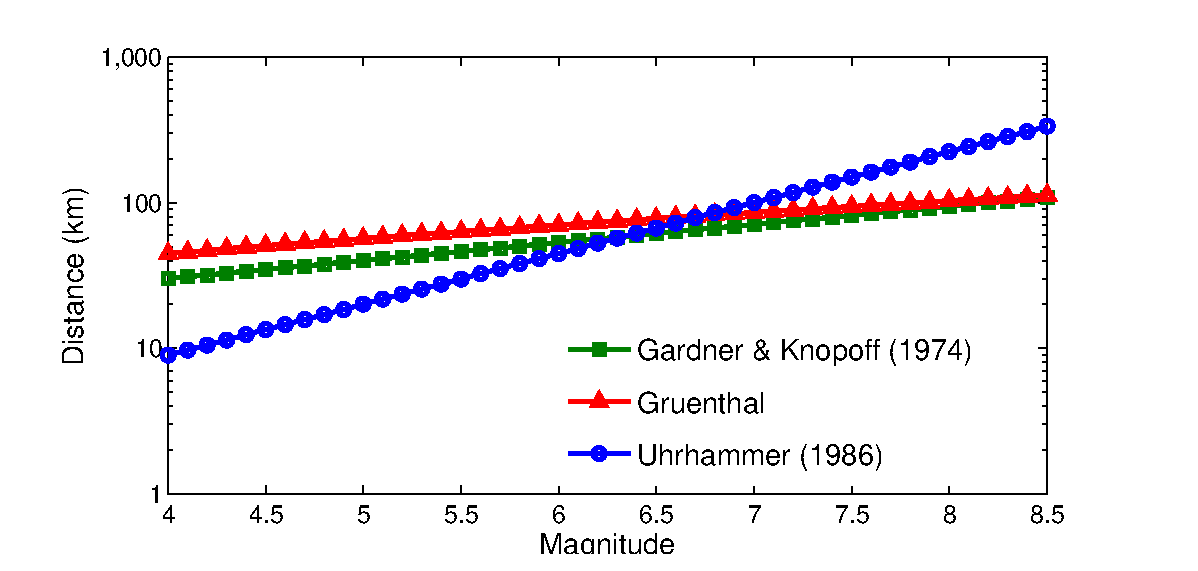
\includegraphics[width=8cm]{./figures/declustering_distance_windows.eps}
	\end{subcaption}
  \begin{subcaption}
      \centering
      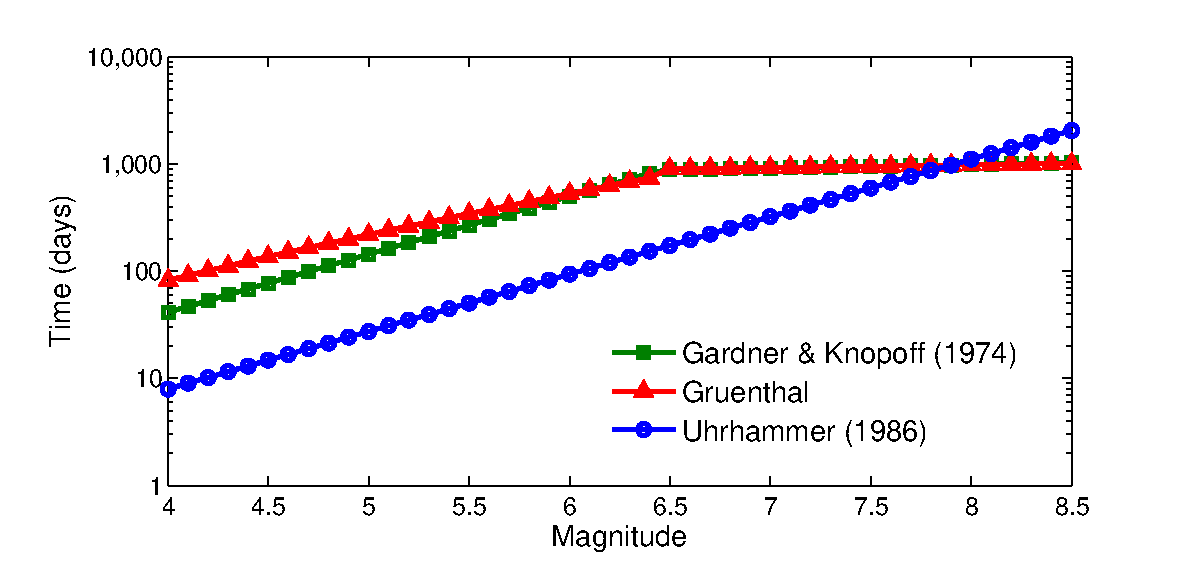
\includegraphics[width=8cm]{./figures/declustering_time_windows.eps}
	\end{subcaption}	
	\caption{Scaling of declustering time and distance windows with magnitude}
	\label{fig:declust_scaling}
\end{figure}

The \cite{GardnerKnopoff1974} algorithm and its derivatives represent 
are most computationally straightforward approach to declustering. The \verb=time_dist_windows= attribute indicates the choice of the 
time and distance window scaling model from the three listed. As 
the current version of this algorithm considers the events in a 
descending-magnitude order, the parameter \verb=foreshock_time_window= 
defines the size of the time window used for searching for foreshocks, 
as a fractional proportion of the size of the aftershock window (the 
distance windows are always equal for both fore- and aftershocks). 
So for an evenly sized time window for foreshocks and aftershocks, 
\verb=foreshock_time_window= should equal 1. For shorter or longer 
foreshock time windows this parameter can be reduced or increased respectively.

To run a declustering analysis on the earthquake catalogue it is necessary to set-up the configuration using a python dictionary.\footnote{A dictionary is Python's way of storing a mapping of data (including different types) to a set of keys (similar to a data structure in Matlab).} A config file for the \cite{GardnerKnopoff1974} algorithm, using for example the \cite{Uhrhammer1986} time-distance windows with equal sized time window for aftershocks and foreshocks, would be created as shown:

\begin{Verbatim}[frame=single, commandchars=\\\{\}, fontsize=\scriptsize, samepage=true]

In [1]: from hmtk.seismicity.declusterer.distance_time_windows import UhrhammerWindow

In [2]: declust_config = \{'time_distance_window': UhrhammerWindow(),
   ....:                   'fs_time_prop': 1.0\}

\end{Verbatim}


To run the declustering algorithm simply import and run the algorithm as shown:

\begin{Verbatim}[frame=single, commandchars=\\\{\}, fontsize=\scriptsize, samepage=true]

In [1]: from hmtk.seismicity.declusterer.distance_time_windows import UhrhammerWindow

In [2]: declust_config = \{'time_distance_window': UhrhammerWindow(),
   ....:                   'fs_time_prop': 1.0\}

\end{Verbatim}


\begin{Verbatim}[frame=single, commandchars=\\\{\}, fontsize=\scriptsize, samepage=true]

In [3]: from hmtk.seismicity.declusterer.dec_gardner_knopoff import GardnerKnopoffType1

In [4]: declustering = GardnerKnopoffType1()

In [5]: cluster_index, cluster_flag = declustering.decluster(catalogue,
                                                             declust_config)

\end{Verbatim}

There are two outputs of a declustering algorithm: \verb=cluster_index= and \verb=cluster_flag=. Both are numpy vectors, of the same length as the catalogue, containing information about the clusters in the catalogue. \verb=cluster_index= indicates the cluster to which each event is assigned (0 if not assigned to a cluster). \verb=cluster_flag= indicates whether an event is a non-Poissonian event, in which case the value is assigned to 1, or a mainshock, the value is assigned as 0. This output definition is the same for all declustering algorithms.

At this point the user may wish to either retain the catalogue in its current format, in which case they may wish to add on the clustering information into another attribute of the catalogue.data dictionary, or they may wish to purge the catalogue of non-Poissonian events. 

To simply add the clustering information to the data dictionary simply type:

\begin{Verbatim}[frame=single, commandchars=\\\{\}, fontsize=\scriptsize, samepage=true]

In [6]: catalogue.data['Cluster_Index'] = cluster_index
In [7]: catalogue.data['Cluster_Flag'] = cluster_flag

\end{Verbatim}
 
Alternatively, to purge the catalogue of non-Poissonian events:

\begin{Verbatim}[frame=single, commandchars=\\\{\}, fontsize=\scriptsize, samepage=true]

In [6]: mainshock_flag = cluster_flag == 0
In [7]: catalogue.purge_catalogue(mainshock_flag)

\end{Verbatim}


\subsection{AFTERAN (\cite{Musson1999PSHABalkan})}

A particular development of the standard windowing approach is introduced in the program AFTERAN \cite{Musson1999PSHABalkan}. This is a modification of the \cite{GardnerKnopoff1974} algorithm, using a moving time window rather than a fixed time window. In AFTERAN, considering each earthquake in order of descending magnitude, events within a fixed distance window are identified (the distance window being those suggested previously). These events are searched using a moving time window of T days. For a given mainshock, non Poissonian events are identified if they occur both within the distance window and the initial time window. The time window is then moved, beginning at the last flagged event, and the process repeated. For a given mainshock, all non-Poissonian events are identified when the algorithm finds a continuous period of T days in which no aftershock or foreshock is identified. 

The theory of the AFTERAN algorithm is broadly consistent with that of \cite{GardnerKnopoff1974}. This algorithm, whilst a little more computationally complex, and therefore slower, than the \cite{GardnerKnopoff1974} windowing approach, remains simple to implement. 

As with the \cite{GardnerKnopoff1974} function, the \verb=time_dist_window= attribute indicates the choice of the time and distance window scaling model. The parameter \verb=time_window= indicates the size (in days) of the moving time window used to identify fore- and aftershocks. The following example will show how to run the AFTERAN algorithm, using the  \cite{GardnerKnopoff1974} definition of the distance windows, and a fixed-width moving time window of 100 days.

  
\begin{Verbatim}[frame=single, commandchars=\\\{\}, fontsize=\scriptsize, samepage=true]

In [1] from hmtk.seismicity.declusterer.dec_afteran import Afteran

In [2]: from hmtk.seismicity.declusterer.distance_time_windows import GardnerKnopoffWindow   
 
In [3]: declust_config = \{'time_distance_window': GardnerKnopoffWindow(),
                          'time_window': 100.0\} 

In [4]: declustering = Afteran()

In [5]: cluster_index, cluster_flag = declustering.decluster(catalogue, declust_config)

\end{Verbatim}

 

%::::::::::::::::::::::::::::::::::::::::::::::::::::::::::::::::::::::::::::::::::::::::::::::::::::::::::::::::::::::::::::::::::::::::::::::::::::::::::::::

\section{Completeness}

In the earliest stages of processing an instrumental seismic catalogue to derive inputs for seismic hazard analysis, it is necessary to determine the magnitude completeness threshold of the catalogue. To outline the meaning of the term ''magnitude completeness'' and the requirements for its analysis as an input to PSHA, the terminology of \cite{MignanWoessner2012} is adopted. This defines the magnitude of completeness as the ''lowest magnitude at which 100 \% of the events in a space-time volume are detected (\cite{RydelekSacks1989, WoessnerWiemer2005})''. Incompleteness of an earthquake catalogue will produce bias when determining models of earthquake recurrence, which may have a significant impact on the estimation of hazard at a site. Identification of the completeness magnitude of an earthquake catalogue is therefore a clear requirement for the processing of input data for seismic hazard analysis.

It should be noted that this summary of methodologies for estimating completeness is directed toward techniques that can be applied to a ''typical'' instrumental seismic catalogue. We therefore make the assumption that the input data will contain basic information for each earthquake such as time, location, magnitude. We do not make the assumption that network-specific or station-specific properties (e.g., configuration, phase picks, attenuation factors) are known a priori. This limits the selection of methodologies to those classed as estimators of ''sample completeness'', which defines completeness on the basis of the statistical properties of the earthquake catalogue, rather than ''probability-based completeness'', which defines the probability of detection given knowledge of the properties of the seismic network (\cite{SchorlemmerWoessner2008}). This therefore excludes the methodology of (\cite{SchorlemmerWoessner2008}), and similar approaches such as that of \cite{Felzer2008}

The current workflows assume that completeness will be applied to the whole catalogue, ideally returning a table of time-varying completeness. The option to explore spatial variation in completeness is not explicitly supported, but could be accommodated by an appropriate configuration of the toolkit.

In the current version (July 2013) of the Modeller's Toolkit only the \cite{Stepp1971} methodology for analysis of catalogue completeness is implemented. Further methods are in development, and will be input in future releases.

%\subsection{User-defined Table}
%
%This is simply a filtering that will remove from further consideration any events outside of the completeness bounds defined by the user. The table represents the time variation in $M_C$ and can be input as a separate file (in comma-separated value format) in the following format.
%\begin{Verbatim}[frame=single, commandchars=\\\{\}, fontsize=\scriptsize]
%1990.0, 4.0\\
%1960.0, 5.0\\
%1900.0, 6.0\\
%1700.0, 7.0\\
%\end{Verbatim}
%
%The left-hand column represents the earliest year at which the earthquake is complete at the corresponding magnitude in the right-hand column. \\
%\textbf{Important: The values in the completeness file must be entered from most-recent to oldest!} 

\subsection{\cite{Stepp1971}}

This is one of the earliest analytical approaches to estimation of completeness magnitude. It is based on estimators of the mean rate of recurrence of earthquakes within given magnitude and time ranges, identifying the completeness magnitude when the observed rate of earthquakes above MC begins to deviate from the expected rate. If a time interval ($T_i$) is taken, and the earthquake sequence assumed Poissonian, then the unbiased estimate of the mean rate of events per unit time interval of a given sample is:

\begin{equation}
   \lambda = \frac{1}{n} \sum_{i = 1}^{n} T_i
\end{equation}

with variance $\sigma_{\lambda}^{2} = \lambda / n$. Taking the unit time interval to be 1 year, the standard deviation of the estimate of the mean is:

\begin{equation}
   \sigma_{\lambda} = \sqrt{\lambda} / \sqrt{T}
\end{equation}

where $T$ is the sample length. As the Poisson assumption implies a stationary process, $\sigma_{\lambda}$ behaves as $1/\sqrt{T}$ in the sub-interval of the sample in which the mean rate of occurrence of a magnitude class is constant. Time variation of $M_C$ can usually be inferred graphically from the analysis, as is illustrated in Figure \ref{fig:SteppFigExample1}. In this example, the deviation from the $1/\sqrt{T}$ line for each magnitude class occurs at around 40 years  for $4.5 < M < 5$, 100 years for $5.0  < M < 6.0$, approximately 150 years for $6.0 < M < 6.5$ and 300 years for $M > 6.5$. Knowledge of the sources of earthquake information for a given catalogue may usually be reconciled with the completeness time intervals.

\begin{figure}[htb]
	\centering
		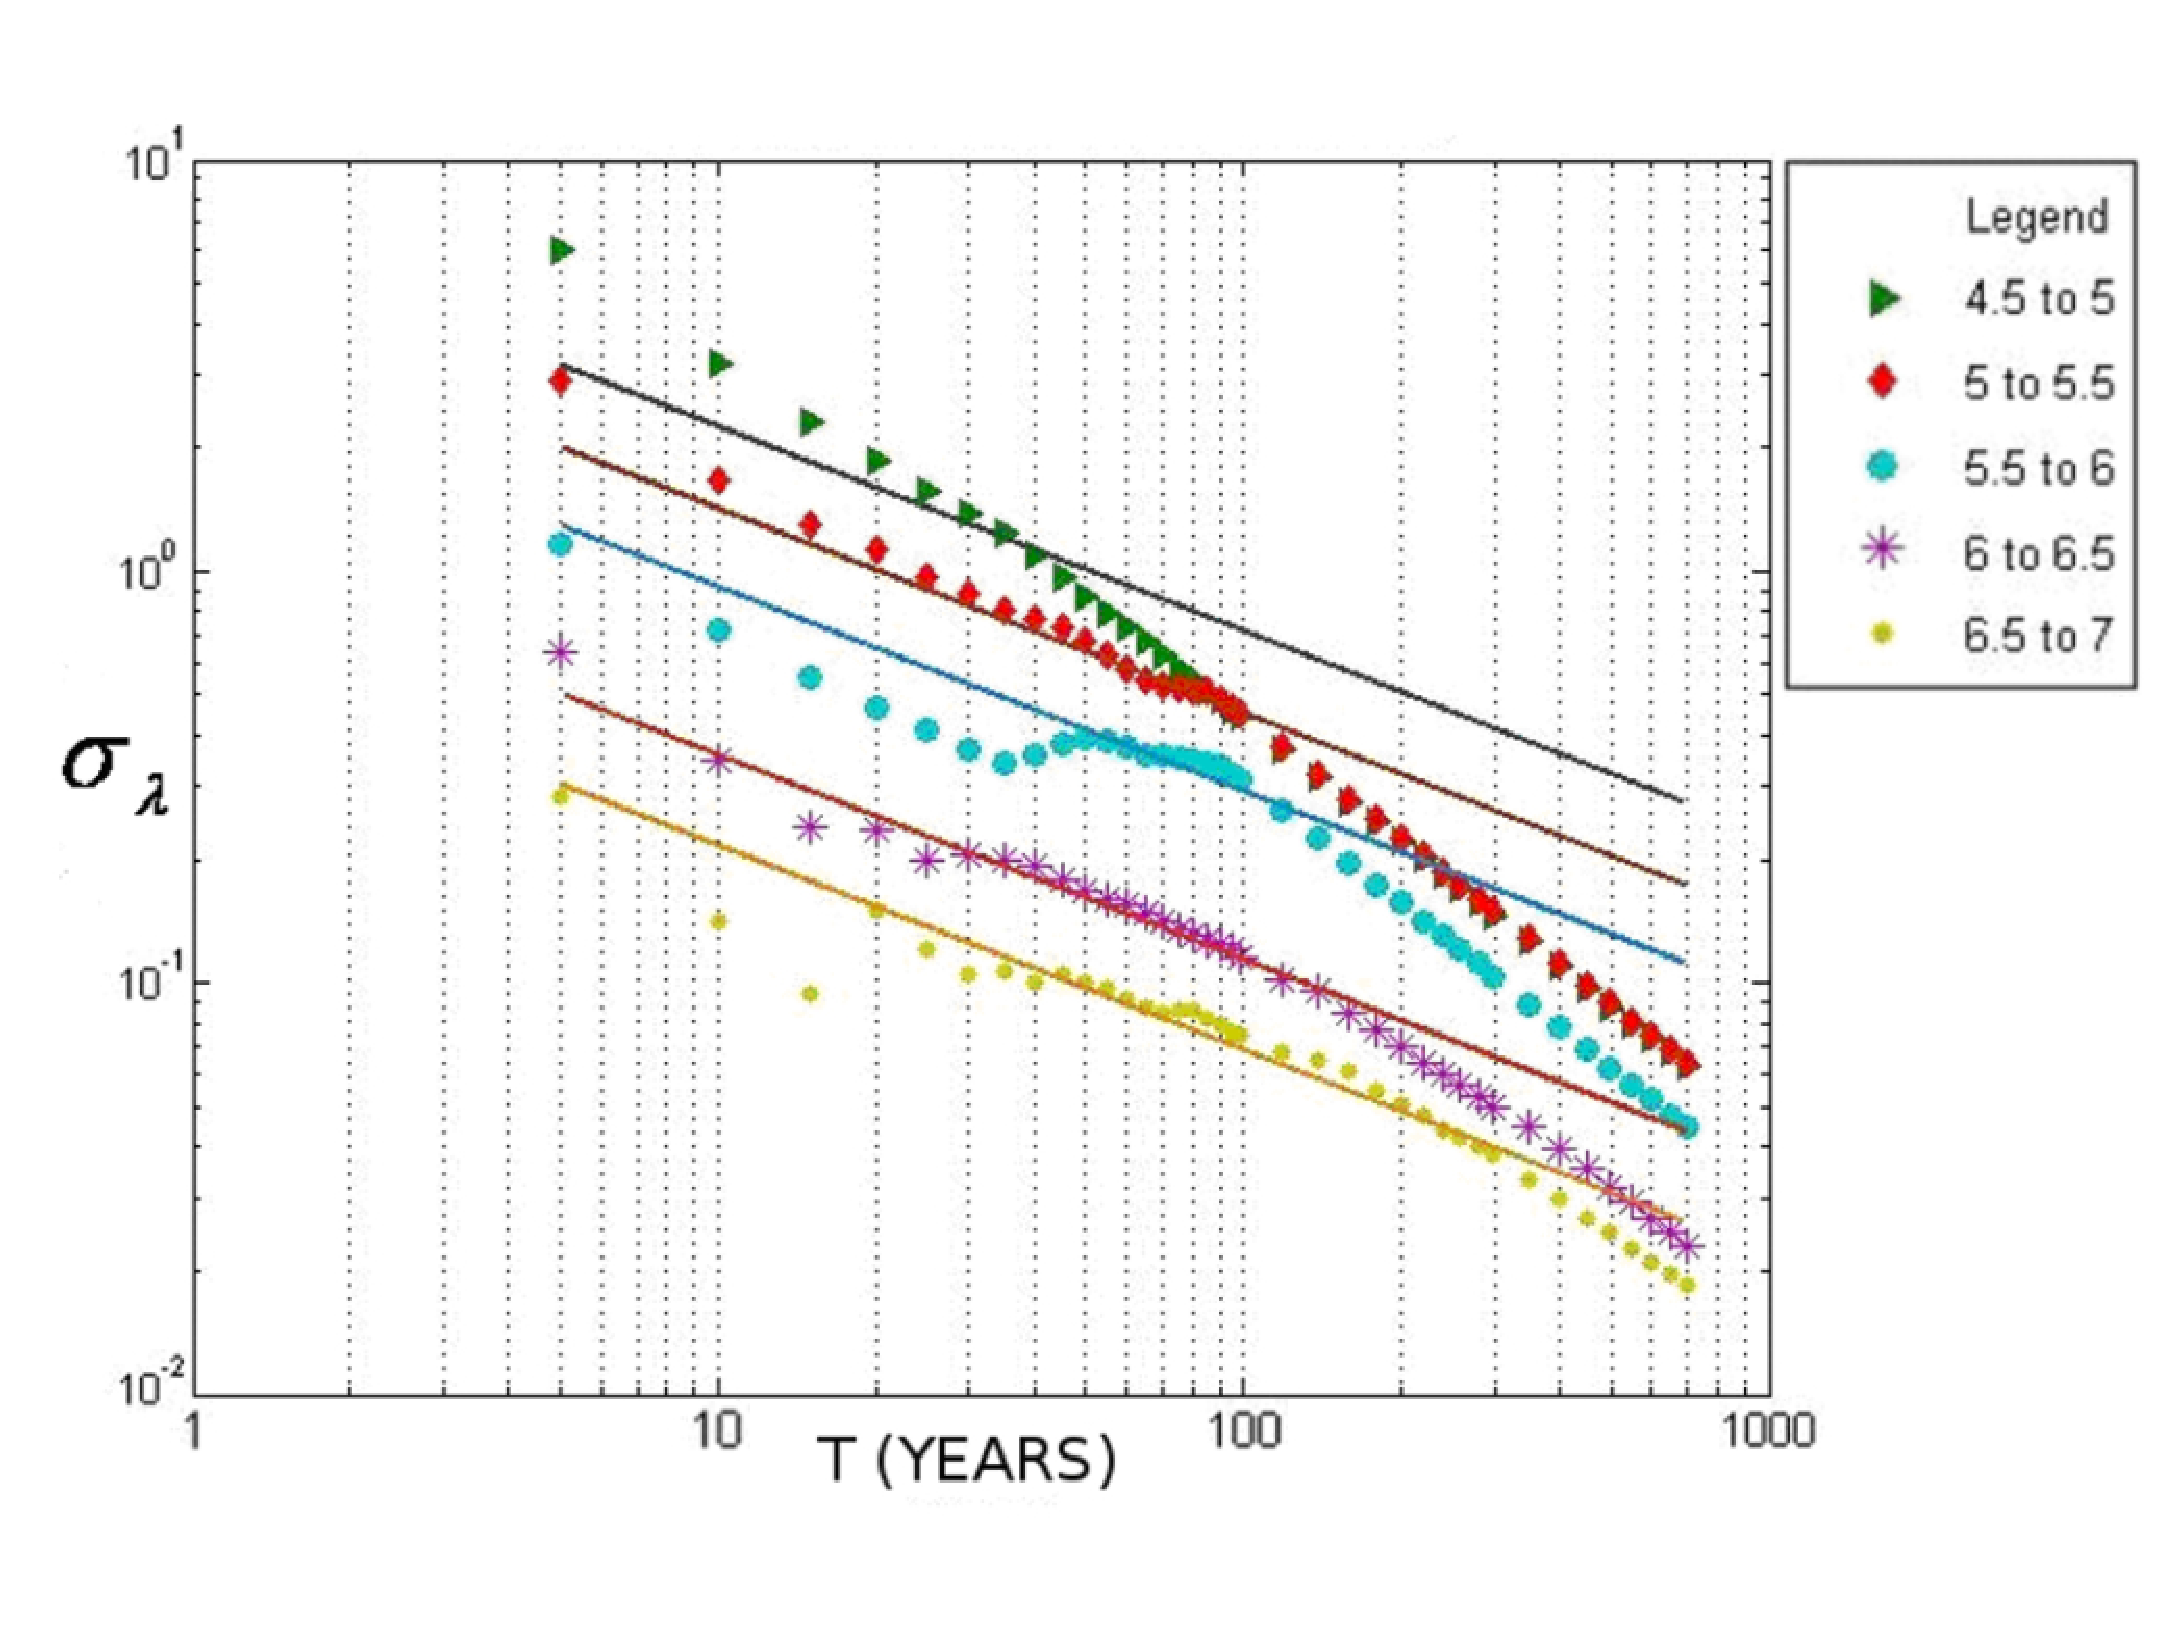
\includegraphics[height=10cm, keepaspectratio=true]{./figures/C2Fig1SteppFig1.eps}
	\caption{Example of Completeness Estimation by the \cite{Stepp1971} methodology}
	\label{fig:SteppFigExample1}
\end{figure}

The analysis of \citet{Stepp1971} is a coarse, but relatively robust, approach to estimating the temporal variation in completeness of a catalogue. It has been widely applied since its development. The accuracy of the completeness magnitude depends on the magnitude and time intervals considered, and a degree of judgement is often needed to determine the time at which the rate deviates from the expected values. It has tended to be applied to catalogues on a large scale, and for relatively higher completeness magnitudes. 

To translate the methodology from a largely graphical methods into a computational method the completeness period needs to be identified by automatically identifying the point at which the gradient of the observed values decreases with respect to that expected from a Poisson process (see \ref{fig:SteppFigExample1}). In the implementation found within the current toolkit, the divergence point is identified by fitting a two-segment piecewise linear function to the observed data. Although a two-segment piecewise linear function is normally fit with four parameters (intercept, $slope_1$, $slope_2$ and crossover point), by virtue of the assumption that for the complete catalogue the rate is assumed to be stationary such that $\sigma_{\lambda} = \frac{1}{\sqrt{T}}$ the slope of the first segment can be fixed as $-0.5$, and the second slope should be constrained such that $slope_2 \leq -0.5$, whilst the crossover point ($x_c$) is subject to the constraint ($x_c \geq 0.0$). Thus it is possible to fit the two-segment linear function using constrained optimisation with only three free parameters. For this purpose the toolkit minimises the residual sum-of-squares of the model fit using numerical optimisation. 

To run the \cite{Stepp1971} algorithm the configuration parameters should be entered in the form of a dictionary, such as the example shown below:

\begin{Verbatim}[frame=single, commandchars=\\\{\}, fontsize=\scriptsize, samepage=true]

In [1]: comp_config = \{'magnitude_bin': 0.5,
                        'time_bin': 5.,
                        'increment_lock': True\}

\end{Verbatim}

The algorithm has three configurable options. The \verb=time_bin= parameter describes the size of the time window in years, the \verb=magnitude_bin= parameter describes the size of the magnitude bin, sensitivity is as described previously. The final option (\verb=increment_lock=) is an option that is used to ensure consistency in the results to avoid the completeness magnitude increasing for the latest intervals in the catalogue simply due to the variability associated with the short duration. If \verb=increment_lock= is set to \verb=True=, the program will ensure that the completeness magnitude for shorter, more recent windows is less than or equal to that of older, longer windows. This is often a condition for some recurrence analysis tools, so it may be advisable to set this option to true in certain workflows. Otherwise it should be set to \verb=False to show the apparent variability=. Some degree of judgement is necessary here. In particular it is expected that the user may be aware of circumstances particular to their catalogue for which a recent increase in completeness magnitude is expected (for example, a certain recording network no longer operational).  


The process of running the algorithm is shown below:

\begin{Verbatim}[frame=single, commandchars=\\\{\}, fontsize=\scriptsize, samepage=true]

In [2]: from hmtk.seismicity.completeness.comp_stepp_1971 import Stepp1971

In [3]: completeness_algorithm = Stepp1971()

In [4]: completeness_table = completeness_algorithm.completeness(catalogue, comp_config)

In [5]: completeness_table
Out[5]: 
array([[ 1990.  ,     4.25],
       [ 1962.  ,     4.75],
       [ 1959.  ,     5.25],
       [ 1906.  ,     5.75],
       [ 1906.  ,     6.25],
       [ 1904.  ,     6.75],
       [ 1904.  ,     7.25]])

\end{Verbatim}

As shown in the resulting \verb=completeness_table=, the completeness algorithm will output the time variation in completeness (in this example with the \verb=increment_lock= set) in the form of a two-column table with column 1 indicating the completeness year for the magnitude bin centred on the magnitude value found in column 2.


At present, it may be the case that the user wishes to enter a time-varying completeness results for use in subsequent functions, based on alternative methods or on judgement. This can be entered in the \verb=completeness_table= setting, as in the example shown here (take note of the requirements for the square brackets):

\begin{Verbatim}[frame=single, commandchars=\\\{\}, fontsize=\scriptsize]

completeness_table: [[1990., 4.0],
                     [1960., 5.0],
                     [1930., 6.0],
                     [1900., 6.5]]

\end{Verbatim}

If a \verb=completeness_table= is input then this will override the selection of the completeness algorithm, and the calculation will take the values in \verb=completeness_table= directly. 

%::::::::::::::::::::::::::::::::::::::::::::::::::::::::::::::::::::::::::::::::::::::::::::::::::::::::::::::::::::::::::::::::::::::::::::::::::::::::::::::

\section{Recurrence Models}

The current sets of tools are intended to determine the parameters of the \cite{GutenbergRichter1944} recurrence model, namely the a- and b-value. It is expected that in the most common use case the catalogue that is input to these algorithms will be declustered, with a time-varying completeness defined according to a \verb=completeness_table= of the kind shown previously. If no \verb=completeness_table= is input the algorithm will assume the input catalogue is complete above the minimum magnitude for its full duration.

\subsection{\cite{Aki1965}}

The classical maximum likelihood estimator for a simple unbounded \cite{GutenbergRichter1944} model is that of \cite{Aki1965}, adapted for binned magnitude data by \cite{Bender1983}. It assumes a fixed completeness magnitude ($M_C$) for the catalogue, and a simple power law recurrence model. It does not explicitly take into account magnitude uncertainty.

\begin{equation}
   b = \frac{ \log_{10} \left( e \right)}{ \bar{m} - m_0 + \left( {\frac{\Delta M}{2}} \right)}
\end{equation}

\noindent where $\bar{m}$ is the mean magnitude, $m_0$ the minimum magnitude and $\Delta M$ the discretisation interval of magnitude within a given sample.

\subsection{Maximum Likelihood}

This method adjusts the \cite{Aki1965} and \cite{Bender1983} method to incorporate for time variation in completeness. The catalogue is divided into
into S sub-catalogues, where each sub-catalogue corresponds to a period 
with a corresponding $M_C$.  An average a- and b-value (with uncertainty) is returned by taking 
the mean of the a- and b-value of each sub-catalogue, weighted by 
the number of events in each sub-catalogue.

\begin{equation}
   \hat{b} = \frac{1}{S} \sum_{i = 1}^{S} w_i b_i
\end{equation}

\begin{Verbatim}[frame=single, commandchars=\\\{\}, fontsize=\scriptsize]

In [1]: mle_config = \{'magnitude_interval': 0.1,
                      'Average Type': 'Weighted',
                      'reference_magnitude': None\}

In [2]: from hmtk.seismicity.occurrence.b_maximum_likelihood import BMaxLikelihood

In [3]: recurrence = BMaxLikelihood()

In [4]: bval, sigmab, aval, sigmaa = recurrence.calculate(catalogue, mle_config, 
    completeness=completeness_table)

\end{Verbatim}

Where \verb=magnitude_window= indicates the size of the magnitude bin, \verb=recurrence_algorithm= and \verb=reference_magnitude= the magnitude for which the output calculates that rate greater than or equal to (set to \verb=0= for $10^{a}$). 

\subsection{\cite{KijkoSmit2012}}

A recent adaption of the \cite{Aki1965} estimator of b-value for  a catalogue containing different completeness periods has been proposed by \cite{KijkoSmit2012}. Dividing the earthquake catalogue into $s$ subcatalogues of $n_i$ events with corresponding completeness magnitudes $m_{c_i}$ for $i = 1, 2, ..., s$, the likelihood function of $\beta$ where $\beta = b \ln		 \left( {10.0} \right)$ is given as:

\begin{equation}
    \mathbf{L} = \prod_{i = 1}^{s} \prod_{j = 1}^{n_i} \beta \exp(\left[ {-\beta \left( {m_j^i - m_{min}^i } \right) } \right])
\end{equation}

which gives a maximum likelihood estimator of $\beta$:

\begin{equation}
    \beta = \left( {\frac{r_1}{\beta_1} + \frac{r_2}{\beta_2} + \dots + \frac{r_s}{\beta_s}} \right)^{-1}
\end{equation}

where $r_i = n_i / n$ and $n = \sum_{i = 1}^{s} n_i$ above the level of completeness $m_i$.

\begin{Verbatim}[frame=single, commandchars=\\\{\}, fontsize=\scriptsize]

In [1]: kijko_smit_config = \{'magnitude_interval': 0.1,
                             'reference_magnitude': None\}

\end{Verbatim}

\subsection{\cite{Weichert1980}}

Recognising the typical conditions of an earthquake catalogue, \cite{Weichert1980} developed a maximum likelihood estimator of $b$ for grouped magnitudes and unequal periods of observation. The likelihood formulation for this approach is:

\begin{equation}
   \mathbf{L} \left( {\beta | n_i, m_i, t_i} \right) = \frac{ N!}{\prod_i n_i!} \prod_i p_{i}^{n_i}
\end{equation}

where $\mathbf{L}$ is the likelihood estimator of $\beta$, $n$ the number of earthquakes in magnitude bin m with observation period t. The parameter $p$ is defined as:

\begin{equation}
   p_i = \frac{t_i \exp \left( {-\beta m_i} \right) }{\sum_j t_j \exp \left( {-\beta m_j} \right)}
\end{equation}

The extremum of $\ln \left( {\mathbf{L}}\right)$ is found at:

\begin{equation} 
   \frac{\sum_i t_i m_i \exp \left( {-\beta m_i} \right)}{\sum_j t_j \exp \left( {-\beta m_j} \right)}
\end{equation}

The computational implementation of this method is given as an appendix to \cite{Weichert1980}. This formulation of the maximum likelihood estimator for b-value, and consequently seismicity rate, is in widespread use, with applications in many national seismic hazard analysis \citep[e.g.]{usgsNSHM1996,usgsNSHM2002}. The algorithm has been demonstrated to be efficient and unbiased for most applications. It is recognised by \citet{Felzer2008} that an implicit assumption is made regarding the stationarity of the seismicity for all the time periods. 

To implement the \cite{Weichert1980} recurrence estimator, the configuration properties are defined as:

\begin{Verbatim}[frame=single, commandchars=\\\{\}, fontsize=\scriptsize]

In [1]: weichert_config = \{`magnitude_interval': 0.1,
                           `reference_magnitude': None,
                           \# The remaining parameters are optional
                           `bvalue': 1.0,
                           `itstab': 1E-5,
                           `maxiter': 1000\}

\end{Verbatim}

As the \cite{Weichert1980} algorithm is reaches the MLE estimation by iteration then three additional optional parameters can control the iteration process: \verb=bvalue= is the initial guess for the b-value, \verb=itstab= the difference in b-value in order to reach convergence, and \verb=maxiter= the maximum number of iterations. \footnote{The iterative nature of the \cite{Weichert1980} algorithm can result in very slow convergence and unstable behaviour when the magnitudes infer b-values that are very small, or even negative. This can occur when very few events are in the resulting catalogue, or when the magnitudes converge within a narrow range.}



%::::::::::::::::::::::::::::::::::::::::::::::::::::::::::::::::::::::::::::::::::::::::::::::::::::::::::::::::::::::::::::::::::::::::::::::::::::::::::::::
\section{Maximum Magnitude}

The estimation of the maximum magnitude for use in seismic hazard analysis is a complex, and often controversial, process that should be guided by information from geology and the seismotectonics of a seismic source. Estimation of maximim magnitude from the observed (instrumental and historical) seismicity can be undertaken using methods assuming a truncated \cite{GutenbergRichter1944} model, or via non-parametric methods that are independent any assumed functional form. 

\subsection{\cite{Kijko2004}}

Three different estimators of maximum magnitude are given by \cite{Kijko2004}, each depending on a different set of assumptions:
\begin{enumerate}
\item ''Fixed b-value'': Assumes a single b-value with no uncertainty 
\item ''Uncertain b-value'': Assumes and uncertain b-value defined by an expected b and the standard deviation
\item ''Non-Parametric Gaussian'': Assumes no functional form (can be applied to seismicity observed to follow a more characteristic distribution)
\end{enumerate}

Each of these estimators assumes the general form:

\begin{equation}
m_{max} = m_{max}^{obs} + \Delta
\end{equation}

where $\Delta$ is an increment that is dependent on the estimator used.

The uncertainty on $m_{max}$ is also defined according to:

\begin{equation}
    \sigma_{m_{max}} = \sqrt{\sigma_{m_{max}^{obs}}^2 + \Delta^{2}}
\end{equation}

In the three estimators some lower bound magnitude constraint must be defined. For those estimators that assume an exponential recurrence model the lower bound magnitude must be specified by the users. For the non-Parametric Gaussian method and explicit lower bound magnitude does not have to be specified; however, the estimation is conditioned upon the largest N magnitudes, where N must be specified by the user.

If the user wishes to input a maximum magnitude that is larger than that observed in the catalogue (e.g. a known historical magnitude), this can be specified in the config file using \verb=input_mmax= with the corresponding uncertainty defined by \verb=input_mmax_uncertainty=. If these are not defined (i.e. set to \verb=None=) then the maximum magnitude will be taken from the catalogue.

All three estimators require an iterative solution, therefore additional parameters can be specified in the configuration file that control the iteration process: \verb=tolerance= difference in $M_Max$ estimate for the algorithm to be considered converged, and \verb=maximum_iterations= the maximum number of iterations for stability. 


\subsubsection{''Fixed b-value''}

For a catalogue of $n$ earthquakes, whose magnitudes are distributed by a \cite{GutenbergRichter1944} distribiution with a fixed "b" value, the increment of maximum magnitude is determined via:

\begin{equation}
\Delta = \int\limits_{m_{min}} ^{m_{max}} \left[ {\frac{1 - \exp \left[ {-\beta \left( {m - m_{min}} \right)} \right]}{1 - \exp \left[ {-\beta \left( {m_{max}^{obs} - m_{min}} \right) } \right]}} \right] ^n dm
\end{equation}


The execution of the \cite{Kijko2004} ''fixed-b'' algorithm is as follows:

\begin{Verbatim}[frame=single, commandchars=\\\{\}, fontsize=\scriptsize]

In [1]: mmax_config = \{`input_mmax': 7.6,
                       `input_mmax_uncertainty': 0.22,
                       `b-value': 1.0,
                       `input_mmin': 5.0,
                       `tolerance': 1.0E-5,  \# Defaults to this if not specified
                       `maximum_iterations': 1000\} \# Defaults to this if not specified
                       
In [2]: from hmtk.seismicity.max_magnitude.kijko_sellevol_fixed_b import KijkoSellevolFixedb

In [3]: mmax_estimator = KijkoSellevolFixedb()

In [4]: mmax, mmax_uncertainty = mmax_estimator.get_mmax(catalogue, mmax_config)
                
\end{Verbatim}

\subsubsection{''Uncertain b-value''}

For a catalogue of $n$ earthquakes, whose magnitudes are distributed by a \cite{GutenbergRichter1944} distribiution with an uncertain "b" value, characterised by and expected term ($b$) and a corresponding undertainty ($\sigma_b$), the increment of maximum magnitude is determined via:


\begin{equation}
\Delta = \left( {C_{\beta}} \right)^n \int\limits_{m_min}^{m_max} \left[ {1 - \left( {\frac{p}{p + m - m_{min}}} \right) ^q} \right]^n dm
\end{equation}

where $\beta = b \ln \left( {10.0} \right)$, $p = \beta / \left( {\sigma_{\beta}} \right) ^ 2$, $q = \left( {\beta / \sigma_{\beta}} \right) ^ 2$ and $C_{\beta}$ is a normalising coefficient determined via:

\begin{equation}
C_{\beta} = \frac{1}{1 - \left[ {p / \left( {p + m_{max} - m_{min}} \right) } \right]^q}
\end{equation}

In both the fixed and uncertain ''b'' case a minimum magnitude will need to be input into the calculation. If this value is lower than the minimum magnitude observed in the catalogue the iterator may not stabilise to a satisfactory value, so it is recommended to use a minimum magnitude that is greater than the minimum found in the observed catalogue.

The execution of the ''uncertain b-value'' estimator is undertaken in a very similar to that of the fixed b-value, the only additional parameter being the \verb=sigma-b= term:

\begin{Verbatim}[frame=single, commandchars=\\\{\}, fontsize=\scriptsize]

In [1]: mmax_config = \{'input_mmax': 7.6,
                       'input_mmax_uncertainty': 0.22,
                       'b-value': 1.0,
                       'sigma-b': 0.15
                       'input_mmin': 5.0,
                       'tolerance': 1.0E-5, \# Defaults to this if not specified
                       'maximum_iterations': 1000\} \# Defaults to this if not specified
                       
In [2]: from hmtk.seismicity.max-magnitude.kijko_sellevol_bayes import KijkoSellevolBayes

In [3]: mmax_estimator = KijkoSellevolBayes()

In [4]: mmax, mmax_uncertainty = mmax_estimator.get_mmax(catalogue, mmax_config)
                
\end{Verbatim}

\subsubsection{Non-Parametric Gaussian}

The non-parametric Gaussian estimator for maximum magnitude $m_{max}$ is defined as:

\begin{equation}
\Delta = \int\limits_{m_{min}}^{m_{max}} \left[ {\frac{\sum_{i = 1}^{n} \left[ {\Phi \left( {\frac{m - m_i}{h}} \right) - \Phi \left( {\frac{m_{min} - m_i}{h}} \right)} \right]}{\sum_{i = 1}^{n} \left[ {\Phi \left( {\frac{m_{max} - m_i}{h}} \right) - \Phi \left( {\frac{m_{min} - m_i}{h}} \right)} \right]}} \right]^n  dm
\end{equation}
where $m_{min}$ and $m_{max}$ are the minimum and maximum magnitudes from a set of $n$ events, $\Phi$ is the standard normal cumulative distribution function. $h$ a kernel smoothing factor:
\begin{equation}
h = 0.9 \times min\left( {\sigma, IQR / 1.34} \right) \times n^{-1 / 5}
\end{equation}
with $\sigma$ the standard deviation of a set of n earthquakes with magnitude $m_{i}$ where $i = 1, 2, ... n$, and $IQR$ the inter-quartile range. 

Therefore the uncertainty on $m_{max}$ is conditioned primarily on the uncertainty of the largest observed magnitude. As in many catalogues the largest observed magnitude may be an earlier historical event, which will be associated with a large uncertainty, this estimator tends towards large uncertainties on $m_{max}$.

Due to the need to define some additional parameters the configuration file is slightly different. No b-value or minimum magnitude needs to be specified; however, the algorithm will consider only the largest \verb=number_earthquakes= magnitudes (or all magnitudes if the number of observations is smaller). The algorithm also numerically approximates the integral of the Gaussian pdf, so \verb=number_samples= is the number of samples of the distribution. The rest of the execution remains the same as for the exponential recurrence estimators of $M_{max}$:

\begin{Verbatim}[frame=single, commandchars=\\\{\}, fontsize=\scriptsize]

In [1]: mmax_config = \{'input_mmax': 7.6,
                       'input_mmax_uncertainty': 0.22,
                       'number_samples': 51, \# Default value
                       'number_earthquakes': 100 \# Default value
                       'tolerance': 1.0E-5, \# Defaults to this if not specified
                       'maximum_iterations': 1000\} \# Defaults to this if not specified
                       
In [2]: from hmtk.seismicity.max-magnitude.kijko_nonparametric_gausian import KijkoNonParametricGaussian

In [3]: mmax_estimator = KijkoNonParametricGaussian()

In [4]: mmax, mmax_uncertainty = mmax_estimator.get_mmax(catalogue, mmax_config)
                
\end{Verbatim}


\subsection{Cumulative Moment\citep{MakropoulosBurton1983}}

The cumulative moment release method is an adaptation of the cumulative strain energy release method for estimating $m_{max}$ originally proposed by \cite{MakropoulosBurton1983}. Another method based on a pseudo-graphical formulation, an estimator of maximum magnitude can be derived from a plot of cumulative seismic moment release with time. The average slope of this plot indicates the mean moment release for the input catalogue in question. Two further straight lines are defined with gradients equal to that of the slope of mean cumulative moment release, both enveloping the cumulative plot. The vertical distance between these two lines indicates the total amount of moment that may be released in the region, if no earthquakes were to occur in the corresponding time (i.e. the distance between the upper and lower bounding lines on the time axis). This concept is illustrated in Figure \ref{fig:Cumulative_Moment}. 

\begin{figure}[htb]
	\centering
		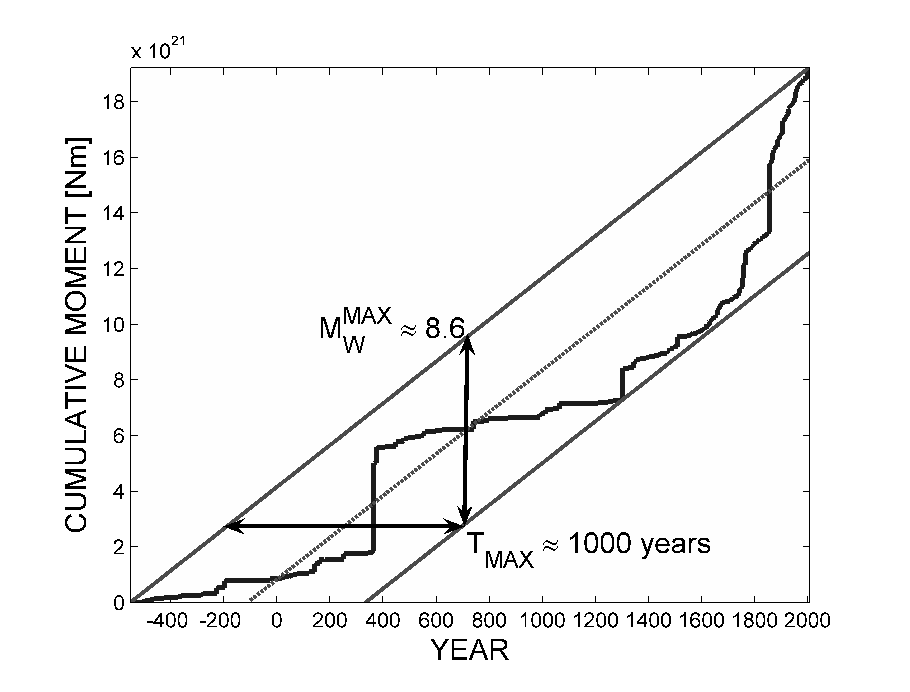
\includegraphics[height=6cm, keepaspectratio=true]{./figures/Cumulative_Moment.eps}
	\caption{Illustratation of Cumulative Moment Release Concept}
	\label{fig:Cumulative_Moment}
\end{figure}

The cumulative moment estimator of $m_{max}$, whilst simple in concept, has several key advantages. As a non-parametric method it is independent of any assumed probability distribution and cannot estimate $m_{max}$ lower than the observed $m_{max}$. It is also principally controlled by the largest events in the catalogue, this making it relative insensitive to uncertainties in completeness or lower bound threshold. In practice, this estimator, and to some extent that of \cite{Kijko2004} are dependent on having a sufficiently long record of events relative to the strain cycle for the region in question, such that the estimate of average moment release is stable. This will obviously depend on the length of the catalogue, and for some regions, particularly those in low strain intraplate environments, it is often the case that $m_{max}$ will be close to the observed $m_{max}$. Therefore it may be the case that it is most appropriate to use these techniques on a larger scale, either considering multiple sources or an appropriate tectonic proxy.

For the cumulative moment estimator it is possible to take into account the uncertainty on $m_{max}$ by applying bootstrap sampling to the observed magnitudes and their respective uncertainties. This has the advantage that $\sigma_{m_{max}}$ is not controlled by the uncertainty on the observed $m_{max}$, as it is for the \cite{Kijko2004} algorithm. Instead it takes into account the uncertainty on all the magnitudes in the catalogue. The cost of this, however, is that this method is more computationally intensive, and therefore slower, than \cite{Kijko2004}, depending on the number of bootstrap samples the user chooses.

The algorithm is slightly simpler to run than the \cite{Kijko2004} methods; however, due to the bootstrapping process it is slightly slower. It is run as per the following example:

\begin{Verbatim}[frame=single, commandchars=\\\{\}, fontsize=\scriptsize]

In [1]: mmax_config = {'number_bootstraps': 1000}
                       
In [2]: from hmtk.seismicity.max_magnitude.cumulative_moment_release import CumulativeMoment

In [3]: mmax_estimator = CumulativeMoment()

In [4]: mmax, mmax_uncertainty = mmax_estimator.get_mmax(catalogue, mmax_config)
                
\end{Verbatim}

For the cumulative moment algorithm the only user configurable parameter is the \verb=number_bootstraps=, which is the number of samples used during the bootstrapping process. 

\section{Smoothed Seismicity}

The use of smoothed seismicity in seismic hazard analysis has generally become a common way of characterising distributed seismicity, for which the seismogenic source are defined exclusively from the uncertain locations of observed seismicity. There are many different methods for smoothing the catalogue, adopting different smoothing kernels or making different correction factors to compensate for spatial and/or temporal completeness. 

\subsection{\cite{frankel1995}}

A smoothed seismicity method that has one of the clearest precedents for use in seismic hazard analysis is that of \cite{frankel1995}, originally derived to characterise the seismicity of the Central and Eastern United States as part of the 1996 National Seismic Hazard Maps of the United States. The method applies a simple isotropic Gaussian smoothing kernel to derive the expected rate of events at each cell $\tilde{n}_i$ from the observed rate $n_j$ of seismicity in a grid of $j$ cells. This kernel takes the form:

\begin{equation}
\tilde{n_i} = \frac{\sum_j n_j e^{d_{ij}^2 / c^2}}{\sum_j e^{d_{ij}^2 / c^2}} 
\end{equation}

In the implementation of the algorithm, two steps are taken that we prefer to make configurable options here. The first step is that the time-varying completeness is accounted for using a correction factor ($t_f$) based on the \cite{Weichert1980} method:

 \begin{equation}
 t_f = \frac{\sum_i e^{-\beta m_{c_i}}}{\sum_i T_i e^{-\beta m_{c_i}}} 
 \end{equation}
 
where $m_{c_i}$ the completeness magnitude corresponding to the mid-point of each completeness interval, and $T_i$ the duration of the completeness interval. The completeness magnitude bins must be evenly-spaced; hence, within the application of the progress a function is executed to render the input completeness table to one in which the magnitudes are evenly spaced with a width of 0.1 magnitude units. 

\subsection{Implementing the Smoothed Seismicity Analysis}

The smoothed seismicity separates out the core implementation (i.e. the gridding, counting and execution of the code) and the choice of kernel. An example of the execution process is as follows:

The first stage is to upload the catalogue into an instance of the catalogue class

\begin{Verbatim}[frame=single, commandchars=\\\{\}, fontsize=\scriptsize]

In [1]: input_file = 'path/to/input_file.csv'

In [2]: from hmtk.parsers.catalogue.csv_catalogue_parser import CsvCatalogueParser

In [3]: parser = CsvCatalogueParser(input_file)

In [4]: catalogue = parser.read_file()

\end{Verbatim}

Next setup the smoothing algorithm using and the corresponding kernel:

\begin{Verbatim}[frame=single, commandchars=\\\{\}, fontsize=\scriptsize]

# Imports the smoothed seismicity algorithm
In [5]: from hmtk.seismicity.smoothing.smoothed_seismicity import SmoothedSeismicity

# Imports the Kernel function
In [6]: from hmtk.seismicity.smoothing.kernels.isotropic_gaussian import IsotropicGaussian

# Grid limits should be set up as 
# [min_long, max_long, spc_long, min_lat max_lat, spc_lat, min_depth, max_depth,
# spc_depth]
In [7]: grid_limits = [0., 10., 0.1, 0., 10., 0.1, 0., 60., 30.]
# Assuming a b-value of 1.0
In [8]: smooth_seis = SmoothedSeismicity(grid_limits, use_3d=True, bvalue=1.0)

\end{Verbatim}

The smoothed seismicity function needs to be set up with three variables: i) the extent (and spacing) of the grid, ii) the choice to use 3D smoothing (i.e. distances are taken as hypocentral rather than epicentral) and iii) the input b-value. The extent of the grid can also be defined from the catalogue. If preferred the user need only specify the spacing of the longitude-latitude grid (as a single floating point value), then the grid will be defined by taking the bounding box of the earthquake catalogue and extended by the total smoothing length (i.e. the bandwidth (in km) multiplied by the maximum number of bandwidths). 

To run the smoothed seismicity analysis, the configurable parameters are: \verb=BandWidth= the bandwidth of the Gaussian kernel (in km), \verb=Length_Limit= the number of bandwidths considered as a maximum smoothing length, and \verb=increment= chooses whether to output the incremental a-value (for consistency with the original \cite{frankel1995} methodology) or the cumulative a-value (corresponding to the a-value of the Gutenberg-Richter model).


The algorithm requires two essential inputs (the earthquake catalogue and the config file), and three optional inputs:

\begin{itemize}
\item \verb=completeness_table= A table of completeness magnitudes and their corresponding completeness years (as output from the completeness algorithms)

\item \verb=smoothing_kernel= An instance of the required smoothing
kernel class (currently only Isotropic Gaussian is supported - and will be used if not specified)

\item \verb=end_year= The final year of the catalogue. This will be taken as the last year found in the catalogue, if not specified by the user
\end{itemize}

The analysis is then run via:

\begin{Verbatim}[frame=single, commandchars=\\\{\}, fontsize=\scriptsize]
# Set up config (e.g. 50 km band width, up to 3 bandwidths)
In [9]: config = {`Length_Limit': 3., `BandWidth': 50., 'increment': True}

# Run the analysis!
In [10]: output_data = smooth_seis.run_analysis(catalogue, config, completeness_table, smoothing_kernel=IsotropicGaussian(), end_year=None)

# To write the resulting data to a csv file
In [11] = smooth_seis.write_to_csv(`path/to/output_file.csv')
\end{Verbatim}

The resulting output will be a csv file with the following columns:
\begin{Verbatim}[frame=single, commandchars=\\\{\}, fontsize=\scriptsize]
Longitude, Latitude, Depth, Observed Count, Smoothed Rate, b-value
\end{Verbatim}

\noindent where \verb=Observed Count= is the observed number of earthquakes in each cell, and \\ 
\verb=Smoothed Rate= is the smoothed seismicity rate.








\cleardoublepage


% \cleardoublepage
% %
\chapter{Hazard Tools}
\begin{myfancybox}
The objectives of this chapter are:
\begin{itemize}
    \item Introduction to the HMTK source model classes
    \item Understand how to link source models to seismicity
    \item Run simple PSHA calculations in OpenQuake, using the HMTK
\end{itemize}
\end{myfancybox}
  \section{Source Model and Hazard Tools}

\subsection{The Source Model Format}

The seismic source model formats currently required by the hmtk are the nrml  The source model is both input and output in GEM's NRML (``Natural Risk Markup Language``) format (although support for shapefile input definitions are expected in future releases). However, unlike the OpenQuake engine, for which each source typology must contain all of the necessary attributes, it is recognised that it may be desirable to use the seismic source model with a partially defined source (one for which only the ID, name and geometry are known) in order to make use of the modelling tools. Therefore, the validation checks have been relaxed to allow for data such as the recurrence model, the hypocentral depth distribution and the faulting mechanism to be specified at a later stage. However, if using this minimal format it will not be possible to use the resulting output file in OpenQuake until the remaining information is filled in.  

A full description of the complete nrml seismogenic source model format is found in the OpenQuake Version 1.0 manual \parencite{crowley2010}. An example of a minimal format is shown below for:

\subsubsection{Point Source}

\begin{Verbatim}[frame=single, commandchars=\\\{\}, fontsize=\scriptsize]

<?xml version='1.0' encoding='utf-8'?>
<nrml xmlns:gml="http://www.opengis.net/gml" xmlns="http://openquake.org/xmlns/nrml/0.4">
    <sourceModel name="Some Source Model">
        <pointSource id="2" name="point" tectonicRegion="">

        <pointGeometry>
            <gml:Point>
                <gml:pos>-122.0 38.0</gml:pos>
            </gml:Point>

            <upperSeismoDepth>0.0</upperSeismoDepth>
            <lowerSeismoDepth>10.0</lowerSeismoDepth>
        </pointGeometry>

        <magScaleRel></magScaleRel>
        <ruptAspectRatio></ruptAspectRatio>

        <truncGutenbergRichterMFD aValue="" bValue="" minMag="" maxMag="" />

        <nodalPlaneDist>
            <nodalPlane probability="" strike="" dip="" rake="" />
            <nodalPlane probability="" strike="" dip="" rake="" />
        </nodalPlaneDist>

        <hypoDepthDist>
            <hypoDepth probability="" depth="" />
            <hypoDepth probability="" depth="" />
        </hypoDepthDist>

    </pointSource>
    </sourceModel>
</nrml>

\end{Verbatim}


\subsubsection{Area Source}

\begin{Verbatim}[frame=single, commandchars=\\\{\}, fontsize=\scriptsize]

<?xml version='1.0' encoding='utf-8'?>
<nrml xmlns:gml="http://www.opengis.net/gml" xmlns="http://openquake.org/xmlns/nrml/0.4">

<sourceModel name="Some Source Model">
    <!-- Note: Area sources are identical to point sources, except for the geometry. -->
    <areaSource id="1" name="Quito" tectonicRegion="">
        <areaGeometry>
            <gml:Polygon>
                <gml:exterior>
                    <gml:LinearRing>
                        <gml:posList>
                         -122.5 38.0
                         -122.0 38.5
                         -121.5 38.0
                         -122.0 37.5
                        </gml:posList>
                    </gml:LinearRing>
                </gml:exterior>
            </gml:Polygon>

            <upperSeismoDepth>0.0</upperSeismoDepth>
            <lowerSeismoDepth>10.0</lowerSeismoDepth>
        </areaGeometry>

        <magScaleRel></magScaleRel>

        <ruptAspectRatio></ruptAspectRatio>

        <incrementalMFD minMag="" binWidth="">
            <occurRates></occurRates>
        </incrementalMFD>

        <nodalPlaneDist>
            <nodalPlane probability="" strike="" dip="" rake="" />
            <nodalPlane probability="" strike="" dip="" rake="" />
        </nodalPlaneDist>

        <hypoDepthDist>
            <hypoDepth probability="" depth="" />
            <hypoDepth probability="" depth="" />
        </hypoDepthDist>

    </areaSource>
    </sourceModel>
</nrml>

\end{Verbatim}

\subsubsection{Simple Fault Source}

\begin{Verbatim}[frame=single, commandchars=\\\{\}, fontsize=\scriptsize]

<?xml version='1.0' encoding='utf-8'?>
<nrml xmlns:gml="http://www.opengis.net/gml" xmlns="http://openquake.org/xmlns/nrml/0.4">
    <sourceModel name="Some Source Model">
        <simpleFaultSource id="3" name="Mount Diablo Thrust" tectonicRegion="">

            <simpleFaultGeometry>
                <gml:LineString>
                    <gml:posList>
                        -121.82290 37.73010
                        -122.03880 37.87710
                    </gml:posList>
                </gml:LineString>

                <dip>45.0</dip>
                <upperSeismoDepth>10.0</upperSeismoDepth>
                <lowerSeismoDepth>20.0</lowerSeismoDepth>
            </simpleFaultGeometry>

            <magScaleRel></magScaleRel>

            <ruptAspectRatio></ruptAspectRatio>

            <incrementalMFD minMag="" binWidth="">
                <occurRates></occurRates>
            </incrementalMFD>

            <rake></rake>
        </simpleFaultSource>
    </sourceModel>
</nrml>

\end{Verbatim}


\subsubsection{Complex Fault Source}

\begin{Verbatim}[frame=single, commandchars=\\\{\}, fontsize=\scriptsize]

<?xml version='1.0' encoding='utf-8'?>
<nrml xmlns:gml="http://www.opengis.net/gml" xmlns="http://openquake.org/xmlns/nrml/0.4">
    <sourceModel name="Some Source Model">
    <complexFaultSource id="4" name="Cascadia Megathrust" tectonicRegion="">

        <complexFaultGeometry>
            <faultTopEdge>
                <gml:LineString>
                    <gml:posList>
                        -124.704 40.363 0.5493260E+01
                        -124.977 41.214 0.4988560E+01
                        -125.140 42.096 0.4897340E+01
                    </gml:posList>
                </gml:LineString>
            </faultTopEdge>

            <intermediateEdge>
                <gml:LineString>
                    <gml:posList>
                        -124.704 40.363 0.5593260E+01
                        -124.977 41.214 0.5088560E+01
                        -125.140 42.096 0.4997340E+01
                    </gml:posList>
                </gml:LineString>
            </intermediateEdge>

            <intermediateEdge>
                <gml:LineString>
                    <gml:posList>
                        -124.704 40.363 0.5693260E+01
                        -124.977 41.214 0.5188560E+01
                        -125.140 42.096 0.5097340E+01
                    </gml:posList>
                </gml:LineString>
            </intermediateEdge>

            <faultBottomEdge>
                <gml:LineString>
                    <gml:posList>
                        -123.829 40.347 0.2038490E+02
                        -124.137 41.218 0.1741390E+02
                        -124.252 42.115 0.1752740E+02
                    </gml:posList>
                </gml:LineString>
            </faultBottomEdge>
        </complexFaultGeometry>

        <magScaleRel></magScaleRel>
        
        <ruptAspectRatio></ruptAspectRatio>

        <truncGutenbergRichterMFD aValue="" bValue="" minMag="" maxMag="" />

        <rake></rake>
    </complexFaultSource>
    </sourceModel>
</nrml>

\end{Verbatim}

To load in a source model such as those shown above, in an IPython environment simply execute the following:

\begin{python}[frame=single]
>> from hmtk.parsers.source_model.nrml04_parser import\
    nrmlSourceModelParser

>> model_filename = 'path/to/source_model_file.xml'

>> model_parser = nrmlSourceModelParser(model_filename)

>> model = model_parser.read_file()
Area source - ID: 1, name: Quito
Point Source - ID: 2, name: point
Simple Fault source - ID: 3, name: Mount Diablo Thrust
Complex Fault Source - ID: 4, name: Cascadia Megathrust
\end{python}

If loaded successfully a list of the source typology, ID and source name for each source will be returned to the screen as shown above. The variable \verb=model= contains the whole source model, and can support multiple typologies (i.e. point, area, simple fault and complex fault).

\subsection{The Source Model Classes}

The HMTK provides a set of classes (tools, in effect) designed to represent the seismogenic source. These classes mirror their equivalent classes in OpenQuake, albeit allowing for sources to be used with only partial attributes (namely the name, ID and geometry). As it is a primary objective of the HMTK to constrain information sufficient to define the full earthquake rupture forecast for the source model. The source model tools contain five classes, one for each of the four main source typologies (point, area, simple fault and complex fault) in addition to a source model class containing methods to convert the full source model into its OpenQuake equivalent.

\subsubsection{HMTK Source Model}

The general source model class can be created using the following function, which at a minimum requires a unique identifier (\verb=identifier=) and a name (\verb=name=):

\begin{python}[frame=single]
>> from hmtk.sources.source_model import mtkSourceModel
>> model1 = mtkSourceModel(identifier="0001",
                           name="Source Model 1")
\end{python}

If a list of sources is already provided, these can be passed to the class at the creation:

\begin{python}[frame=single]
>> model1 = mtkSourceModel(identifier="0001",
                           name="Source Model 1",
                           sources=list_of_sources)
\end{python}

The source model class contains two methods:

\verb;.serialise_to_nrml(filename, use_defaults=False);

This method converts the existing source model to an instance of the equivalent class from the OpenQuake ``nrml'' library. This is needed in order to export the source model into the nrml format for use with OpenQuake. When the boolean parameter \verb=use_defaults= is set to \verb=True= the function will use default values for any missing variables, except for the magnitude frequency distribution, which if missing will produce an error.

\verb;.convert_to_oqhazardlib(tom, simple_mesh_spacing=1.0,;\\
\verb;     complex_mesh_spacing=2.0, area_discretisation=10.0,;\\
\verb;     use_defaults=False);

This method converts the \verb=mtkSourceModel= into an instance of the equivalent source model class in the OpenQuake hazard library. This can be used to run a full PSHA calculation from the source model. The OpenQuake source model class requires the definition of a temporal occurrence model (TOM). This describes the type of recurrence model and the period for which the probabilities are defined. For example, in the most common case in which the user wishes to run a time-independent (i.e. Poissonian) PSHA and return the probability of exceeding a specific ground motion level in, e.g., 50 years:

\begin{python}[frame=single]
>> from openquake.hazardlib.tom import PoissonTOM

>> temporal_model = PoissonTOM(50.0)

>> oq_source_model1 = model1.convert_to_oqhazardlib(
    temporal_model)
\end{python}

The optional parameters control the discretisation of the geometry of the corresponding sources, if they are present in the model: \verb=simple_mesh_spacing= the mesh spacing (in km) of the simple fault typology, \verb=complex_mesh_spacing= the mesh spacing (in km) of the complex fault typology, and \verb=area_discretisation= the spacing of the mesh of nodes used to discretise the area source model.

\paragraph{Default Values}

In the ideal circumstances the user will have defined, for each source, the complete input model needed for a PSHA calculation before converting to either the nrml or the oq-hazardlib format. It is recognised, however, that it still be desirable to generate a hazard model from the source model, even if some information (such as hypocentral depth distribution or nodal plane distribution) remains incomplete. This might be the case if one wishes to explore the sensitivity of the hazard curve to certain aspects of the modelling process. The default values are assumed to be as follows:

\begin{itemize}
\item Aspect Ratio: 1.0
\item Magnitude Scaling Relation: \textcite{wells1994} (``WC1994'')
\item Nodal Plane Distribution: Strike = 0.0, Dip = 90.0, Rake = 0.0, Weight=1.0
\item Hypocentral Depth Distribution: Depth = 10.0 km, Weight = 1.0
\end{itemize}

\subsubsection{HMTK Point Source Model}

The HMTK point source typology has the following attributes:

\begin{itemize}

\item \verb=id=: Unique Identifier
\item \verb=name=: Name of source
\item \verb=trt=: Tectonic Region Type
\item \verb=geometry=: Geometry of the source as an instance of the OpenQuake Point Geometry 
\item \verb=upper_depth=: Upper seismogenic depth (km)
\item \verb=lower_depth=: Lower seismogenic depth (km)
\item \verb=mag_scale_rel=: Magnitude Scaling Relation
\item \verb=rupt_aspect_ratio=: Rupture Aspect Ratio
\item \verb=mfd=: Magnitude Frequency Distribution
\item \verb=nodal_plane_dist=: Nodal Plane Distribution
\item \verb=hypo_depth_dist=: Hypocentral Depth Distribution
\item \verb=catalogue=: Earthquake catalogue associated with the source
\end{itemize}

A source is created by:

\begin{python}[frame=single]
>> from hmtk.sources.point_source import mtkPointSource

>> from openquake.hazardlib.geo.point import Point

# In this example the point is located at 30.0N, 40.0E
>> point_location = Point(30.0, 30.0)

>> point_source1 = mtkPointSource("001",
                                  "Point1",
                                  "Active Shallow Crust",
                                  point_location,
                                  upper_depth=0.0,
                                  lower_depth=30.0)
\end{python}

The point source class has the following methods:

\verb;.select_catalogue(selector, distance, selector_type="circle",;\\
\verb;    distance_metric="epicentral", point_depth=None,;\\
\verb;    upper_eq_depth=None, lower_eq_depth=None);

This selects a catalogue within a distance from the point location. The input \verb=selector= must be an instance of the \verb=hmtk.seismicity.selector.CatalogueSelector= class, \\ \verb=distance= is the distance (in km). Two different selection types (identified using the option \verb=selector_type=, are available: ``circle'' selects events within a circle of radius \verb=distance= from the point, ``square'' selects events within a square grid cell of side length \verb=distance= centred on the points. The distance can be selected in terms of ``epicentral'' or ``hypocentral'' distance. \verb=point_depth= can locate the selection point at a specific depth (only relevant if hypocentral distance is used), whilst \verb=upper_eq_depth= and \verb=lower_eq_depth= limit the selection to earthquakes within the specified upper depth limit and lower depth limit respectively. 


\verb;.create_oqnrml_source(use_defaults=False);

Converts the \verb=mtkPointSource= into its equivalent OpenQuake nrml model.

\verb;.create_oqhazardlib_source(tom, mesh_spacing, use_defaults=False);

Converts the source model into its equivalent oq-hazardlib class. \verb=tom= is the temporal occurrence model, \verb=mesh_spacing= not used.

\subsubsection{HMTK Area Source Model}

The HMTK area source typology contains the same attributes as the HMTK point source typology, with the following except:

\begin{itemize}
\item \verb=geometry=: Geometry of the source as an instance of the Openquake Polygon geometry
\end{itemize}

A source is created by:

\begin{python}[frame=single]
>> from hmtk.sources.point_source import mtkAreaSource
>> from openquake.hazardlib.geo import point, polygon
# Create a simple polygon
>> area_boundary = polygon.Polygon([point.Point(30.0, 31.0),
                                    point.Point(30.1, 31.0),
                                    point.Point(30.1, 31.0),
                                    point.Point(30.0, 30.0)]) 

>> area_source1 = mtkAreaSource("001",
                                "Area1",
                                "Active Shallow Crust",
                                area_boundary,
                                upper_depth=0.0,
                                lower_depth=30.0)
\end{python}

The area source model also has the following methods

\verb;.select_catalogue(selector, distance=None);

Where \verb=selector= is an instance of the HMTK ``selector'' class, and \verb=distance= is the buffer distance (km) around the outside of the polygon (if desired)


\verb;.create_oqnrml_source(use_defaults=False);

Converts the \verb=mtkAreaSource= into its equivalent OpenQuake nrml model.

\verb;.create_oqhazardlib_source(tom, mesh_spacing, area_discretisation,;\\
\verb;     use_defaults=False);

Converts the source model into its equivalent oq-hazardlib class. \verb=tom= is the temporal occurrence model and \verb=area_discretisation= is the spacing (in km) of the mesh of nodes used to discretise the area source model.


\subsubsection{HMTK Simple Fault Source Model}

The HMTK Simple Fault source model is one of two typologies intended to characterise a fault model. The attributes are the same as for the point and area source typologies, with the following exceptions:


\begin{itemize}
\item \verb=geometry=: Geometry of the source as an instance of the OpenQuake simple fault surface geometry
\item \verb=dip=: Dip angle in degrees
\item \verb=rake=: The rake angle of the fault (in degrees)
\item \verb=fault_trace=: The fault trace (i.e. the projection of the fault up-dip to the ground surface) as an instance of the class \verb=openquake.hazardlib.geo.line.Line=
\end{itemize}

This class can be created in a slightly different manner when compared to the point and area source classes, as the example below describes:

\begin{python}[frame=single]
>> from hmtk.sources.point_source import mtkSimpleFaultSource

>> from openquake.hazardlib.geo import line, point
# Create a simple polygon
>> fault_trace = line.Line([point.Point(30.0, 31.0),
                            point.Point(30.5, 30.5),
                            point.Point(31.0, 30.5)]) 

>> fault_source1 = mtkSimpleFaultSource("001",
                                        "SimpleFault1",
                                        "Active Shallow Crust")

>> fault_source1.create_geometry(fault_trace, 
                                 dip=60.0,
                                 upper_depth=0.,
                                 lower_depth=25.,
                                 mesh_spacing=1.0)
\end{python}

The HMTK simple fault source has the following methods:

\verb;.select_catalogue(selector, distance, distance_metric="joyner-boore",;\\
\verb;     upper_eq_depth=None, lower_eq_depth=None);

Selects the earthquakes within a distance of a simple fault source, where \verb=selector= is an instance of the HMTK ``selector'' class, \verb=distance= is the distance from the fault, \verb=distance_metric= is the type of distance metric used (``joyner-boore'' or ``rupture''). 

\verb;.create_oqnrml_source(use_defaults=False);

Converts the \verb=mtkSimpleFaultSource= into its equivalent OpenQuake nrml model.

\verb;.create_oqhazardlib_source(tom, mesh_spacing, use_defaults=False);

Converts the source model into its equivalent oq-hazardlib class. \verb=tom= is the temporal occurrence model and \verb=mesh_spacing= is the spacing (in km) of the mesh of nodes used to discretise the fault surface.

\subsubsection{HMTK Complex Fault Model}

The HMTK Complex Fault describes a fault model using the OpenQuake complex fault typology (i.e. one in which the trace edges of the fault need not be parallel). The attributes and methods of this class are identical to those of the HMTK Simple Fault typology, with the exception that the attribute \verb=fault_trace= is now replaced with \verb=fault_edges=

\begin{itemize}
\item \verb=fault_edges=: The edges of the fault as a list of instances of the class \\ \verb=openquake.hazardlib.geo.line.Line=
\end{itemize}

The object can be created in the following manner:

\begin{python}[frame=single]
>> from hmtk.sources.point_source import mtkComplexFaultSource

>> from openquake.hazardlib.geo import line, point
# Create the upper edge of the fault in three dimensions
>> upper_edge = line.Line([point.Point(30.0, 31.0, 0.,),
                           point.Point(30.5, 30.5, 1.),
                           point.Point(31.0, 30.5, 0.5.)]) 
                                 
# Create the lower edge of the fault in three dimensions
>> lower_edge = line.Line([point.Point(30.05, 31.0, 27.0.,),
                           point.Point(30.53, 30.5, 21.),
                           point.Point(31.1, 30.5, 25.5.)]) 

>> fault_source1 = mtkComplexFaultSource("001",
                                         "ComplexFault1",
                                         "Active Shallow Crust")

>> fault_source1.create_geometry([upper_edge,
                                  lower_edge],
                                  mesh_spacing=1.0)
\end{python}

\section{Hazard Calculation Tools}

The dependency of the HMTK on the openquake hazardlib permits the usage of its seismic hazard calculators for performing small scale PSHA calculations. The motivation for doing so comes primarily from the desire to explore the impact of modelling decisions, not only on the resulting recurrence model but also on the resulting hazard curve. Such sensitivity studies can provide an important insight into which elements of the model impact are most relevant for the seismic hazard analysis.

In the following example we show how to set-up and run a PSHA calculation from an hmtk source model, using one GMPE \parencite{akkar2010} and two intensity measures (PGA and Sa (1.0)). 

\begin{enumerate}

\item The initial step to running a PSHA calculation is to transform the HMTK source model into its corresponding openquake.hazardlib model. To do this we use the \verb=.convert_to_oqhazardlib= function described previously

\begin{python}[frame=single]
# Setup the temporal occurrence model
>> from openquake.hazardlib.tom import PoissonTOM
>> tom = PoissonTOM(50.0)
# If the HMTK source model is called "mtk_source_model"
>> oq_source_model = \
    mtk_source_model.convert_to_oqhazardlib(tom)
\end{python}

\item The next step is to set up a site model. To do this we use the \\ \verb=openquake.hazardlib.site= classes. In this example we consider three sites:

\begin{python}[frame=single]
>> from openquake.hazardlib import site
>> from openquake.hazardlib.geo.point import Point
# Site 1 is located at (30E, 40N), vs30 is 760 (measured)
>> site_1 = site.Site(Point(30.0, 40.0), 
                      760.,
                      True,
                      100.0,
                      5.0)
# Site 2 is located at (30.5E, 40.5N), vs30 is 500 (measured)
>> site_2 = site.Site(Point(30.5, 40.5),
                      500.,
                      True,
                      100.0,
                      5.0)
# Site 3 is located at (31.0E, 40.5N), vs30 is 200 (inferred)
>> site_3 = site.Site(Point(31.0, 40.5),
                      500.,
                      True,
                      100.0,
                      5.0)
# Join them together to form a site collection
>> sites = site.SiteCollection([site_1, site_2, site_3])
\end{python}

Alternatively if you have your site data in an array (such would be the case if you were loading from a csv file), you can use a built-in HMTK function to create the site model

\begin{python}[frame=single]
# For the same sites as in the previous example
>> from hmtk.hazard import site_array_to_collecion
>> site_array = np.array(
    [[30.0, 40.0, 760., 1.0, 100., 5.0, 1.],
     [30.5, 40.5, 500., 1.0, 100., 5.0, 2.],
     [31.0, 40.6, 200., 0.0, 100., 5.0, 3.]])
>> sites = site_array_to_collection(site_array)
\end{python}

\item Define the GMPE tectonic regionalisation. In this case we consider only one tectonic region type (Active Shallow Crust) and one GMPE \parencite{akkar2010}). 

\begin{python}[frame=single]
# The Akkar & Bommer (2010) GMPE is known to 
# OpenQuake as AkkarBommer2010
>> gmpe_model = {"Active Shallow Crust": "AkkarBommer2010"}
\end{python}

\item Define the intensity measure types and corresponding intensity measure levels

\begin{python}[frame=single]
>> imt_list = ["PGA", "SA(1.0)"]
>> pga_iml = [0.001, 0.01, 0.02, 0.05, 0.1, 
                    0.2, 0.4, 0.6, 0.8, 1.0, 2.0]
>> sa1_iml = [0.001, 0.01, 0.02, 0.05, 0.1,
                    0.2, 0.3, 0.5, 0.7, 1.0, 1.5]
>> iml_list = [pga_iml, sa1_iml]
\end{python}

\item Run the PSHA calculation

\begin{python}[frame=single]
>> from hmtk.hazard import HMTKHazardCurve
>> haz_curves = HMTKHazardCurve(oq_source_model,
                                sites,
                                gmpe_model,
                                iml_list,
                                imt_list,
                                truncation_level=3.0,
                                source_integration_dist=None,
                                rupture_integration_dist=None)
\end{python}

\item The output, in the above example ``\verb=haz_curves='', is a dictionary that has the following form:

\begin{python}[frame=single]

>> haz_curves
{PGA: np.array([[P(IML_1), P(IML_2), ... P(IML_nIML)],
                [P(IML_1), P(IML_2), ... P(IML_nIML)],
                [P(IML_1), P(IML_2), ... P(IML_nIML)]]),
SA(1.0): np.array([[P(IML_1), P(IML_2), ... P(IML_nIML)],
                   [P(IML_1), P(IML_2), ... P(IML_nIML)],
                   [P(IML_1), P(IML_2), ... P(IML_nIML)]])}
\end{python}

where $P(IML_i)$ is the probability of exceeding intensity measure level $i$ in the period of the temporal occurrence model (50 years in this case). So for each intensity measure type there is a corresponding 2-D array of values with $N_{SITES}$ rows and $N_{IMLS}$ columns, where $N_{SITES}$ is the number of sites in the site model, and $N_{IMLS}$ is the number of intensity measure levels defined for the specific intensity measure type.

\end{enumerate}


\cleardoublepage
 

-----------------------------------------------------------------------------
\chapter{Geological Tools}
\begin{myfancybox}
The objectives of this chapter are:
\begin{itemize}
    \item Describe features of the geological tools Hazard Modeller's Toolkit 
    \item Run simple calculations using the geological tools 
\end{itemize}
\end{myfancybox}
  \section{Fault Recurrence from Geology}

The second set of tools is designed to support a workflow in which the modeller has sufficient information to define both the geometry of the active fault surface and the slip rate, from which they then wish to calculate the activity rate on the fault according to a particular magnitude frequency distribution. It is recognised that in practice this is a complex and challenging process as the physical parameters of many faults may be highly uncertain, and the propagation of this uncertainty is critical in defining the epistemic uncertainty on such source models \citep{Peruzza_etal2010}. The current implementation of the tools focusses on the time-independent workflow entirely, aiming to allow the user to constrain the activity rate from the geological slip for an assumed single section. It is hoped that in future this will evolve to consider more complex conditions, such as those in which the observations of displacement at points along the segment and interactions between segments can be taken into consideration. The manner in which these features take shape will become clearer as more data is input into the global fault database created by the GEM Faulted Earth project.

The core of the time-independent workflow originates from the simple moment balance 
in which the total moment release rate (in Nm) on the fault $\dot{M}_o$ is derived from the slip rate $\dot{s}$\citep{AndersonLuco1983, Bungum2007}: 

\begin{equation}
\dot{M}_o = c \mu A \dot{s}
\end{equation}

where A is the area of the fault surface (in $km^2$), $\mu$ is the shear modulus (characterised in the toolkit in terms of GigaPascals, GPa) and $c$ the coefficient of seismogenic coupling. Slip rates must be input in $mm\ yr^{-1}$; lengths and area in $km$ or $km^2$ respectively. The magnitude frequency distribution calculators differ primarily in the manner in which this moment rate is distributed in order to constrain the activity rate. The different calculators are described below.

\subsection{Epistemic Uncertainties in the Fault Modelling}

The manner in which epistemic uncertainties are incorporated into the fault recurrence calculation would appear to vary somewhat in practice. This is in no small part due to the manner in which the uncertainty on the contributing parameters is represented in a quantitative sense. For the present implementation, and driven in part by the need for consistency with the OpenQuake hazardlib, a purely decision based epistemic uncertainty analysis is supported. This requires that, for each parameter upon which epistemic uncertainty is supported, the user must specify the alternative values and the corresponding weightings. Currently, we support epistemic uncertainty on six different parts of the model:

\begin{enumerate}
\item Slip Rate ($mm\ yr^{-1}$)

\item Magnitude Scaling Relation

\item Shear Modulus ($GPa$)

\item Displacement to Length Ratio

\item Number of standard deviations on the Magnitude Scaling Relation

\item Configuration of the Magnitude Frequency Distribution
\end{enumerate}

As input to the function, these epistemic uncertainties must be represented as a list of tuples, with a corresponding value and weight. For example, if one wished to characterise the slip on a fault by three values (e.g. 3.0, 5.0, 7.0) with corresponding weightings (e.g. 0.25, 0.5, 0.25), the slip should be defined as shown below: 

\begin{Verbatim}[frame=single, commandchars=\\\{\}, fontsize=\scriptsize]
In [1]: slip = [(3.0, 0.25), (5.0, 0.5), (7.0, 0.25)]
\end{Verbatim}

In characterising uncertainty in this manner the user is essentially creating a logic tree for each source, in which the total number of activity rate models (i.e. the end branches of the logic tree) is the product of the number of alternative values input for each supported parameter. The user can make a choice as to how they wish this uncertainty to be represented in the resulting hazard model:

\subsubsection{Complete Enumeration}

This will essentially reproduce the fault in the source model N times, where N is the total number of end branches, where on each branch the resulting activity rate is multiplied by the end weight the branch.

\subsubsection{Collapsed Branches}

In some cases it may become to costly to reproduce faults models separately for each end branch, and the user may simply wish to collapse the logic tree into a single activity rate. This rate, represented by an incremental magnitude frequency distribution, is the sum of the weighted activity rates on all the branches. To calculate this the program will determine the minimum and maximum magnitude of all the branches, then using a user specified bin width will calculate the weighted sum of the occurrence rates in each bin. 

N.B. When collapsing the branches it the original magnitude scaling relations used on the branches and the scaling relation associated to the source in the resulting OpenQuake source model are not necessarily the same! The user will need to specify the scaling relation that will be assigned to the fault source when the branches are collapsed. 

\subsubsection{Magnitude Scaling Relations}

To ensure compatibility with the OpenQuake engine, the scaling relations are taken directly from the OpenQuake library. Therefore the only scaling relations available are those that can be currently found in the oq-hazardlib (\citet{wells1994} and \citet{thomas2010} at the time of writing). To implement new magnitude scaling relations the reader is referred to the documentation and source code for the OpenQuake hazard library (\href{http://docs.openquake.org/oq-hazardlib}{http://docs.openquake.org/oq-hazardlib})

\subsection{Tectonic Regionalisation}

Recognising once again that certain parameters may not be possible to constrain on a fault by fault basis, a tectonic regionalisation can be invoked in order to define parameters, or a distribution of values, that can be assigned to all faults sharing that tectonic regionalisation classification. At present, the regionalisation can be used to define default parameters/distributions for:

\begin{enumerate}
\item Magnitude Scaling Relation
\item Shear Modulus
\item Displacement to Length Ratio
\end{enumerate}

If defining a tectonic regionalisation the inputs must be specified as a set of tuples, in the same fashion as described for the epistemic uncertainties. In the present version there is no direct geographical link between the fault and the tectonic region (i.e. the regionalisation is a data holder and does not have geographical attributes), although it is anticipated that this may change in the future. At present it will be necessary to indicate for each fault the tectonic regionalisation class to which it belongs.


%The second exercise in this demonstration considers how information from geology can be used to define seismogenic source models for Simple and/or Complex Fault typologies supported by OpenQuake. Here, we consider the Himalayan Main Boundary Thrust (MBT), which has been divided into three sections (segments): western, central, eastern. 
%
%The geometry of the three segments of the MBT are derived from the fault database of \cite{TaylorYin2009} with slip rates of $25 mm\ yr^-1$, $20.0 mm\ yr^1$, and $18.0 mm\ yr^1$ assigned to the western, central and eastern segments respectively. Seismogenic coupling is assumed to a depth of 25 km, whilst the coupling coefficient itself is 1.0 (i.e. fully coupled).
%
%For the examples shown we consider only a single characteristic earthquake, with uncertainty represented via a Gaussian distribution truncated at -3 and 3 standard deviations ($\sigma$), with the standard deviation equal to 0.12 magnitude units. The magnitude scaling relation used in this example is \cite{wells1994}. 

\subsection{Definition of the Fault Input}

\subsubsection{The ``YAML'' Format}

The establishment of a standard xml for representing input faults in OpenQuake remains to be undertaken, and will be done so following the completion of the GEM Faulted Earth project. The current version supports a less verbose, and more human-readable, characterisation using the ``Yet Another Markup Language (YAML)'' format. The Yaml format is both case and spacing sensitive, so care must be paid to the spacing and the punctuation characters below. For development, the primary advantage of the Yaml format
is that the data are largely being defined in a manner that is consistent with the 
corresponding python objects, lists and dictionaries. This makes the reading of the file a simpler process. 

A template example (for a single simple fault) is broken down into steps below.

The first component of the Yaml file is the tectonic regionalisation:

\begin{Verbatim}[frame=single, commandchars=\\\{\}, fontsize=\scriptsize]
\#*****************************************************************************
\#FAULT FILE IN YAML (Yet Another Markup Language) FORMAT
\#*****************************************************************************
\#
tectonic_regionalisation:
    - Name: Active Shallow Crust
      Code: 001
      \# Magnitude scaling relation (see http://docs.openquake.org/oq-hazardlib)
      \#for currently available choices!
      Magnitude_Scaling_Relation: \{
          Value: [WC1994],
          Weight: [1.0]\}
      \# Shear Modulus (in gigapascals, GPa)
      Shear_Modulus: \{
          Value: [30.0],
          Weight: [1.0]\}
      \# Fault displacement to length ratio
      Displacement_Length_Ratio: \{
          Value: [1.25E-5],
          Weight: [1.0]\}
\end{Verbatim}

Here the tectonic regionalisation represents a list of categories (albeit only one is shown above). The lists elements are demarcated by the ( - ) symbol and all indentation is with respect to that symbol. So in the above example, a single region class has been defined with the name ``Active Shallow Crust'' and a unique identifier code ``001''. The default values are now provided for the three data attributes: magnitude scaling relation, shear modulus and displacement to length ratio. Each attribute is associated with a dictionary containing two keys: ``Value'' and ``Weight'', which then define the lists of the values and the corresponding weights, respectively.

N.B. If, for any of the above attributes, the number of weights is not the same as the number of values, or the weights do not sum to 1.0 then an error will be raised! 

A fault model must be defined with both a model identifier key (``001'') and a model name, ``001'' and ``Template Simple Fault'' in the example below. From then on the each fault is then defined as an element in the list.
       
\begin{Verbatim}[frame=single, commandchars=\\\{\}, fontsize=\scriptsize]
Fault_Model_ID: 001
Fault_Model_Name: Template Simple Fault
Fault_Model:
    - ID: 001
      Tectonic_Region: Active Shallow Crust
      Fault_Name: A Simple Fault
      Fault_Geometry: \{
          Fault_Typology: Simple,
          \# For simple typology, defines the trace in terms of Long., Lat.
          Fault_Trace: [30.0, 30.0,
                        30.0, 31.5],

          \# Upper Seismogenic Depth (km)
          Upper_Depth: 0.0,
          \# Lower Seismogenic Depth (km)
          Lower_Depth: 20.0,
          Strike: ,
          \# Dip (degrees)
          Dip: 60.\}
      Rake: -90
      Slip_Type: Thrust
      Slip_Completeness_Factor: 1
      \# slip [value_1, value_2, ... value_n]
      \# [weight_1, weight_2, ... weight_n]
      Slip: \{
          Value: [18., 20.0, 23.],
          Weight: [0.3, 0.5, 0.2]\}
      \#Aseismic Slip Factor
      Aseismic: 0.0
      MFD_Model:
          \# Example of constructor for characteristic earthquake
        - Model_Type: Characteristic
          \# Spacing (magnitude units) of the magnitude frequency distribution
          MFD_spacing: 0.1
          \# Weight of the model
          Model_Weight: 0.2
          \# Magnitude of the Characteristic Earthquake
          Maximum_Magnitude:
          \# Uncertainty on Characteristic Magnitude (in magnitude units)
          Sigma: 0.12
          \# Lower bound truncation (in number of standard deviations)
          Lower_Bound: -3.0
          \# Upper bound truncation (in number of standard deviations)
          Upper_Bound: 3.0
          \####################################################
        - Model_Name: AndersonLucoArbitrary
          \# Example constructor of the Anderson & Luco (1983) - Arbitrary Exponential
          \# Type - chooses between type 1 ('First'), type 2 ('Second') or type 3 ('Third')
          Type: First
          MFD_spacing: 0.1
          Model_Weight: 0.1
          \# Maximum Magnitude of the exponential distribution
          Maximum_Magnitude:
          Maximum_Magnitude_Uncertainty:
          Minimum_Magnitude: 4.5
          \# b-value of the exponential distribution as [expected, uncertainty]
          b_value: [0.8, 0.05]
          \####################################################
        - Model_Name: AndersonLucoAreaMmax
          \# Example constructor of the Anderson & Luco (1983) - Area-Mmax Exponential
          \# Type - chooses between type 1 ('First'), type 2 ('Second') or type 3 ('Third')
          Model_Type: Second
          MFD_spacing: 0.1
          Model_Weight: 0.1
          Maximum_Magnitude:
          Maximum_Magnitude_Uncertainty:
          Minimum_Magnitude: 4.5
          b_value: [0.8, 0.05]
          \####################################################
        - Model_Name: YoungsCoppersmithExponential
          \# Example constructor of the Youngs & Coppersmith (1985) Exponential model
          MFD_spacing: 0.1
          Model_Weight: 0.3
          Maximum_Magnitude:
          Maximum_Magnitude_Uncertainty:
          Minimum_Magnitude: 5.0
          b_value: [0.8, 0.05]
          ####################################################
          \# Example constructor of the Youngs & Coppersmith (1985) Characteristic model
        - Model_Name: YoungsCoppersmithCharacteristic
          Model_Weight: 0.3
          Maximum_Magnitude:
          Maximum_Magnitude_Uncertainty:
          Minimum_Magnitude: 5.0
          MFD_spacing: 0.1
          b_value: [0.8, None]
      Shear_Modulus: \{
          Value: [30., 35.0],
          Weight: [0.8, 0.2]\}
      Magnitude_Scaling_Relation: \{
          Value: [WC1994],
          Weight: [1.0]\}
      Scaling_Relation_Sigma: \{
          Value: [-1.5, 0.0, 1.5],
          Weight: [0.15, 0.7, 0.15]\}
      Aspect_Ratio: 1.5
      Displacement_Length_Ratio: \{
          Value: [1.25E-5, 1.5E-5],
          Weight:[0.5, 0.5]\}
\end{Verbatim}

The details of the magnitude frequency distribution configurations \verb=MFD_Model= will be expanded upon in the respective sections. The critical attributes for a fault are then:

\begin{itemize}
\item \verb=ID= The unique identifier for the fault
\item \verb=Name= The fault name
\item \verb=Tectonic Region= The tectonic region class to which the fault is assigned. Note that if the region class if not defined in the tectonic region header than an error will be raised.
\item \verb=Fault Geometry= A dictionary of the geometrical properties of the fault (described in further detail in due course
\item \verb=Rake= The rake of the fault (as defined using the \cite{aki2002} convention)
\item \verb=Slip= A dictionary with the slip rate of the fault in mm yr$^{-1}$ and their corresponding uncertainties
\item \verb=Aseismic= A coefficient describing the pfraction of slip released aseismically (effectively $1 - c$ where $c$ is the coupling coefficient)
\item \verb=MFD_Model= A list of models describing the corresponding magnitude frequency distribution properties
\item \verb=Aspect_Ratio= The rupture aspect ratio
\item \verb=Scaling_Relation_Sigma= The number of standard deviations of the magnitude scaling relation and their corresponding weights. 
\end{itemize}

For shear modulus, magnitude scaling relation and displacement to length ratio the fault input is the same as for the tectonic regionalisation. These attributes can be for a single fault, but if they are not provided for the fault they can be defined within the tectonic regionalisation. If they are not defined within the tectonic regionalisation then the default values are assumed: 30 GPa for the shear modulus, \cite{wells1994} for the scaling relation and $1.25\times10^{-5}$ for the displacement to length ratio. 

The remaining attributes are not essential and are not used in the calculation at present, but are included for completeness:
\begin{itemize}
\item \verb=Slip_Type= Description of the type of slip (i.e. normal, thrust, etc.)
\item \verb=Slip_Completeness_Factor= The completeness factor (or quality factor) of the slip as an integer from 1 (Well constrained) to 4 (Unconstrained) 
\end{itemize}




\subsection{Fault Recurrence Models}

The current implementation of the hmtk supports nine different models for deriving recurrence models from geological parameters. Six different models are provided for exponential distributions, which originate from the study of \cite{AndersonLuco1983}, one for a ''simple characteristic'' earthquake (used here), a further exponential model (\cite{YoungsCoppersmith1985}) and the hybrid characteristic-exponential model also presented by \cite{YoungsCoppersmith1985}). Models describing exponential recurrence requiring the definition of a ''b-value'' for each source. The various nuances and assumptions behind each model are described in the sources cited here, and the reader is strongly encouraged to refer to the source material for further detail.

Common to many of these models is the moment magnitude definition of \cite{HanksKanamori1979}:

\begin{equation}
M_o \left( {M_W} \right) = 10.0 ^{16.05 + 1.5 M_W} = M_o \left( {M_{MAX}} \right) e^{-\bar{d} \Delta M}
\end{equation}

where $\bar{d} = 1.5 \log_e \left( {10.0} \right)$.

\subsubsection{\cite{AndersonLuco1983} ``Arbitrary''}

The study of \cite{AndersonLuco1983} defines three categories of models for defining a magnitude recurrence distribution from the geological slip. The first model refers to the case when the recurrence is related to the entire fault, which we call the ``Arbitrary`` model here. The second model refers the recurrence to the rupture area of the maximum earthquake, the ``Area Mmax'' model here. The third category relates the recurrence to a specific site on the fault, and is not yet implemented in to tools. From within each of the three categories there are three different subcategories, which allow for different forms of tapering at the upper edge of the model. The reader is referred to the original paper of \cite{AndersonLuco1983} for further details and a complete derivation of the models. The different forms of the recurrence model are referred to here as types 1, 2 and 3, which correspond to equations 4, 3 and 2 in the original paper of \cite{AndersonLuco1983}. 

\begin{enumerate}
\item The `first' type of \cite{AndersonLuco1983} arbitrary model is defined as:
\begin{equation}
N \left( {M_W \geq M} \right) = \frac{\bar{d} - \bar{b}}{\bar{d}} \frac{\mu A \dot{s}}{M_o \left( {M_{MAX}} \right)} \exp \left( {\bar{b} \left[ {M_{MAX} - M} \right]} \right)
\end{equation}

where $\bar{b} = b \log_e \left( {10.0} \right)$, $M_o \left( {M_{MAX}} \right)$ is the moment of the maximum magnitude, and $A$ and $\dot{s}$ are the are of the fault and the slip rate, as defined previously.

\item The `second' type of model is defined as:
\begin{equation}
N \left( {M_W \geq M} \right) = \frac{\bar{d} - \bar{b}}{\bar{b}} \frac{\mu A \dot{s}}{M_o \left( {M_{MAX}} \right)} \exp \left( {-\bar{b} \left[ {M_{MAX} - M} \right] - 1} \right)
\end{equation}

\item The `third' type of model is defined as:
\begin{equation}\begin{split}
N \left( {M_W \geq M} \right) = & \frac{\bar{d} \left( {\bar{d} - \bar{b}} \right)}{\bar{b}} \frac{\mu A \dot{s}}{M_o \left( {M_{MAX}} \right)} \times \ldots \\
&\left( {\frac{1}{\bar{b}} \left( {\exp \left( {\bar{b} \left[ {M_{MAX} - M} \right]} \right) - 1} \right)  - \left[ {M_{MAX} - M} \right]} \right)
\end{split}\end{equation}
\end{enumerate}

The configuration of the \verb=MFD_Model= for the \cite{AndersonLuco1983} ``Arbitrary'' calculators shown as follows:

\begin{Verbatim}[frame=single, commandchars=\\\{\}, fontsize=\scriptsize]
        - Model_Name: AndersonLucoArbitrary
          \# Example constructor of the Anderson & Luco (1983) - Arbitrary Exponential
          \# Type - chooses between type 1 ('First'), type 2 ('Second') or type 3 ('Third')
          Type: First
          MFD_spacing: 0.1
          Model_Weight: 0.1
          \# Maximum Magnitude of the exponential distribution
          Maximum_Magnitude:
          Maximum_Magnitude_Uncertainty:
          Minimum_Magnitude: 4.5
          \# b-value of the exponential distribution as [expected, uncertainty]
          b_value: [0.8, 0.05]
\end{Verbatim}

The \verb=Model_Name= and the \verb=Type= are self explanatory. \verb=Model_Weight= is the weighting of the particular MFD within the epistemic uncertainty analysis. \verb=MFD_Spacing= is the spacing of the evenly discretized magnitude frequency distribution that will be output. The three parameters \verb=Minimum_Magnitude=, \verb=Maximum_Magnitude= and \\ \verb=Maximum_Magnitude_Uncertainty= define the bounding limits of the MFD and the standard deviation of $M_{MAX}$ in $M_W$ units. \verb=Minimum_Magnitude= is an essential attribute, whereas \verb=Maximum_Magnitude= and \verb=Maximum_Magnitude_Uncertainty= are optional. If not specified the code will calculate \verb=Maximum_Magnitude= and \\ \verb=Maximum_Magnitude_Uncertainty= from the magnitude scaling relationship. Finally, as these are exponential models the b-value must be specified. Here it is preferred that b-value is specified as a tuple of $\left[ {b-value, b-value\ error} \right]$, although at present the epistemic uncertainty on b-value does not propagate (this may change in future!). 

As with the catalogue tools, plotting functions are available to assist the user understand the nature of the recurrence model used for a given fault. To illustrate the impact of the choice of the `first', `second' and `third' type of model we consider a simple fault with the following properties: along-strike length = 200 km, down-dip width = 20 km, rake = 0.0 (strike-slip) and slip-rate = 10 mm/yr. The \cite{wells1994} magnitude scaling relation is assumed. The fault and three magnitude frequency distributions are configured as shown:

\begin{Verbatim}[frame=single, commandchars=\\\{\}, fontsize=\scriptsize]
In [1]: slip = 10.0  # Slip rate in mm/yr
\# Area = along-strike length (km) * down-dip with (km)
In [2]: area = 100.0 * 20.0
\# Rake = 0.
In [3]: rake = 0.
\# Magnitude Scaling Relation
In [4]: from openquake.hazardlib.scalerel.wc1994 import WC1994
In [5]: msr = WC1994()

In [6]: anderson_luco_config1 = \{'Model_Name': 'AndersonLucoArbitrary',
                                 'Model_Type': 'First',
                                 'Model_Weight': 1.0,  
                                 'MFD_spacing': 0.1,
                                 'Maximum_Magnitude': None,
                                 'Minimum_Magnitude': 4.5,
                                 'b_value': [0.8, 0.05]\}
In [7]: anderson_luco_config2 = \{'Model_Name': 'AndersonLucoArbitrary',
                                 'Model_Type': 'Second',
                                 'Model_Weight': 1.0,
                                 'MFD_spacing': 0.1,
                                 'Maximum_Magnitude': None,
                                 'Minimum_Magnitude': 4.5,
                                 'b_value': [0.8, 0.05]\}
In [8]: anderson_luco_config3 = \{'Model_Name': 'AndersonLucoArbitrary',
                                 'Model_Type': 'Third',
                                 'Model_Weight': 1.0,   
                                 'MFD_spacing': 0.1,
                                 'Maximum_Magnitude': None,
                                 'Minimum_Magnitude': 4.5,
                                 'b_value': [0.8, 0.05]\}
\end{Verbatim}
\begin{figure}[htb]
  \centering
      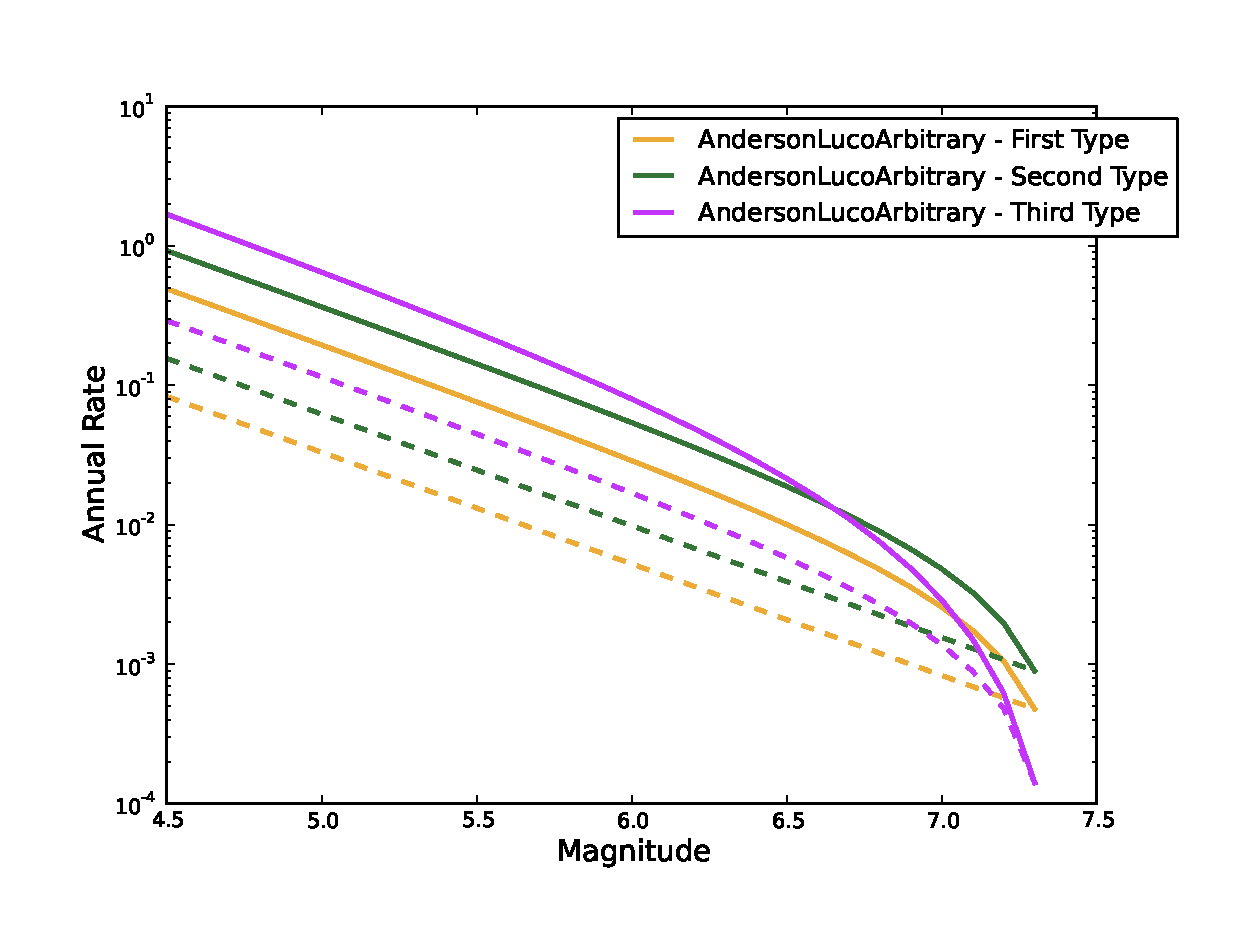
\includegraphics[trim=5mm 5mm 5mm 5mm, clip, width=12cm]{./figures/anderson_luco_arbitrary_mfds.eps}
  \caption{Comparison of magnitude frequency distributions for the specified fault using the three different models of the \cite{AndersonLuco1983} ``Arbitrary'' configuration}
  \label{fig:anderson_luco_arb}
\end{figure}
The models are then compared, as shown in Figure \ref{fig:anderson_luco_arb}, using the following commands:

\begin{Verbatim}[frame=single, commandchars=\\\{\}, fontsize=\scriptsize]
In [9]: anderson_luco_arb = [anderson_luco_config1,
                             anderson_luco_config2,
                             anderson_luco_config3]
\# Import geological recurrence model plotting function
In [10]: from hmtk.plotting.faults.geology_mfd_plot import plot_recurrence_models
In [11]: plot_recurrence_models(anderson_luco_arb,
                                area,
                                slip,
                                msr,
                                rake,
                                msr_sigma=0.0) \# Number of standard devations above
                                                # or below the median msr 
\end{Verbatim}



\subsubsection{\cite{AndersonLuco1983} ``Area Mmax''}

The second set of models from \cite{AndersonLuco1983} consider the case when the the recurrence model is referred to the rupture area of the maximum earthquake specified on the fault. As the area is not extracted directly from the geometry, additional information must be provided, namely the aspect ratio of ruptures on the fault and the displacement to length ratio ($\alpha$) of the fault \cite{Bungum2007}. This information is used to derived an additional parameter ($\beta$):

\begin{equation}
\beta=\sqrt{\frac{\alpha M_o \left( 0 \right)}{\mu W}}
\end{equation}

The three types of \cite{AndersonLuco1983} ``Area Mmax'' model are then calculated via:

\begin{enumerate}

\item Type 1 (``First'')

\begin{equation}
N \left( {M_W \geq M} \right) = \frac{\bar{d} - \bar{b}}{\bar{d}} \frac{\dot{s}}{\beta} \exp \left( {-\frac{\bar{d}}{2} M_{MAX}} \right) \exp \left( {\bar{b} \left[ {M_{MAX} - M} \right]} \right)
\end{equation}


\item Type 2 (``Second'')

\begin{equation}
N \left( {M_W \geq M} \right) = \frac{\bar{d} - \bar{b}}{\bar{b}}  \frac{\dot{s}}{\beta} \exp \left( {-\frac{\bar{d}}{2} M_{MAX}} \right)  \exp \left( {-\bar{b} \left[ {M_{MAX} - M} \right] - 1} \right)
\end{equation}

\item Type 3 (``Third'')

\begin{equation}
\begin{split}
N \left( {M_W \geq M} \right) = & \frac{\bar{d} \left( {\bar{d} - \bar{b}} \right)}{\bar{b}} \frac{\dot{s}}{\beta} \exp \left( {-\frac{\bar{d}}{2} M_{MAX}} \right) \times \ldots \\ 
& \left( {\frac{1}{\bar{b}} \left( {\exp \left( {\bar{b} \left[ {M_{MAX} - M} \right]} \right) - 1} \right) - \left[ {M_{MAX} - M} \right]} \right)
\end{split}
\end{equation}

\end{enumerate}

As the rupture aspect ratio and displacement to length ratio are attributes of the fault and not of the MFD, then the MFD configuration is the same as that of the \cite{AndersonLuco1983} ``Arbitrary'' calculator, albeit that \verb=Model_Name= must now be specified as \verb=AndersonLucoAreaMmax=. As before, the maximum magnitude and their uncertainty are optional, and will taken from the magnitude scaling relation if not specified in the configuration. This is permitted simply to ensure flexibility of the algorithm, although given the context of the ``Area MMax'' algorithm it is understood that the maximum magnitude should be interpreted by the modeller. If this is not the case, and the maximum magnitude is intended to be constrained using the geometry of the rupture, the ``Arbitrary'' model may be preferable.

\begin{figure}[htb]
  \centering
      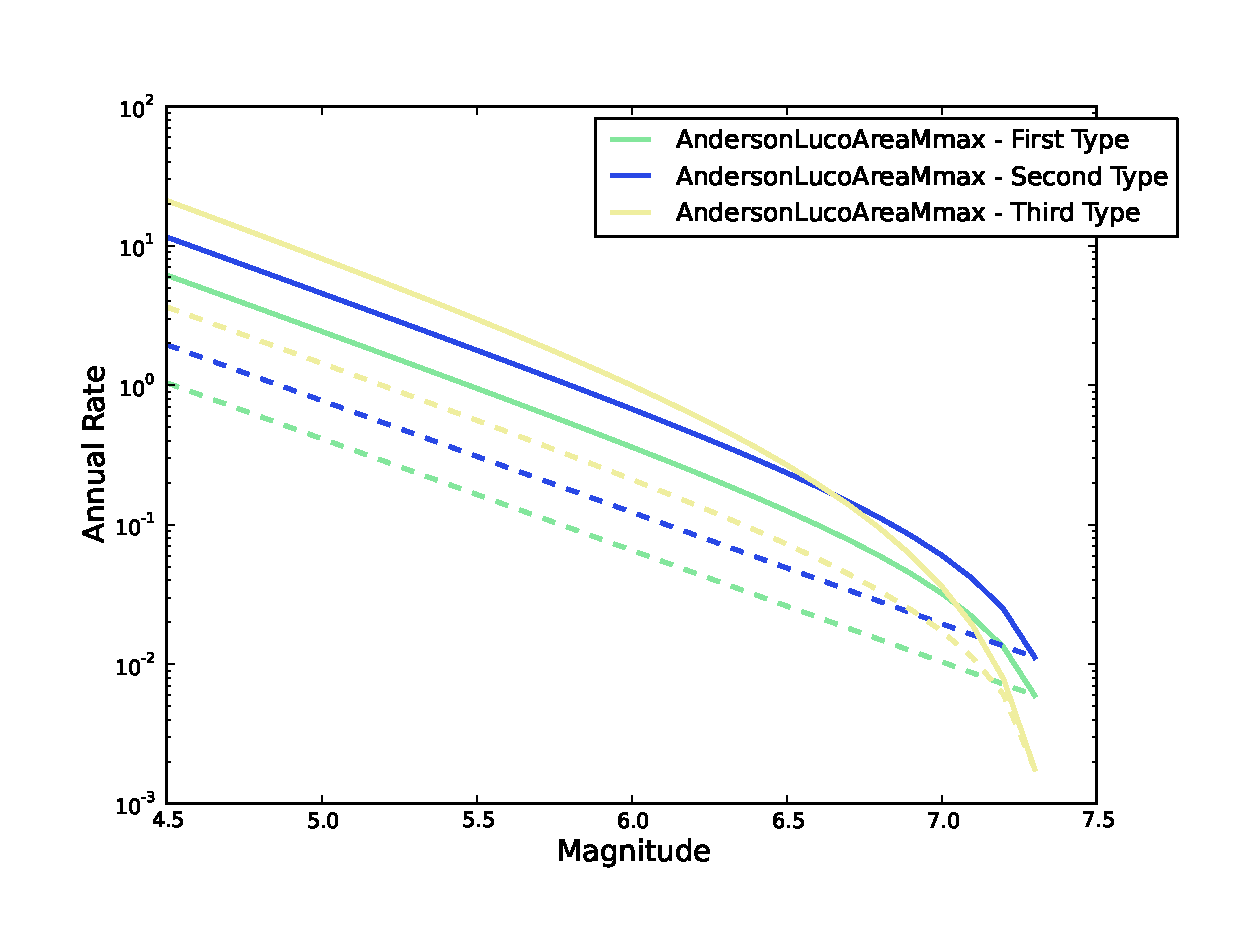
\includegraphics[trim=5mm 5mm 5mm 5mm, clip, width=12cm]{./figures/anderson_luco_mmax_mfds.eps}
  \caption{Comparison of magnitude frequency distributions for the specified fault using the three different models of the \cite{AndersonLuco1983} ``Area-Mmax'' configuration}
  \label{fig:anderson_luco_area_mmax}
\end{figure}

The three distributions can compared visually for the same fault using the plotting tools shown previously. The example below, using the same fault properties defined previously, will generate a plot similar to that shown in Figure \ref{fig:anderson_luco_area_mmax}.

\begin{Verbatim}[frame=single, commandchars=\\\{\}, fontsize=\scriptsize]
In [1]: anderson_luco_config1 = \{'Model_Name': 'AndersonLucoAreaMmax',
                                 'Model_Type': 'First',
                                 'Model_Weight': 1.0,  
                                 'MFD_spacing': 0.1,
                                 'Maximum_Magnitude': None,
                                 'Minimum_Magnitude': 4.5,
                                 'b_value': [0.8, 0.05]\}
In [2]: anderson_luco_config2 = \{'Model_Name': 'AndersonLucoAreaMmax',
                                 'Model_Type': 'Second',
                                 'Model_Weight': 1.0,
                                 'MFD_spacing': 0.1,
                                 'Maximum_Magnitude': None,
                                 'Minimum_Magnitude': 4.5,
                                 'b_value': [0.8, 0.05]\}
In [3]: anderson_luco_config3 = \{'Model_Name': 'AndersonLucoAreaMmax',
                                 'Model_Type': 'Third',
                                 'Model_Weight': 1.0,   
                                 'MFD_spacing': 0.1,
                                 'Maximum_Magnitude': None,
                                 'Minimum_Magnitude': 4.5,
                                 'b_value': [0.8, 0.05]\}
In [4]: anderson_luco_area_mmax = [anderson_luco_config1,
                                   anderson_luco_config2,
                                   anderson_luco_config3]
In [5]: plot_recurrence_models(anderson_luco_area_mmax,
                               area,
                               slip,
                               msr,
                               rake,
                               disp_length_ratio=1.25E-5, 
                               msr_sigma=0.0)

\end{Verbatim}

\subsubsection{Characteristic}

Although the term ``Characteristic'' may take on certain different meanings in the literature, in the present calculator it is referring to the circumstance when the fault is assumed to rupture with magnitudes distributed in a narrow range around the single characteristic magnitude. The model is therefore a truncated Gaussian distribution, in which the following must be specified: mean characteristic magnitude, the uncertainty (in magnitude units) and the number of standard deviations above and below the mean to be used as truncation limits.

\begin{Verbatim}[frame=single, commandchars=\\\{\}, fontsize=\scriptsize]
          \# Example of constructor for characteristic earthquake
        - Model_Type: Characteristic
          \# Spacing (magnitude units) of the magnitude frequency distribution
          MFD_spacing: 0.1
          \# Weight of the model
          Model_Weight: 0.2
          \# Magnitude of the Characteristic Earthquake
          Maximum_Magnitude:
          \# Uncertainty on Characteristic Magnitude (in magnitude units)
          Sigma: 0.12
          \# Lower bound truncation (in number of standard deviations)
          Lower_Bound: -3.0
          \# Upper bound truncation (in number of standard deviations)
          Upper_Bound: 3.0
\end{Verbatim}

The parameters \verb=Model_Type=, \verb= MFD_Spacing=, \verb=Model_Weight=, and\verb= Maximum_Magnitude= are as described for the previous calculators. \verb=Sigma= is the uncertainty of the characteristic magnitude (in magnitude units), and \verb=Lower_Bound= and \verb=Upper_Bound= are the lower and upper truncation limits of the Gaussian distribution respectively. Note that setting \verb=Sigma= to 0.0 or \verb=Lower_Bound= and \verb=Upper_Bound= to zero will simply result in the characteristic magnitude being evaluated as a single Dirac function.

\begin{figure}[htb]
  \centering
      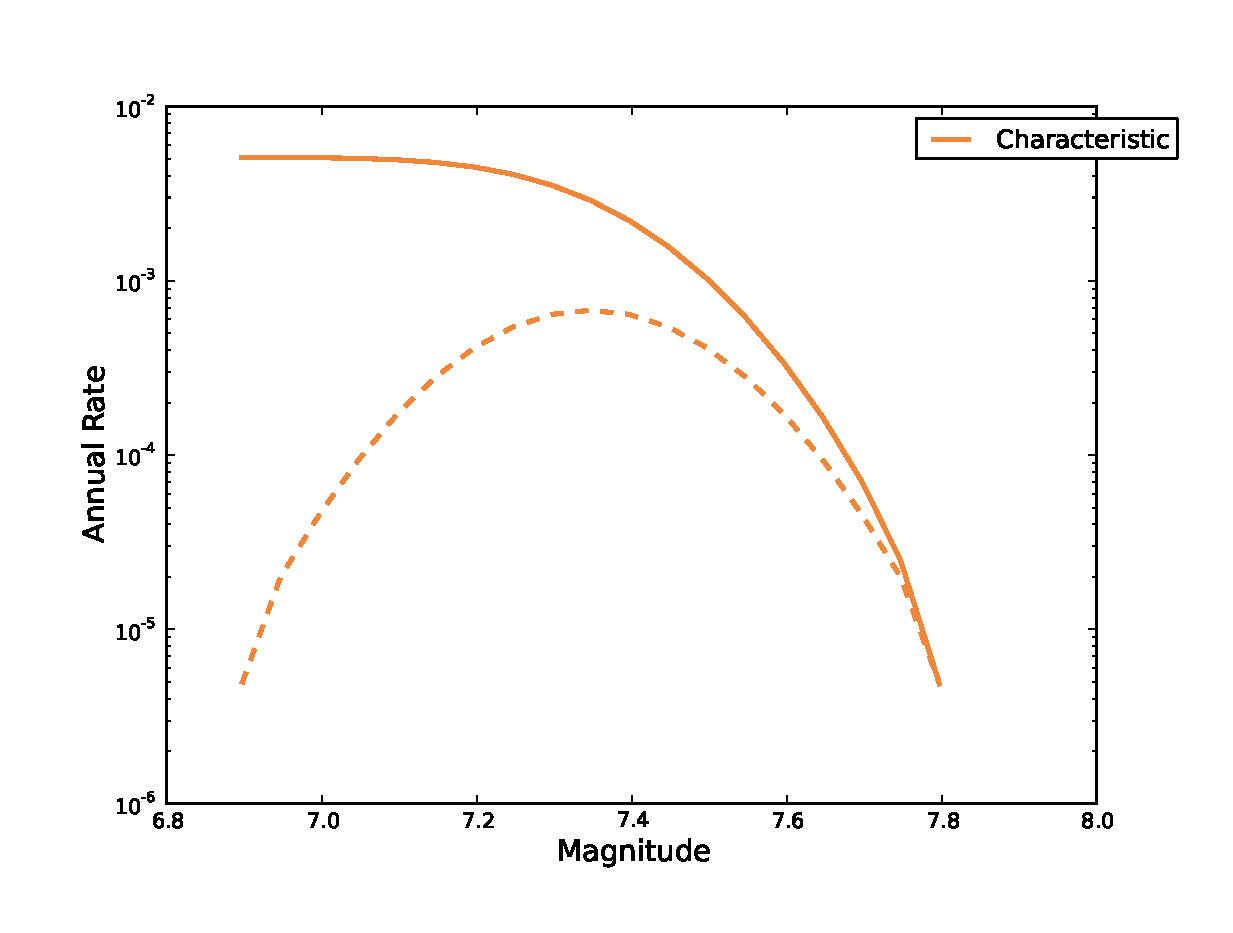
\includegraphics[trim=5mm 5mm 5mm 5mm, clip, width=12cm]{./figures/characteristic_mfds.eps}
  \caption{Magnitude frequency distribution for the specified fault configuration using the ``Characteristic'' model}
  \label{fig:characteristic}
\end{figure}

The distribution is shown, for the fault example defined previously, in Figure \ref{fig:characteristic}, which is generated using the code example shown below:

\begin{Verbatim}[frame=single, commandchars=\\\{\}, fontsize=\scriptsize]
In [1]: characteristic = [{'Model_Name': 'Characteristic',
                           'MFD_spacing': 0.05,
                           'Model_Weight': 1.0,
                           'Maximum_Magnitude': None,
                           'Sigma': 0.15, 
                           'Lower_Bound': -3.0, 
                           'Upper_Bound': 3.0}]
In [2]: plot_recurrence_models(characteristic,
                               area,
                               slip,
                               msr,
                               rake,
                               msr_sigma=0.0)
\end{Verbatim}                               



\subsubsection{\cite{YoungsCoppersmith1985} ``Exponential''}

This model is another form of ``Exponential'' model and is noted as being similar in construct to the \cite{AndersonLuco1983} Type 2 models. It is included here mostly for completeness. The model is given as:

\begin{equation}
N \left( {M_W \geq M} \right) = \frac{\mu A \dot{s} \left( {1.5 - b} \right) \left( {1 - \exp \left( {-\beta \left( {M_{MAX} - M} \right)} \right)} \right)}{b M_{0}^{MAX} \exp \left( {-\beta \left( {M_{MAX} - M} \right)} \right)}
\end{equation}
where $M_0^{MAX}$ is the moment corresponding to the maximum magnitude. The inputs for the model are defined in a similar manner as for the \cite{AndersonLuco1983} models:

\begin{Verbatim}[frame=single, commandchars=\\\{\}, fontsize=\scriptsize]
        - Model_Name: YoungsCoppersmithExponential
          \# Example constructor of the Youngs & Coppersmith (1985) Exponential model
          MFD_spacing: 0.1
          Model_Weight: 0.3
          Maximum_Magnitude:
          Maximum_Magnitude_Uncertainty:
          Minimum_Magnitude: 5.0
          b_value: [0.8, 0.05]
\end{Verbatim}

Note that all of the exponential models described here contain the term $d - b$, or some variant thereof, where $d$ is equal to 1.5. This introduces the condition that $b \leq 1.5$. 

\subsubsection{\cite{YoungsCoppersmith1985} ``Characteristic''}

The \cite{YoungsCoppersmith1985} model is a hybrid model, comprising an exponential distribution for lower magnitudes and a fixed recurrence rate for the characteristic magnitude $M_C$. The exponential component of the model is described via:

\begin{equation}
N \left( M \right) - N \left( {M_C} \right) = \frac{\mu A \dot{s}\ e^{\left( {-\beta \left( {M_{MAX} - M - 0.5} \right)}\right)} M_{0}^{MAX}}{1 - e^{\left( {-\beta \left( {M_{MAX} - M - 0.5} \right)} \right)}} 
 \left[ {\frac{b10^{-c/2}}{c - b} + \frac{b e^{\beta}\left({1 - 10^{-c/2}}\right)}{c}} \right]\end{equation}

where $\beta = b \ln \left( {10} \right)$, $c = 1.5$ and all other parameters are described as for the \cite{YoungsCoppersmith1985} ``Exponential'' and \cite{AndersonLuco1983} models. The rate for the characteristic magnitude is then given by:

\begin{equation}
N \left( {M_C} \right) = \frac{\beta \left( {N \left( M \right) - N \left( {M_C} \right)} \right) e^{-\beta \left( {M_{MAX} - M - 1.5} \right)}}{2 \left( {1 - e^{-\beta \left( {M_{MAX} - M - 1.5} \right)}} \right)}
\end{equation}

As described in \cite{YoungsCoppersmith1985}, this model assumes that:
\begin{enumerate}
\item The characteristic magnitude bin width $\Delta M_C$ is 0.5 $M_W$
\item Magnitudes are exponentially distributed up to a value $M'$, where $M' = M_{MAX} - \Delta M_C$
\item The absolute rate of characteristic earthquakes $\dot{M} \left( {M_C} \right)$ is approximately equal to $\dot{M} \left( {M' - 1} \right)$
\end{enumerate}

The current calculator adopts the implementation found in the \href{http://docs.openquake.org/oq-hazardlib/mfd.html#module-openquake.hazardlib.mfd.youngs_coppersmith_1985}{OpenQuake hazardlib}. At present, these three model assumptions are hard-coded, meaning that the distribution need only be defined from the moment rate and the characteristic magnitude. For [implementation] simplicity the input definition for the characteristic earthquake model is actually the same as for the exponential model. However, here the attribute \verb=Maximum_Magnitude= is actually referring to the characteristic magnitude and not to the absolute maximum magnitude, which will be 0.25 larger. 

\begin{figure}[htb]
  \centering
      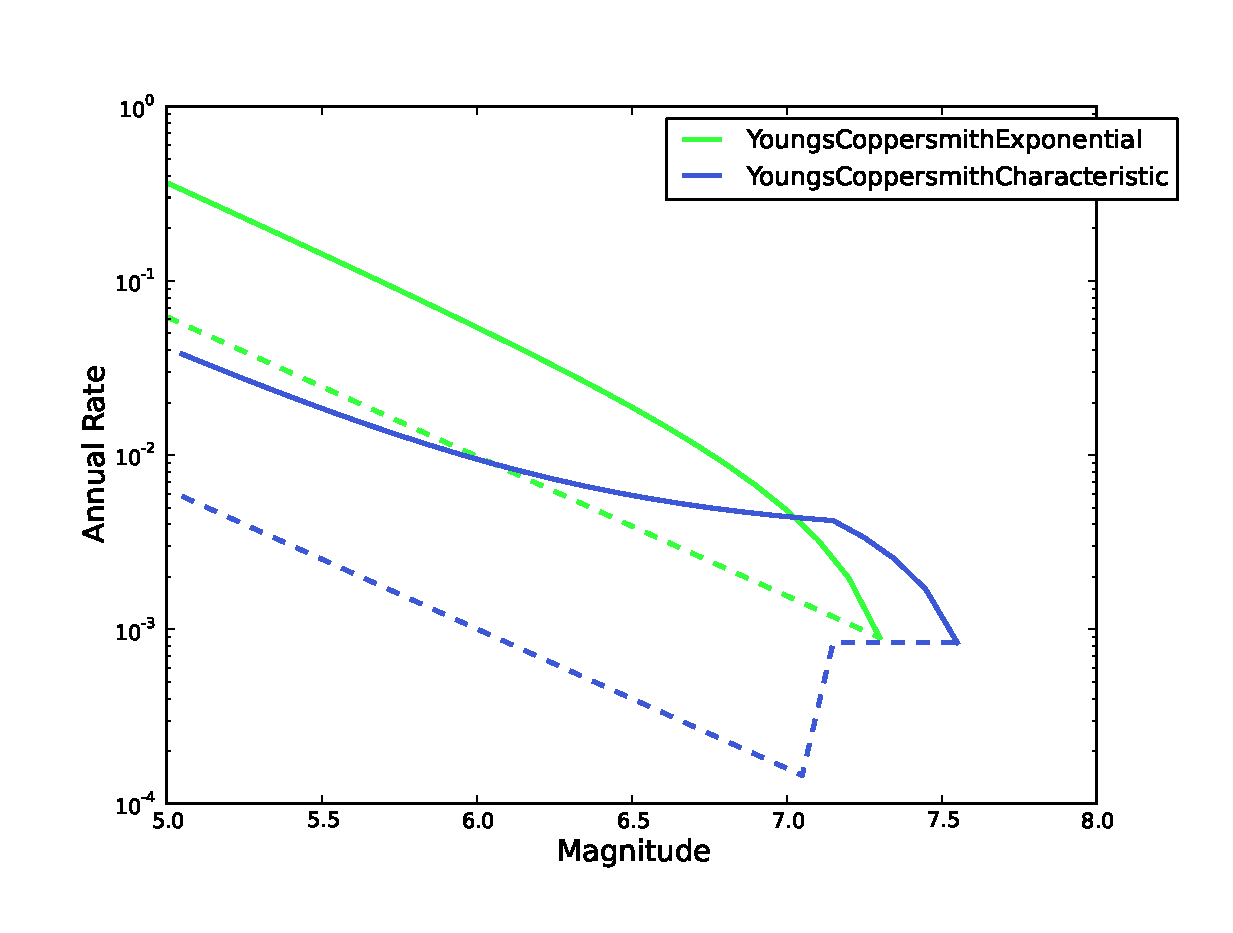
\includegraphics[trim=5mm 5mm 5mm 5mm, clip, width=12cm]{./figures/youngs_coppersmith_mfds.eps}
  \caption{Magnitude frequency distribution for the specified fault configuration using the \cite{YoungsCoppersmith1985} ``Exponential'' and ``Hybrid'' models}
  \label{fig:youngs_coppersmith}
\end{figure}

The two \cite{YoungsCoppersmith1985} distributions are compared in Figure \ref{fig:youngs_coppersmith}, which is generated using the code below:
\begin{Verbatim}[frame=single, commandchars=\\\{\}, fontsize=\scriptsize]
In [1]: exponential = \{'Model_Name': 'YoungsCoppersmithExponential',
                       'MFD_spacing': 0.1,
                       'Maximum_Magnitude': None,
                       'Maximum_Magnitude_Uncertainty': None,
                       'Minimum_Magnitude': 5.0,
                       'Model_Weight': 1.0,
                       'b_value': [0.8, 0.1]\}

In [2]: hybrid = \{'Model_Name': 'YoungsCoppersmithCharacteristic',
                  'MFD_spacing': 0.1,
                  'Maximum_Magnitude': None,
                  'Maximum_Magnitude_Uncertainty': None,
                  'Minimum_Magnitude': 5.0,
                  'Model_Weight': 1.0,
                  'b_value': [0.8, 0.1],
                  'delta_m': None\}

In [3]: youngs_coppersmith = [exponential, hybrid]

# View the corresponding magnitude recurrence model
In [4]: plot_recurrence_models(youngs_coppersmith,
                               area,
                               slip,
                               msr,
                               rake,
                               msr_sigma=0.0)
\end{Verbatim}

\subsection{Running a Recurrence Calculation from Geology}

The particulars of the geological workflow are largely established in the input definition, and not in the configuration file. Execution of the whole process is then relatively simple, so it is broken down here into two steps. The first step simply imports an appropriate parser and loads the fault source. The parser contains a method called \verb=read_file(x)= which takes as an input the desired mesh spacing (in km) used to create the mesh of the fault surface. In the example below this is set to 1.0 km, but for large complex faults (such as large subduction zones) it may be desirable to select a larger spacing to avoid storing a large mesh in RAM.

\begin{Verbatim}[frame=single, commandchars=\\\{\}, fontsize=\scriptsize]

In [1]: from hmtk.parsers.faults.fault_yaml_parser import FaultYmltoSource

In [2]: input_file = 'path/to/fault_model_file.yml'

In [3]: parser = FaultYmltoSource(input_file)

\# Spacing of the fault mesh (km) must be specified at input (here 1.0 km) 
In [4]: fault_model, tect_reg = parser.read_file(1.0)

\end{Verbatim}

In the second step, we simply execute the method to calculate the recurrence on the fault, and the write the resulting source model to an xml file. 

\begin{Verbatim}[frame=single, commandchars=\\\{\}, fontsize=\scriptsize]

\# Builds the fault model
In [5]: fault_model.build_fault_model()
\# Specify the xml file for writing the output model
In [6]: output_file  = 'path/to/output_source_model_file.yml'

In [7]: fault_model.source_model.serialise_to_nrml(outfile, use_defaults=True)
\end{Verbatim}

The serialiser takes as an optional input the choice to accept default values for certain attributes that may be missing from the fault source definition. These values are as follows:

\begin{table}[h]
\begin{tabular}{|c|c|} \hline
\textbf{Attribute} & \textbf{Default Value} \\ \hline
Aspect Ratio & 1.0 \\
Magnitude Scaling Relation & \cite{wells1994} ('WC1994') \\
Nodal Plane Distribution & Strike = 0., Dip = 90, Rake = 0., probability= 1.0\\
Hypocentral Depth Distribution & Depth = 10.0 km, Probability = 1.0 \\ \hline

\end{tabular}

\end{table}

\subsubsection{Epistemic Uncertainties}

The following example compares the case when epistemic uncertainties are incorporated into the analysis. A demonstration file (\verb=tests/parsers/faults/yaml_examples/=\\
\verb=simple_fault_example_4branch.yml=) is included, which considers two epistemic uncertainties for a specific fault: slip rate and magnitude frequency distribution type. The fault has two estimates of slip rate (5 $mm \ yr^{-1}$ and 7 $mm\ yr^{-1}$), each assigned a weighting of 0.5. Two magnitude frequency distribution types (Characteristic and \cite{AndersonLuco1983} ``Arbitrary'') are assigned, with weights of 0.7 and 0.3 respectively. The analysis is run, in the manner described previously. Firstly we consider the case when the different options are enumerated (the default option:

\begin{Verbatim}[frame=single, commandchars=\\\{\}, fontsize=\scriptsize]
In [1]: from hmtk.parsers.faults.fault_yaml_parser import FaultYmltoSource
In [2]: input_file = 'tests/parsers/faults/yaml_examples/simple_fault_example_4branch.yml'
In [3]: parser = FaultYmltoSource(input_file) 
In [4]: fault_model, tect_reg = parser.read_file(1.0)
In [5]: fault_model.build_fault_model()
In [6]: output_file  = 'path/to/output_source_model_file.yml'
In [7]: fault_model.source_model.serialise_to_nrml(output_file, use_defaults=True)
\end{Verbatim}

As four different activity rates are produced, the source is duplicated four time, each with an activity rate that corresponds to the rate calculated for the specific branch, multiplied by the weight of the branch. The output is a nrml file with four sources, as illustrated below:

\begin{Verbatim}[frame=single, commandchars=\\\{\}, fontsize=\scriptsize]
<?xml version='1.0' encoding='UTF-8'?>
<nrml xmlns:gml="http://www.opengis.net/gml" xmlns="http://openquake.org/xmlns/nrml/0.4">
  <sourceModel name="Template Simple Fault">
    <simpleFaultSource id="1_1" name="A Simple Fault" tectonicRegion="Active Shallow Crust">
      <simpleFaultGeometry>
        <gml:LineString>
          <gml:posList>30.0 30.0 30.0 31.0</gml:posList>
        </gml:LineString>
        <dip>30.0</dip>
        <upperSeismoDepth>0.0</upperSeismoDepth>
        <lowerSeismoDepth>20.0</lowerSeismoDepth>
      </simpleFaultGeometry>
      <magScaleRel>WC1994</magScaleRel>
      <ruptAspectRatio>1.5</ruptAspectRatio>
      <incrementalMFD minMag="6.64" binWidth="0.1">
        <occurRates>1.66984888376e-05 0.000165760464747 0.000658012622916 
                    0.00135343006814 0.00144508466725 0.00080109356265 
                    0.000230216031359 3.05523435745e-05 0.0</occurRates>
      </incrementalMFD>
      <rake>-90.0</rake>
    </simpleFaultSource>
    <simpleFaultSource id="1_2" name="A Simple Fault" tectonicRegion="Active Shallow Crust">
      <simpleFaultGeometry>
        <gml:LineString>
          <gml:posList>30.0 30.0 30.0 31.0</gml:posList>
        </gml:LineString>
        <dip>30.0</dip>
        <upperSeismoDepth>0.0</upperSeismoDepth>
        <lowerSeismoDepth>20.0</lowerSeismoDepth>
      </simpleFaultGeometry>
      <magScaleRel>WC1994</magScaleRel>
      <ruptAspectRatio>1.5</ruptAspectRatio>
      <incrementalMFD minMag="4.5" binWidth="0.1">
        <occurRates>0.0404671423911 0.033659102961 0.0279964224108 
                    0.0232864098818 0.0193687920987 0.0161102595577 
                    0.0133999302432 0.0111455765116 0.00927048675038
                    0.00771085501945 0.00641360984941 0.00533460831472
                    0.00443713392921 0.00369064724985 0.00306974667434
                    0.00255330407018 0.00212374582219 0.00176645483392
                    0.00146927313415 0.00122208816284 0.00101648865894
                    0.000845478440245 0.000703238335844 0.000584928170206
                    0.000486522060675 0.000404671423911</occurRates>
      </incrementalMFD>
      <rake>-90.0</rake>
    </simpleFaultSource>
    <simpleFaultSource id="1_3" name="A Simple Fault" tectonicRegion="Active Shallow Crust">
      <simpleFaultGeometry>
        <gml:LineString>
          <gml:posList>30.0 30.0 30.0 31.0</gml:posList>
        </gml:LineString>
        <dip>30.0</dip>
        <upperSeismoDepth>0.0</upperSeismoDepth>
        <lowerSeismoDepth>20.0</lowerSeismoDepth>
      </simpleFaultGeometry>
      <magScaleRel>WC1994</magScaleRel>
      <ruptAspectRatio>1.5</ruptAspectRatio>
      <incrementalMFD minMag="6.64" binWidth="0.1">
        <occurRates>2.33778843726e-05 0.000232064650645 0.000921217672083
                    0.0018948020954 0.00202311853414 0.00112153098771 
                    0.000322302443902 4.27732810043e-05 0.0</occurRates>
      </incrementalMFD>
      <rake>-90.0</rake>
    </simpleFaultSource>
    <simpleFaultSource id="1_4" name="A Simple Fault" tectonicRegion="Active Shallow Crust">
      <simpleFaultGeometry>
        <gml:LineString>
          <gml:posList>30.0 30.0 30.0 31.0</gml:posList>
        </gml:LineString>
        <dip>30.0</dip>
        <upperSeismoDepth>0.0</upperSeismoDepth>
        <lowerSeismoDepth>20.0</lowerSeismoDepth>
      </simpleFaultGeometry>
      <magScaleRel>WC1994</magScaleRel>
      <ruptAspectRatio>1.5</ruptAspectRatio>
      <incrementalMFD minMag="4.5" binWidth="0.1">
        <occurRates>0.0566539993476 0.0471227441454 0.0391949913751
                    0.0326009738345 0.0271163089382 0.0225543633808 
                    0.0187599023404 0.0156038071162 0.0129786814505
                    0.0107951970272 0.00897905378917 0.00746845164061
                    0.00621198750089 0.00516690614979 0.00429764534408
                    0.00357462569825 0.00297324415106 0.00247303676749
                    0.00205698238781 0.00171092342797 0.00142308412252
                    0.00118366981634 0.000984533670182 0.000818899438288
                    0.000681130884944 0.000566539993476</occurRates>
      </incrementalMFD>
      <rake>-90.0</rake>
    </simpleFaultSource>
  </sourceModel>
</nrml>
\end{Verbatim}

If, alternatively, the user wishes to collapse the logic tree branches to give a single source as an output, this option can be selected as follows:

\begin{Verbatim}[frame=single, commandchars=\\\{\}, fontsize=\scriptsize]
...
In [8]: from openquake.hazardlib.scalerel.wc1994 import WC1994
In [9]: fault_model.build_fault_model(collapse=True, rendered_msr=WC1994())
...
\end{Verbatim}

To collapse the branches it is simple necessary to specify as an input to the function \verb=collapse= \verb=True=. The second option requires further explanation. A seismogenic source requires the definition of a corresponding magnitude scaling relation, even if multiple scaling relations have been used as part of the epistemic uncertainty analysis. As collapsing the branches means that the activity rate is no longer associated with a specified scaling relation, but is an aggregate of many, the user must select the scaling relation to be associated with the output activity rate, for use in the OpenQuake hazard calculation. Therefore the input \verb=rendered_msr= must be given an instance of one of the supported magnitude scaling relationships.

The output file should resemble the following:

\begin{Verbatim}[frame=single, commandchars=\\\{\}, fontsize=\scriptsize]
<?xml version='1.0' encoding='UTF-8'?>
<nrml xmlns:gml="http://www.opengis.net/gml" xmlns="http://openquake.org/xmlns/nrml/0.4">
  <sourceModel name="Template Simple Fault">
    <simpleFaultSource id="1_1" name="A Simple Fault" tectonicRegion="Active Shallow Crust">
      <simpleFaultGeometry>
        <gml:LineString>
          <gml:posList>30.0 30.0 30.0 31.0</gml:posList>
        </gml:LineString>
        <dip>30.0</dip>
        <upperSeismoDepth>0.0</upperSeismoDepth>
        <lowerSeismoDepth>20.0</lowerSeismoDepth>
      </simpleFaultGeometry>
      <magScaleRel>WC1994</magScaleRel>
      <ruptAspectRatio>1.5</ruptAspectRatio>
      <incrementalMFD minMag="4.5" binWidth="0.1">
        <occurRates>0.0971211417387 0.0807818471064 0.0671914137858
                    0.0558873837162 0.0464851010369 0.0386646229385
                    0.0321598325836 0.0267493836278 0.0222491682009
                    0.0185060520467 0.0153926636386 0.0128030599553
                    0.0106491214301 0.00885755339963 0.00736739201842
                    0.00612792976843 0.00509698997324 0.00423949160142 
                    0.00352625552195 0.00293301159081 0.00243957278146
                    0.00202914825659 0.00184661595792 0.00231362389313
                    0.00360190992617 0.00434969292261 0.00243432469089
                    0.000909841780938 0.000164472079868 0.0</occurRates>
      </incrementalMFD>
      <rake>-90.0</rake>
    </simpleFaultSource>
  </sourceModel>
</nrml>
\end{Verbatim}


\cleardoublepage


% \cleardoublepage
% % -----------------------------------------------------------------------------
\chapter{Geodetic Tools}
\begin{myfancybox}
The objectives of this chapter are:
\begin{itemize}
    \item Describe features of the geodetic tools Hazard Modeller's Toolkit 
    \item Run simple calculations using the geodetic tools 
\end{itemize}
\end{myfancybox}
  \section{Recurrence from Geodetic Strain}

The final third workflow currently supported by the Hazard Modeller's toolkit is somewhat more experimental than the seismicity or geological workflows. The role that geodesy plays in directly constraining earthquake recurrence rates for active seismological structures and regions is becoming widely recognised. Whilst s standard methodology has not yet emerged, the tools constructed here are built around the ``Seismic Hazard Inferred from Tectonics (SHIFT)'' methodology originally proposed by \citet{BirdLiu2007} and applied on a global scale by \citet{Bird_etal2010}. The focus is placed on this model, in part, because it is fed by regional and/or global scale models of strain on a continuum. The initial global application, which underpins part of the present implementation, uses the first version of the Global Strain Rate Model \citep{Kreemer_etal2003}. The second version of the Global Strain Rate Model has been produced as part of the Global Earthquake Model, and it is anticipated that this will form a basis for many future uses of the present geodetic tools.

\subsection{The Recurrence Calculation}

The point of convergence between the geological and geodetic methodologies for estimating earthquake recurrence is in the definition of the total moment rate for an active seismogenic structure:
 \begin{equation}
 \dot{M}_o = c \mu A \dot{s}
 \end{equation}
 where A is the area of the coupled surface, $\dot{s}$ is the slip rate, $\mu$ the shear modulus and $c$ the coefficient describing the fraction of seismogenic coupling. Initially, the moment-rate tensor may be related to the strain rate tensor ($\epsilon_{ij}$) using the formula of \cite{Kostrov1974}:
 \begin{equation}
 \dot{M}_{oij} = 2 \mu H A \varepsilon_{ij}
 \end{equation}
 
 where H is the seismogenic thickness and A the area of the seismogenic source. Adopting the definition for a deforming continuum given by \citet{BirdLiu2007} the moment rate is equal to:
 
\begin{equation}
\dot{M}_o = A \left\langle {cz} \right\rangle \mu \left\{\begin{array}{lr}
2\dot{\varepsilon}_3 &:\dot{\varepsilon}_2 < 0\\
-2\dot{\varepsilon}_1&:\dot{\varepsilon}_2 \geq 0
\end{array}\right.
\end{equation}
 
 where assuming $\dot{\varepsilon}_1 \leq \dot{\varepsilon}_2 \leq \dot{\varepsilon}_3$ and $\dot{\varepsilon}_1 + \dot{\varepsilon}_2 + \dot{\varepsilon}_3 = 0$ (i.e. no volumetric changes are observed). The coupled seismogenic thickness ($\left\langle cz \right\rangle$) is a characteristic of each tectonic zone, and for the current purposes corresponds to the values (and regionalisation) proposed by \cite{BirdKagan2004}. 
 
 \subsubsection{The \cite{BirdLiu2007} Approach}
 
 As the regionalisation of \citet{BirdKagan2004} underpins the \cite{BirdLiu2007} methodology, the following approach is used to derive the shallow sesimicity rate. The geodetic moment rate  is first divided by the ``model'' moment rate ($\dot{M}_o^{CMT}$), which is the integral of the tapered Gutenberg-Richter distribution fit to the subset of the Global CMT catalogue for each tectonic zone, then multiplied by the number of events in the sub-catalogue ($N^{CMT}$) above the threshold (completeness) magnitude for the sub-catalogue ($m_T$):
 
 \begin{equation}
 \dot{N} \left( {m > m_T^{CMT}} \right) = \left( {\frac{\dot{M}_o}{\dot{M}_o^{CMT}}} \right) \dot{N}^{CMT}
 \end{equation}

The forecast rate of seismicity greater than $m_T$ ($\dot{N} \left( {m > m_T} \right)$) for a particular zone (or cell) is described using the tapered Gutenberg-Richter distribution:

\begin{equation}
\begin{split}
\dot{N} \left( {m > m_T} \right) =& \dot{N} \left( {m > m_T^{CMT}} \right) \left( {\frac{M_o \left( {m_T} \right)}{M_o \left( {m_T^{CMT}} \right)}} \right)^{-\beta} \times \ldots \\
& \exp \left( {\frac{M_o \left( {m_T^{CMT}} \right) - M_o \left( {m_T} \right)}{M_o \left( {m_c} \right)}} \right)\end{split}
\end{equation}
 
 
 \subsection{Running a Strain Calculation}
 \subsubsection{Strain File Format}
 
 As the current process considers only continuum models, a strain model can be input as a simple comma separated value (.csv) file. This is a basic text file with the following headers:
 
\begin{Verbatim}[frame=single, commandchars=\\\{\}, fontsize=\scriptsize]
longitude, latitude, exx, eyy, exy, region
45.0, -45., 0.0, 0.0, 0.0, IPL
.
.
.
177.0,-38.2,19.3,-37.0,-49.7,C
\end{Verbatim}

In the present format, the values \verb=exx, eyy, exy= describe the horizontal components of the strain tensor (in the example above in terms of nanostrain, $10^{-9}$). The \verb=region= term corresponds to the region (in this instance the \cite{Kreemer_etal2003} class) to which the cell belongs: Intra-plate [IPL], Subduction [S], Continental [C], Oceanic[O] and Ridge[R]. If the user does not have a previously defined regionalisation, can be determined using the $0.6^{\circ} \times 0.5^{\circ}$ global regionalisation cells.

The simplest strain workflow is to implement the model as defined by \cite{Bird_etal2010}. This process is illustrated in the following steps:

\begin{enumerate}

\item To simply load in the csv data the \verb=ReadStrainCsv= tool is used:

\begin{Verbatim}[frame=single, commandchars=\\\{\}, fontsize=\scriptsize]
In [1]: from hmtk.parsers.strain.strain_csv_parser import ReadStrainCsv, WriteStrainCsv

\# Load the file
In [2]: reader = ReadStrainCsv(''path/to/strain/file.csv'')

In [3]: strain_model = reader.read_data(scaling_factor=1E-9)

\end{Verbatim}

\item If the regionalisation is not supplied within the input file then it can be assigned initially from the in-built \cite{Kreemer_etal2003} regionalisation. This is done as follows (and may take time to execute depending on the size of the data):

\begin{Verbatim}[frame=single, commandchars=\\\{\}, fontsize=\scriptsize]
\# (Optional) To assign regionalisation from Kreemer et al. 2003
In [4]: from hmtk.strain.regionalisation.kreemer_regionalisation import  KreemerRegionalisation
\# (Optional)
In [5]: regionalisation = KreemerRegionalisation()
\# (Optional)
In [6]: strain_model = regionalisation.get_regionalisation(strain_model)
\end{Verbatim}

\item The next step is to implement the Shift calculations. The Shift module must first be imported and the magnitudes for which the activity rates are to be calculated must be defined as a list (or array). The strain data is input into the calculation along with two other configurable options: \verb=cumulative= decides whether it is the cumulative rate of events above each magnitude (\verb=True=), or the incremental activity rate for the bin $M \left( i \right):M \left( {i + 1} \right)$ (\verb=False=), \verb=in_seconds= decides whether to return the rates per second for consistency with \cite{Bird_etal2010} (\verb=True=) or as annual rates (\verb=False=). 

\begin{Verbatim}[frame=single, commandchars=\\\{\}, fontsize=\scriptsize]
In [7]: from hmtk.strain.shift import Shift

\# In this example, calculate cumulative rates for M > 5., 6., 7., 8.
In [8]: magnitudes = [5., 6., 7., 8.]

In [9]: model = Shift(magnitudes)

In [10]: model.calculate_activity_rate(strain_model, cumulative=False, in_seconds=False)

\end{Verbatim}

\item Finally the resulting model can be written to a csv file. This will be in the same format as the input file, now with additional attributes and activity rates calculated.

\begin{Verbatim}[frame=single, commandchars=\\\{\}, fontsize=\scriptsize]

\# Export the resulting rates to a csv file
In [11]: writer = WriteStrainCsv(''path/to/output/file.csv'')

In [12]: writer.write_file(model.strain, scaling_factor=1E-9)
\end{Verbatim}
\end{enumerate}


Additional support for writing a continuum model to a nrml Point Source model is envisaged, although further work is needed to determine the optimum approach for defining the seismogenic coupling depths, hypocentral depths and focal mechanisms. 
 



 
 
 
  



\cleardoublepage


% -----------------------------------------------------------------------------
\part{Appendices}
\appendix
% -----------------------------------------------------------------------------
% -----------------------------------------------------------------------------
\chapter{The 10 Minute Guide to Python!}
\label{sec:python_guide}
\begin{myfancybox}
 The objectives of this chapter are:
\begin{itemize}
     \item To introduce Python data types to facilitate use of the HMTK for Python beginners
 \end{itemize}
\end{myfancybox}
The HMTK is intended to be used by scientists and engineers without the necessity of having an existing knowledge of Python. It is hoped that the examples contained in this manual should provide enough context to allow the user to understand how to use the tools for their own needs. In spite of this, however, an understanding of the fundamentals of the Python programming language can greatly enhance the user experience and permit the user to join together the tools in a workflow that best matches their needs. 

The aim of this appendix is therefore to introduce some fundamentals of the Python programming language in order to help understand how, and why, the HMTK can be used in a specific manner. If the reader wishes to develop their knowledge of the Python programming language beyond the examples shown here, there is a considerable body of literature on the topic from both a scientific and developer perspective.

\section{Basic Data Types}

Fundamental to the use of the HMTK is an understanding of the basic data types Python recognises:


\subsection{Scalar Parameters}

\begin{itemize}
\item \textbf{float} A floating point (decimal) number. If the user wishes to enter in a floating point value then a decimal point must be included, even if the number is rounded to an integer.

\begin{python}[frame=single]
>> a = 3.5
>> print a, type(a)
3.5 <type 'float'>
\end{python}

\item \textbf{integer} An integer number. If the decimal point is omitted for a floating point number the number will be considered an integer

\begin{python}[frame=single]
>> b = 3
>> print b, type(b)
3 <type 'int'>
\end{python}

The functions \verb=float()= and \verb=int()= can convert an integer to a float and vice-versa. Note that taking \verb=int()= of a fraction will round the fraction down to the nearest integer

\begin{python}[frame=single]
>> float(b)
3
>> int(a)
3
\end{python}

\item \textbf{string} A text string (technically a ``list'' of text characters). The string is indicated by the quotation marks ''something'' or 'something else'

\begin{python}[frame=single]
>> c = "apples"
>> print c, type(c)
apples <type 'str'>
\end{python}

\item \textbf{bool} For logical operations python can recognise a variable with a boolean data type (\verb=True= / \verb=False=).

\begin{python}[frame=single]
>> d = True
>> if d:
       print "y"
   else:
       print "n"
y
>> d = False
>> if d:
       print "y"
   else:
       print "n"
n
\end{python}

\emph{Care should be taken in Python as the value 0 and 0.0 are both recognised as False if applied to a logical operation. Similarly, booleans can be used in arithmetic where True and False take the values 1 and 0 respectively}

\begin{python}[frame=single]
>> d = 1.0
>> if d:
       print "y"
   else:
       print "n"
y
>> d = 0.0
>> if d:
       print "y"
   else:
       print "n"
n
\end{python}
\end{itemize}

\subsubsection{Scalar Arithmetic}

Scalars support basic mathematical operations (\# indicates a comment):

\begin{python}[frame=single]
>> a = 3.0
>> b = 4.0
>> a + b # Addition
7.0
>> a * b # Multiplication
12.0
>> a - b # Subtraction
-1.0
>> a / b # Division
0.75
>> a ** b  # Exponentiation
81.0
# But integer behaviour can be different!
>> a = 3; b = 4
>> a / b
0
>> b / a
1
\end{python}

\subsection{Iterables}

Python can also define variables as lists, tuples and sets. These data types can form the basis for iterable operations. It should be noted that unlike other languages, such as Matlab or Fortran, Python iterable locations are zero-ordered (i.e. the first location in a list has an index value of 0, rather than 1). 

\begin{itemize}
\item \textbf{List} A simple list of objects, which have the same or different data types. Data in lists can be re-assigned or replaced
\begin{python}[frame=single]
>> a_list = [3.0, 4.0, 5.0]
>> print a_list
[3.0, 4.0, 5.0]
>> another_list = [3.0, "apples", False]
>> print another_list
[3.0, 'apples', False]
>> a_list[2] = -1.0
a_list = [3.0, 4.0, -1.0]
\end{python}

\item \textbf{Tuples} Collections of objects that can be iterated upon. As with lists, they can support mixed data types. However, objects in a tuple cannot be re-assigned or replaced.
\begin{python}[frame=single]
>> a_tuple = (3.0, "apples", False)
>> print a_tuple
(3.0, 'apples', False)
# Try re-assigning a value in a tuple
>> a_tuple[2] = -1.0
TypeError                Traceback (most recent call last)
<ipython-input-43-644687cfd23c> in <module>()
----> 1 a_tuple[2] = -1.0

TypeError: 'tuple' object does not support item assignment
\end{python}

\item \textbf{Range} A range is a convenient function to generate arithmetic progressions. They are called with a \verb=start=, a \verb=stop= and (optionally) a \verb=step= (which defaults to 1 if not specified)

\begin{python}[frame=single]
>> a = range(0, 5)
>> print a
[0, 1, 2, 3, 4]  # Note that the stop number is not 
                 # included in the set!  
>> b = range(0, 6, 2)
>> print b
[0, 2, 4]
\end{python}

\item \textbf{Sets} A set is a special case of an iterable in which the elements are unordered, but contains more enhanced mathematical set operations (such as intersection, union, difference, etc.)

\begin{python}[frame=single]
>> from sets import Set
>> x = Set([3.0, 4.0, 5.0, 8.0])
>> y = Set([4.0, 7.0])
>> x.union(y)
Set([3.0, 4.0, 5.0, 7.0, 8.0])
>> x.intersection(y)
Set([4.0])
>> x.difference(y)
Set([8.0, 3.0, 5.0]) # Notice the results are not ordered!
\end{python}
\end{itemize}

\subsubsection{Indexing}

For some iterables (including lists, sets and strings) Python allows for subsets of the iterable to be selected and returned as a new iterable. The selection of elements within the set is done according to the \verb=index= of the set. 

\begin{python}[frame=single]
>> x = range(0, 10)  # Create an iterable
>> print x
[0, 1, 2, 3, 4, 5, 6, 7, 8, 9]
>> print x[0] # Select the first element in the set
0             # recall that iterables are zero-ordered!
>> print x[-1] # Select the last element in the set
9
>> y = x[:] # Select all the elements in the set
>> print y
[0, 1, 2, 3, 4, 5, 6, 7, 8, 9]
>> y = x[:4]  # Select the first four element of the set
>> print y
[0, 1, 2, 3]
>> y = x[-3:] # Select the last three elements of the set
>> print y
[7, 8, 9]
>> y = x[4:7] # Select the 4th, 5th and 6th elements
>> print y
[4, 5, 6]
\end{python}

\subsection{Dictionaries}

Python is capable of storing multiple data types associated with a map of variable names inside a single object. This is called a ``Dictionary'', and works in a similar manner to a ``data structure'' in languages such as Matlab. Dictionaries are used frequently in the HMTK as ways of structuring inputs to functions that share a common behaviour but may take different numbers and types of parameters on input.

\begin{python}[frame=single]
>> earthquake = {"Name": "Parkfield",
                 "Year": 2004,
                 "Magnitude": 6.1,
                 "Recording Agencies" = ["USGS", "ISC"]}
# To call or view a particular element in a dictionary
>> print earthquake["Name"], earthquake["Magnitude"]
Parkfield 6.1
\end{python}

\subsection{Loops and Logicals}

Python's syntax for undertaking logical operations and iterable operations is relatively straightforward.

\subsubsection{Logical}

A simple logical branching structure can be defined as follows:

\begin{python}[frame=single]
>> a = 3.5
>> if a <= 1.0:
       b = a + 2.0
   elif a > 2.0:
       b = a - 1.0
   else:
       b = a ** 2.0
>> print b
2.5
\end{python}

Boolean operations can are simply rendered as \verb=and=, \verb=or= and \verb=not=.
\begin{python}[frame=single]
>> a = 3.5
>> if (a <= 1.0) or (a > 3.0):
       b = a - 1.0
   else:
       b = a ** 2.0
>> print b
2.5
\end{python}

\subsubsection{Looping}

There are several ways to apply looping in python. For simple mathematical operations, the simplest way is to make use of the \textbf{range} function:

\begin{python}[frame=single]
>> for i in range(0, 5):
       print i, i ** 2
0  0
1  1
2  4
3  9
4  16
\end{python}

The same could be achieved using the \verb=while= function (though possibly this approach is far less desirable depending on the circumstance):

\begin{python}[frame=single]
>> i = 0
>> while i < 5:
       print i, i ** 2
       i += 1
0  0
1  1
2  4
3  9
4  16
\end{python}

A \verb=for= loop can be applied to any iterable:

\begin{python}[frame=single]
>> fruit_data = ["apples", "oranges", "bananas", "lemons", 
                 "cherries"]
>> i = 0
>> for fruit in fruit_data:
       print i, fruit
       i += 1
0  apples
1  oranges
2  bananas
3  lemons
4  cherries 
\end{python}

The same results can be generated, arguably more cleanly, by making use of the \verb=enumerate= function:

\begin{python}[frame=single]
>> fruit_data = ["apples", "oranges", "bananas", "lemons", 
                 "cherries"]
>> for i, fruit in enumerate(fruit_data):
       print i, fruit
0  apples
1  oranges
2  bananas
3  lemons
4  cherries 
\end{python}

As with many other programming languages, Python contains the statements \verb=break= to break out of a loop, and \verb=continue= to pass to the next iteration.

\begin{python}[frame=single]
>> i = 0
>> while i < 10:
       if i == 3:
           i += 1
           continue
       elif i == 5:
           break
       else:
           print i, i ** 2
       i += 1
0  0
1  1
2  4
4  16
\end{python}

\section{Functions}

Python easily supports the definition of functions. A simple example is shown below. \emph{Pay careful attention to indentation and syntax!}

\begin{python}[frame=single]
>> def a_simple_multiplier(a, b):
       """
       Documentation string - tells the reader the function 
       will multiply two numbers, and return the result and
       the square of the result
       """
       c = a * b
       return c, c ** 2.0

>> x = a_simple_multiplier(3.0, 4.0)
>> print x
(12.0, 144.0)
\end{python}

In the above example the function returns two outputs. If only one output is assigned then that output will take the form of a tuple, where the elements correspond to each of the two outputs. To assign directly, simply do the following:

\begin{python}[frame=single]
>> x, y = a_simple_multiplier(3.0, 4.0)
>> print x
12.0
>> print y
144.0
\end{python}

\section{Classes and Inheritance}

Python is one of many languages that is fully object-oriented, and the use (and terminology) of objects is prevalent throughout the HMTK and this manual. A full treatise on the topic of object oriented programming in Python is beyond the scope of this manual and the reader is referred to one of the many textbooks on Python for more examples

\subsection{Simple Classes}

A class is an object that can hold both attributes and methods. For example, imagine we wish to convert an earthquake magnitude from one scale to another; however, if the earthquake occurred after a user-defined year we wish to use a different formula. This could be done by a method, but we can also use a class:

\begin{python}[frame=single]
>> class MagnitudeConverter(object):
       """
       Class to convert magnitudes from one scale to another
       """
       def __init__(self, converter_year):
           """
           """
           self.converter_year = converter_year
       
       def convert(self, magnitude, year):
           """
           Converts the magnitude from one scale to another
           """
           if year < self.converter_year:
               converted_magnitude = -0.3 + 1.2 * magnitude
           else:
               converted_magnitude = 0.1 + 0.94 * magnitude
           return converted_magnitude
                  
>> converter1 = MagnitudeConverter(1990)
>> mag_1 = converter1.convert(5.0, 1987)
>> print mag_1
5.7
>> mag_2 = converter1.convert(5.0, 1994)
>> print mag_2
4.8
# Now change the conversion year
>> converter2 = MagnitudeConverter(1995)
>> mag_1 = converter2.convert(5.0, 1987)
>> print mag_1
5.7
>> mag_2 = converter2.convert(5.0, 1994)
>> print mag_2
5.7  
\end{python}

In this example the class holds both the attribute \verb=converter_year= and the method to convert the magnitude. The class is created (or ``instantiated'') with only the information regarding the cut-off year to use the different conversion formulae. Then the class has a method to convert a specific magnitude depending on its year.

\subsection{Inheritance}

Classes can be useful in many ways in programming. One such way is due to the property of inheritance. This allows for classes to be created that can inherit the attributes and methods of another class, but permit the user to add on new attributes and/or modify methods. 

In the following example we create a new magnitude converter, which may work in the same way as the \verb=MagnitudeConverter= class, but with different conversion methods.

\begin{python}[frame=single]
>> class NewMagnitudeConverter(MagnitudeConverter):
       """
       A magnitude converter using different conversion
       formulae
       """
       def convert(self, magnitude, year):
           """
           Converts the magnitude from one scale to another
           - differently!!!
           """
           if year < self.converter_year:
               converted_magnitude = -0.1 + 1.05 * magnitude
           else:
               converted_magnitude = 0.4 + 0.8 * magnitude
           return converted_magnitude
# Now compare converters
>> converter1 = MagnitudeConverter(1990)
>> converter2 = NewMagnitudeConverter(1990)
>> mag1 = converter1.convert(5.0, 1987)
>> print mag1
5.7
>> mag2 = converter2.convert(5.0, 1987)
>> print mag2
5.15
>> mag3 = converter1.convert(5.0, 1994)
>> print mag3
4.8
>> mag4 = converter2.convert(5.0, 1994)
>> print mag4
4.4    
\end{python}

\subsection{Abstraction}

Inspection of the HMTK code (\href{https://github.com/gem/oq-engine}{https://github.com/gem/oq-engine} shows frequent usage of classes and inheritance. This is useful in our case if we wish to make available different methods for the same problem. In many cases the methods may have similar logic, or may provide the same types of outputs, but the specifics of the implementation may differ. Functions or attributes that are common to all methods can be placed in a ``Base Class'', permitting each implementation of a new method to inherit the ``Base Class'' and its functions/attributes/behaviour. The new method will simply modify those aspects of the base class that are required for the specific method in question. This allows functions to be used interchangeably, thus allowing for a "mapping" of data to specific methods. 

An example of abstraction is shown using our two magnitude converters shown previously. Imagine that a seismic recording network (named "XXX") has a model for converting from their locally recorded magnitude to a reference global scale (for the purposes of narrative, imagine that a change in recording procedures in 1990 results in a change of conversion model). A different recording network (named ``YYY'') has a different model for converting their local magnitude to a reference global scale (and we imagine they also changed their recording procedures, but they did so in 1994). We can create a mapping that would apply the correct conversion for each locally recorded magnitude in a short catalogue, provided we know the local magnitude, the year and the recording network.

\begin{python}[frame=single]
>> CONVERSION_MAP = {"XXX": MagnitudeConverter(1990),
                     "YYY": NewMagnitudeConverter(1994)}
>> earthquake_catalogue = [(5.0, "XXX", 1985),
                           (5.6, "YYY", 1992),
                           (4.8, "XXX", 1993),
                           (4.4, "YYY", 1997)]
>> for earthquake in earthquake_catalogue:
       converted_magnitude = \ # Line break for long lines!
           CONVERSION_MAP[earthquake[1]].convert(earthquake[0],
                                                 earthquake[2])
       print earthquake, converted_magnitude
(5.0, "XXX", 1985) 5.7
(5.6, "YYY", 1992) 5.78
(4.8, "XXX", 1993) 4.612
(4.4, "YYY", 1997) 3.92
\end{python}

So we have a simple magnitude homogenisor that applies the correct function depending on the network and year. It then becomes a very simple matter to add on new converters for new agencies; hence we have a ``toolkit'' of conversion functions!

\section{Numpy/Scipy}

Python has two powerful libraries for undertaking mathematical and scientific calculation, which are essential for the vast majority of scientific applications of Python: Numpy (for multi-dimensional array calculations) and Scipy (an extensive library of applications for maths, science and engineering). Both libraries are critical to both OpenQuake and the HMTK. Each package is so extensive that a comprehensive description requires a book in itself. Fortunately there is abundant documentation via the online help for Numpy \href{www.numpy.org}{www.numpy.org} and Scipy \href{www.scipy.org}{www.scipy.org}, so we do not need to go into detail here. 

The particular facet we focus upon is the way in which Numpy operates with respect to vector arithmatic. Users familiar with Matlab will recognise many similarities in the way the Numpy package undertakes array-based calculations. Likewise, as with Matlab, code that is well vectorised is signficantly faster and more efficient than the pure Python equivalent. 

The following shows how to undertake basic array arithmetic operations using the Numpy library

\begin{python}[frame=single]
>> import numpy as np
# Create two vectors of data, of equal length
>> x = np.array([3.0, 6.0, 12.0, 20.0])
>> y = np.array([1.0, 2.0, 3.0, 4.0])
# Basic arithmetic
>> x + y   # Addition (element-wise)
np.array([4.0, 8.0, 15.0, 24.0])
>> x + 2   # Addition of scalar
np.array([5.0, 8.0, 14.0, 22.0])
>> x * y   # Multiplication (element-wise)
np.array([3.0, 12.0, 36.0, 80.0])
>> x * 3.0   # Multiplication by scalar
np.array([9.0, 18.0, 36.0, 60.0])
>> x - y   # Subtraction (element-wise)
np.array([2.0, 4.0, 9.0, 16.0])
>> x - 1.0   # Subtraction of scalar
np.array([2.0, 5.0, 11.0, 19.0])
>> x / y   # Division (element-wise)
np.array([3.0, 3.0, 4.0, 5.0])
>> x / 2.0   # Division over scalar
np.array([1.5, 3.0, 6.0, 10.0])
>> x ** y    # Exponentiation (element-wise)
np.array([3.0, 36.0, 1728.0, 160000.0])
>> x ** 2.0   # Exponentiation (by scalar)
np.array([9.0, 36.0, 144.0, 400.0])
\end{python}

Numpy contains a vast set of mathematical functions that can be operated on a vector (e.g.):

\begin{python}[frame=single]
>> x = np.array([3.0, 6.0, 12.0, 20.0])
>> np.exp(x)
np.array([2.00855369e+01, 4.03428793e+02, 1.62754791e+05,
         4.85165195e+08])
# Trigonometry
>> theta = np.array([0., np.pi / 2.0, np.pi, 1.5 * np.pi])
>> np.sin(theta)
np.array([0.0000, 1.0000, 0.0000, -1.0000])
>> np.cos(theta)
np.array([1.0000, 0.0000, -1.0000, 0.0000])
\end{python}

Some of the most powerful functions of Numpy, however, come from its logical indexing:

\begin{python}[frame=single]
>> x = np.array([3.0, 5.0, 12.0, 21.0, 43.0])
>> idx = x >= 10.0   # Perform a logical operation
>> print idx
np.array([False, False, True, True, True])
>> x[idx]   # Return an array consisting of elements
            # for which the logical operation returned True
np.array([12.0, 21.0, 43.0])
\end{python}

Create, index and slice n-dimensional arrays:

\begin{python}[frame=single]
>> x = np.array([[3.0,  5.0, 12.0, 21.0, 43.0],
                 [2.0,  1.0,  4.0, 12.0, 30.0],
                 [1.0, -4.0, -2.1,  0.0, 92.0]])
>> np.shape(x)
(3, 5)
>> x[:, 0]
np.array([3.0, 2.0, 1.0])
>> x[1, :]
np.array([2.0, 1.0, 4.0, 12.0, 30.0])
>> x[:, [1, 4]]
np.array([[ 5.0, 43.0],
          [ 1.0, 30.0],
          [-4.0, 92.0]])
\end{python}

The reader is referred to the online documentation for the full set of functions!



% -----------------------------------------------------------------------------
% -----------------------------------------------------------------------------
%\cleardoublepage
\bibliographystyle{apalike}
\bibliography{./bibliography/hazard}
\cleardoublepage
\printglossaries
\printindex
% -----------------------------------------------------------------------------
% -----------------------------------------------------------------------------
\end{document}
